\documentclass{article}

% NeurIPS 2025 formatting
%\usepackage{neurips_2025}
\usepackage[preprint]{neurips_2025} % Ensure this is the desired option (preprint, final, etc.)
% \usepackage{neurips_2025} 
\usepackage{natbib}
\bibliographystyle{plainnat} % Moved from end of doc to preamble for consistency

% Additional packages
\usepackage[utf8]{inputenc} % allow utf-8 input
\usepackage[T1]{fontenc}    % use 8-bit T1 fonts
\usepackage{hyperref}       % hyperlinks
\hypersetup{
    colorlinks=false,  % Don't color the links
    % pdfborder={0 0 0}, % No border around links (set to 0)
    % hidelinks         % Hide all visual cues of links
}
\usepackage{url}            % simple URL typesetting
\usepackage{booktabs}       % professional-quality tables
\usepackage{amsfonts}       % blackboard math symbols
\usepackage{nicefrac}       % compact symbols for 1/2, etc.
\usepackage{microtype}      % microtypography
\usepackage[usenames,dvipsnames]{xcolor}         % colors
\usepackage{amsmath,amssymb,amsthm}
\usepackage{enumitem}
\usepackage{geometry} % Consider adjusting margins if needed, or removing if default is fine
\usepackage{tikz}
\usepackage{graphicx}
\usetikzlibrary{arrows.meta,positioning,fit,backgrounds,calc}
\graphicspath{{./POC/figures/}{./paper/images/}{./figures/}} % Added POC and figures to graphicspath

%%%% Macros
\newcommand{\Loss}{\mathcal{L}}
\newcommand{\R}{\mathbb{R}}
\newcommand{\E}{\mathbb{E}}
\newcommand{\He}{\mathrm{He}}

% Macros for convenience
\newcommand{\BaseW}{\widetilde{w}}
\newcommand{\BaseG}{\widetilde{G}}
\newcommand{\BaseV}{\widetilde{V}}
\newcommand{\BaseE}{\widetilde{E}}

\newcommand{\ManifoldD}{\mathcal{M}_{D}}
\newcommand{\ManifoldRE}{\mathcal{M}_{RE}}
\newcommand{\ManifoldCE}{\mathcal{M}_{CE}}
\newcommand{\ManifoldBC}{\mathcal{M}_{BC}}
\newcommand{\LinSpaceLBC}{L_{BC}} % Linear space of block-constant matrices

% Comments:
% \newcommand{\giulia}[1]{{\color{ForestGreen}\textbf{Giulia:} #1}} % Keep for author's internal review if needed
%\newcommand{\giulia}[1]{} % Uncomment to hide comments

\usepackage[textsize=tiny]{todonotes}
% \usepackage{colortbl}

\newcommand{\mf}[1]{\todo[color=orange!30,size=\tiny]{MF: #1}}
\newcommand{\keivan}[1]{\todo[color=blue!30,size=\tiny]{K1: #1}}
\newcommand{\ff}[1]{\todo[color=blue!30,size=\tiny]{FF: #1}}
\newcommand{\AJ}[1]{\todo[color=green!30,size=\tiny]{AJ: #1}}
\newcommand{\GIU}[1]{\todo[color=purple!30,size=\tiny]{GIU: #1}}
\newcommand{\IMZ}[1]{\todo[color=red!30,size=\tiny]{IMAN: #1}}
%%%% Theorem environments
\newtheorem{definition}{Definition}[section]
\newtheorem{lemma}{Lemma}[section]
\newtheorem{proposition}{Proposition}[section]
\newtheorem{corollary}{Corollary}[section]
\newtheorem{remark}{Remark}[section]
\newtheorem{observation}{Observation}[section] % Added observation environment
\newtheorem{example}{Example}[section] % Added example environment
\numberwithin{figure}{section}


\title{Barriers for Learning in an Evolving World: \\a Mathematical Understanding of Loss of Plasticity}

\author{%
  Amir Joudaki$^{1}$ \And
  Giulia Lanzillotta$^{1}$ \And
  Mohammad Samragh Razlighi$^{2}$ \And
  Iman Mirzadeh$^{2}$ \And
  Keivan Alizadeh$^{2}$ \And
  Thomas Hofmann$^{1}$ \And
  Mehrdad Farajtabar$^{2}$ \And
  Fartash Faghri$^{2}$ %\And
  %\vspace{-20pt}
  \\
  $^{1}$ETH Zürich \quad
  $^{2}$Apple \\
  \texttt{amir.joudaki@inf.ethz.ch},
  \texttt{\{fartash, m\_farajtabar\}@apple.com}
  %\texttt{\{amir.joudaki, giulia.lanzillotta, thomas.hofmann\}@inf.ethz.ch} \\
  %\texttt{\{fartash, m\_samraghrazlighi, imirzadeh, kalizadehvahid, m\_farajtabar\}@apple.com}
}

\begin{document}
\maketitle

\begin{abstract}
    Standard deep learning models excel when trained on stationary datasets but often falter in non-stationary environments where continuous adaptation is crucial. This paradigm struggle is significantly due to the degradation of future learning capacity, a phenomenon termed loss of plasticity (LoP). This work undertakes a first-principles investigation into the mechanisms underlying LoP in gradient-based models. We propose a formal definition of LoP grounded in dynamical systems theory, identifying stable manifolds in the parameter space that act as traps for gradient trajectories. Our analysis details two specific mechanisms leading to such traps: frozen units arising from activation saturation and cloned-unit manifolds resulting from representational redundancy. Furthermore, we explore conditions under which architectural choices or targeted perturbations might prevent or mitigate this plasticity collapse.
    A core finding of our theoretical framework is the revelation of a fundamental tension: properties widely considered beneficial for generalization in conventional, static learning regimes, often characterized by distinct training and deployment phases, such as the emergence of low-rank representations or inherent simplicity biases, appear to directly contribute to LoP in continual learning scenarios.
    % \GIU{I think this last part of the abstract is a bit vague and redundant, I would remove it.}By mathematically characterizing these barriers, this work pinpoints critical representational properties that hinder continuous learning, providing a clear direction for developing truly adaptive artificial intelligence.
    Our theoretical analysis is supported by numerical simulations and empirical observations on various neural network architectures.
\end{abstract}

\section{Introduction}
% (Content from original draft - appears generally fine, ensure it leads into the new structure)
The extraordinary success of back-propagation in training deep neural networks often relies on two implicit, yet critical, assumptions. First, \emph{stationarity}: the data distribution encountered during training is assumed to be identical, or very similar, to the distribution faced during deployment, rendering post-training adaptation minimal or absent. Second, \emph{single random initialization}: diversity and exploration potential are primarily introduced through a single random initialization of network parameters, a resource that is progressively consumed by optimization and not replenished. These assumptions falter when an artificial agent must operate and learn continuously within an environment characterized by changing dynamics or evolving task distributions. This scenario, often termed continual or lifelong learning, presents a significant challenge known as the stability-plasticity dilemma \citep{abraham2005memory, chaudhry2018riemannian}: the system must be stable enough to retain previously acquired knowledge, yet plastic enough to integrate new information effectively.

Empirically, standard deep networks subjected to long sequences of tasks or slowly drifting data streams often exhibit a decline in their learning capability \citep{dohare2024loss, berariu2021plasticity, dohare2021continual, nikishin2022primacy, lyle2023understanding}. This phenomenon, termed loss of plasticity (LoP), is distinct from catastrophic forgetting \citep{mccloskey1989catastrophic, ratcliff1990connectionist, french1999catastrophic}, where new learning overwrites old knowledge. LoP specifically refers to the diminished ability to learn new information effectively over time. Common symptoms include exploding weight magnitudes \citep{nikishin2022primacy}, activation saturation, the emergence of ``dead'' ReLU units (whose upstream parameters cease to update) \citep{nair2010rectified, sokar2023dormant, dohare2021continual, lyle2022understanding}, a collapse in the effective rank of hidden layer representations indicating reduced feature diversity \citep{papyan2020prevalence, huh2022lowrank, kumar2020implicit, gulcehre2022empirical}, and redundancy or diminishing contributions from network components like attention heads or filters \citep{lyle2023understanding}. Many of these issues have been highlighted in recent studies focusing on LoP \citep{dohare2023maintaining, kumar2024regenerative, ash2020warmstarting}.

\citet{dohare2024loss} argue compellingly that such failures are intrinsically linked to the back-propagation algorithm itself. They posit that gradient descent, optimized for transient, single-task learning, relies heavily on the initial random state for exploration, a resource that is consumed and not replenished during prolonged training. Their work demonstrates that standard deep learning methods can lose plasticity until they perform comparably to linear networks, and suggests that maintaining plasticity requires mechanisms beyond pure gradient descent, such as continually injecting diversity via methods like their proposed continual backpropagation.

\paragraph{Goal of this paper.}
Motivated by observations about LoP, our paper revisits the dynamics of gradient descent and back-propagation through the lens of dynamical systems theory. We seek to answer the fundamental question:
\begin{quote}
\emph{What structural features inherent in gradient flow dynamics inevitably lead to LoP, and how might we design algorithms or architectures capable of perpetual adaptation?}
\end{quote}
The central proposition advanced in this work is that the tendency of gradient-based optimization to favor low-rank or ``simple'' representations lies at the heart of plasticity loss. While properties like low effective rank and simplicity bias are often associated with improved generalization in the standard two-phase learning paradigm \citep{huh2022lowrank, papyan2020prevalence, zhang2017understanding}, we argue that these very properties become detrimental in continual learning settings. By reducing the effective dimensionality of the network's feature space, they limit its capacity to adapt to novel information, thus contributing to the LoP observed by \citep{dohare2024loss} and others. Our work aims to provide a formal mathematical understanding of these mechanisms.
% \GIU{okay general comments on the new structure: I like it, the sections feel less chaotic, they are more homogeneous and complete The link between the section and an overview of the paper contributions is missing. Although I usually like the papers that take their time to tell you a story, I think it would help the reader to understand how the story is spread out. In particular I would say in the introduction something like "First, in section 3 we show how typical symptoms of LoP can emerge naturally during training with GD" and "Subsequently, in Section 4, we prove how the emergence of this attributes leads the network to permanently lose plasticity" You could even change the tone of the introduction entirely and be more "aggressive" in a sense, with a clear list of contributions like "we prove this ... we show that..." in bullet points. But I personally like the softer open question style that we have now}

To systematically address this, our investigation unfolds as follows.
In Section~\ref{sec:preliminaries}, we establish the necessary mathematical preliminaries, including our dynamical systems-based definition of LoP.
Section~\ref{sec:emergence_lop} then delves into how characteristics commonly associated with LoP, such as frozen units and representational redundancies, can naturally emerge from the interplay of linear transformations and non-linear activations during standard gradient-based training.
Building on this, Section~\ref{sec:existence_lop_manifold} formalizes the concept of LoP manifolds, proving that these emergent features can indeed trap gradient descent dynamics, thereby leading to a persistent loss of plasticity.
We then explore practical implications in Section~\ref{sec:mitigation_recovery}, discussing strategies to prevent the formation of these LoP states or to recover plasticity once they have manifested.
Finally, Section~\ref{sec:discussion} summarizes our findings, highlights the fundamental tension between generalization in static settings and adaptability in dynamic ones, and outlines promising avenues for future research towards truly continual learning systems.
% \GIU{Nice!!}


\section{Preliminaries}
\label{sec:preliminaries}
In this section, we lay the groundwork for our analysis by defining Loss of Plasticity (LoP) within a dynamical systems framework and recalling the standard definitions for feed-forward neural networks and back-propagation. The stability of LoP manifolds, a crucial concept for understanding their persistence, will be discussed later in Section~\ref{sec:existence_lop_manifold}.

Let $\theta\in\Theta\subseteq\R^p$ represent the parameters of a neural network. We consider training on a stream of data $\{(x_i,y_i)\}_{i=1}^N$ using gradient descent or its stochastic variants. The objective is typically to minimize a loss $\sum_{i=1}^N \Loss(\hat{y}_\theta(x_i),y_i),$ which we can succinctly refer to as $\Loss(\theta)$. The learning dynamics can be idealized by the continuous-time gradient flow:
\begin{equation}
    \frac{d\theta(t)}{dt} \;=\; -\nabla_\theta\Loss\bigl(\theta(t)\bigr).
    \label{eq:grad_flow}
\end{equation}
This perspective allows us to analyze the trajectory of parameters $\theta(t)$ in the parameter space $\Theta$ as driven by the negative gradient in the loss landscape.

\begin{definition}[LoP Manifold]
\label{def:lop}
A manifold $\mathcal{M}\subset\Theta$ induces LoP if the gradient of the loss function is tangent to the manifold at every point on the manifold. That is, $\nabla_\theta\Loss(\theta)\in T_\theta\mathcal{M}$ for all $\theta\in\mathcal{M}$, where $T_\theta\mathcal{M}$ denotes the tangent space of $\mathcal{M}$ at $\theta$. This tangency condition ensures that once the gradient flow enters $\mathcal{M}$, it remains within $\mathcal{M}$ under the dynamics of Equation~\ref{eq:grad_flow}.
\end{definition}


\begin{remark}
If the conditions in Definition~\ref{def:lop} hold irrespective of the specific data distribution generating the loss $\Loss$, which we can think of as functional LoP, and is our primary area of interest. Such LoP arises from the network architecture and gradient descent dynamics alone and is particularly relevant as it persists even if the task or data distribution evolves.
\end{remark}



\section{Emergence of LoP Symptoms: A First-Principles Perspective}
\label{sec:emergence_lop}
\label{sec:emergence_lop_first_principles}

The capacity of a neural network to continually learn is fundamentally tied to its ability to maintain a diverse and adaptable set of internal representations. However, as reported extensively in LoP literature, prolonged training or sequential task learning often leads to two critical detrimental phenomena: the emergence of frozen or dead units that cease to update their parameters, and a diminishing diversity of representations, where features become redundant or collapse into a lower-dimensional space \citep{dohare2021continual, lyle2022understanding, nikishin2022primacy}. In this section, we adopt a first-principles approach to understand why these LoP-inducing features might naturally arise as a consequence of the learning dynamics in deep neural networks.

At a high level, effective feature learning in a deep neural network involves a delicate balance. On one hand, the network must learn a rich set of features to expand its expressive power and accurately model complex data. On the other hand, for robust generalization, there is often an implicit or explicit bias towards simpler representations \citep{valle2018deep, zhang2017understanding}. The drive towards simplification in later training stages, where within-class feature variability collapses and class means adopt specific geometric configurations, is well-documented as \emph{neural collapse}~\citep{papyan2020prevalence}. We propose that the inherent tension between these two opposing forces---the need to create rich, diverse features that nonetheless remain ``simple'' enough to generalize---can naturally lead to the emergence of frozen units and representational redundancies, the hallmarks of LoP.

To make our notion of representational richness or diversity more precise, we will quantify it through the rank of the feature activations. 
One of the main ways of measuring diversity of a set of representations is the notion of \emph{hard rank}, or simply rank of a matrix, defined as the number of linearly independent rows or columns, which equals the number of its non-zero singular values. 
This is in contrast to \emph{effective rank}~\citep{dohare2024loss}, which provides a continuous measure of rank based on the distribution of singular values, defined as $\exp(H)$ where $H$ denotes the entropy of normalized singular values $H = -\sum_k p_i \log p_i, \; p_i = e_i/\sum_k e_i.$ 
% However, as the hard rank is often too stringent for practical purposes, we use the notion of effective rank~\citep{dohare2024loss}, defined as $\exp(H$ where $H$ denotes the entropy of normalized singular values $H = \sum_k p_i \log p_i, \; p_i = e_i/\sum_k e_i.$ 

% \GIU{I think this last part does not say anything much? I would remove it and go directly to the meat.} As empirically observed (see Appendix~\ref{app:empirical_evidence_appendix} and Figures~\ref{fig:emergence_lop_symptoms_cl}, \ref{fig:dupfrac-LoP}, \ref{fig:dupfrac-LoP-dead-dup}), and supported by theoretical analyses, this rank is dynamically shaped by the interplay of linear transformations and non-linear activations. This back-and-forth aims to learn rich features while being guided by the simplifying bias inherent in parts of the network.


\paragraph{Linear Layers and Rank Reduction}
Linear layers in neural networks, which are essentially matrix multiplications (followed by a bias), inherently tend to reduce or constrain the dimensionality of representations. Let us recount several important facts about matrix products which underscore their inability to unilaterally increase rank. First, the rank of a product of matrices cannot exceed the minimum rank of any matrix in the product, i.e., $\mathrm{rank}(AB) \le \min(\mathrm{rank}(A), \mathrm{rank}(B))$. Thus, a chain of linear operations can, at best, maintain rank but often reduces it. Second, the condition number of a product of matrices can worsen compared to individual matrices, potentially making features less distinguishable and thereby reducing the effective rank. Finally,  For deep linear networks or long chains of matrix products, particularly with random matrices, there's a strong tendency for the representation to collapse towards low-rank structures, sometimes even rank-one \citep{saxe2014exact, furstenberg1963noncommuting}.
This inherent rank-reducing nature of linear transformations means that non-linearities are crucial for creating and maintaining feature diversity.

\paragraph{Non-linear Activations and Rank Recovery.}
Non-linear activation functions are the primary mechanism by which neural networks can counteract the rank-reducing effects of linear layers and expand the dimensionality of learned representations. Informally, even if input features are highly correlated (implying low effective rank), a sufficiently non-linear activation can transform them in such a way that they become more distinct, increasing both the absolute number of independent features (hard rank) and their effective diversity.   
To make this more formal, consider a matrix of pre-activations $X \in \R^{n \times d}$ ($n$ samples, $d$ features with $n\ge d$), where each row is independently drawn from a multivariate Gaussian distribution $\mathcal{N}(0, C)$, with $C$ being the covariance matrix (unit diagonals, off-diagonals strictly in $(-1,1)$). Let $f: \R \to \R$ be an element-wise non-linear activation function.

\begin{proposition}[Rank recovery with non-linear activations]
\label{prop:rank_recovery_informal}
\label{prop:hard_rank_increase_main} %Changed label to avoid conflict
Let us assume that  $f$ is not a bounded degree polynomial, and that $\E f(z)^2,$ where $z\sim N(0,1)$ is bounded, and define post-activation covariance $C_f = \frac1n \E f(X)^\top f(X).$ First, $C_f$ has full rank, even if the input features $X$ is rank-deficient. Second, if the input features are highly correlated with effective rank $1+\epsilon$ for some small constant $\epsilon>0,$ effective rank of $C_f$ will be approximately  $1 + \alpha_f \epsilon,$ with the coefficient defined as $\alpha_f = \frac{\E f'(z)^2}{\E f(z)^2 } - 1$ with $z\sim N(0,1).$
\end{proposition}
The formal statement and proof details, based on Hermite polynomial expansions of $f$, are provided in Appendix~\ref{app:theory_appendix}. In light of this theory, we can think of $\alpha$ as a rank improvement strength of an activation.

\begin{remark}
\label{rem:duplicate_rank}
    The proposition above reveals an important insight that, both in hard rank and effective rank case, as long as pre-activation correlations are within $(-1,1),$ their post-activations will be hard rank and improved effective rank. Thus, one way of countering this will be to create duplicate features, where the activation will be unable to decouple.
    %  
\end{remark}

This theory reveals an important insight that non-linear activations indeed recover both hard rank and effective rank.  One natural question is, what can we say if the pre-activations deviate from standard Gaussian, e.g., if the pre-activations are distributed as $x\sim N(\mu,\sigma^2).$ This question is particularly relevant considering that training dynamics can dramatically shift distribution of pre-activations. It turns out that we can view this distributional shift as a way of modulating the activation. For example, in case of non-standard Gaussian pre-activation, we can control its mean and standard deviation into the activation, by shaping the activation $f(\mu + \sigma z)$ where $z\sim N(0,1)$. Thus, we view  changes in pre-activation statistics as a transformation the activation function itself. The following example sheds more light on this notion.

\begin{example}
For $f(x) = \tanh(ax)$. If $a$ is small, $\tanh(ax) \approx ax$, behaving linearly, with $\alpha$ converging to $0.$ On the other hand, if $a$ is very large, $\tanh(ax)$ approaches a sign function, and $\alpha$ tends to infinity.   
For $f(x) = \text{ReLU}(a x + b)$. If $b $ is a large positive shift, $f(x)$ will be mostly an affine transform $f(x) = a x + b, $ which cannot recover rank, but for non-positive shifts $b \le 0, $ it will maintain its non-linearity. 
% You can see an illustration of this in Figure~\ref{fig:theory_tanh_az_rank}.
\end{example}

\begin{figure}[ht!]
    \centering
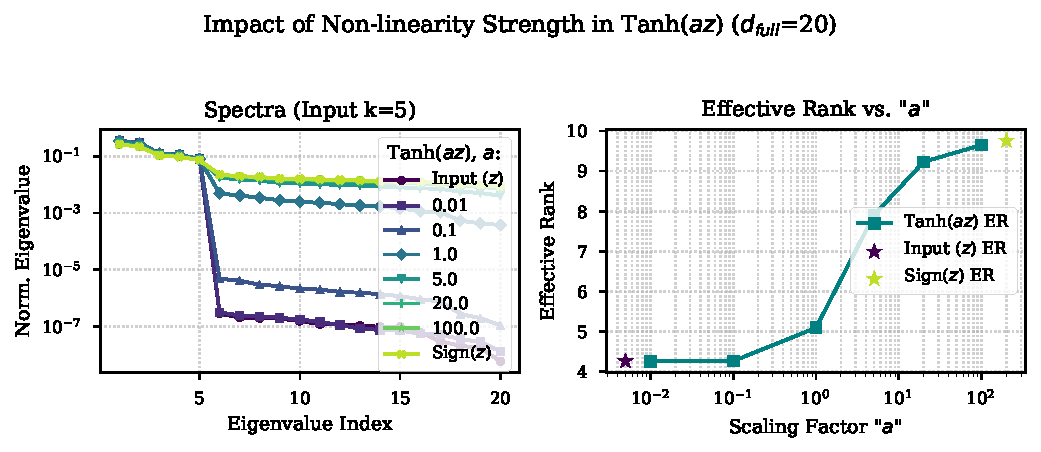
\includegraphics[width=0.7\linewidth]{POC/figures/theory_tanh_az_rank.pdf} % Assuming image is in figures/
    \vspace{-.3cm}
    \caption{Effect of input shifting on post-activation effective rank for $h_a = \tanh(a x)$, with rank-deficient $z$ ($20$ dimensional with rank $5$). \emph{Left:} Normalized eigenvalue spectra of $\mathrm{Cov}(h)$ vs. scale $a.$ \emph{Right:} Effective rank of $\mathrm{Cov}(h)$ vs. scale $a$. }
    \label{fig:theory_tanh_az_rank}
\end{figure}


This modulation has a critical consequence, revealed by the following corollary.

\begin{corollary}
\label{cor:max_alpha_frozen_formal}
Suppose an activation function $f_s$ is parameterized by $s \in S$, where $S$ is a parameter space (e.g., $S = \mathbb{R}$ for scaling, $S = \mathbb{R}^2$ for scale-shift). Assume that for all $s \in S$, $f_s$ has a finite Gaussian kernel, i.e., $\E[f_s(z)^2] < \infty$ for $z \sim \mathcal{N}(0,1)$.
If there exists a sequence of parameters $(s_k)_{k=1}^\infty \subset S$ such that: (i) The rank recovery strength $\alpha_{f_{s_k}} \to \infty$ as $k \to \infty$.
(ii) The expected squared value remains uniformly bounded, i.e., there is a constant $M < \infty$ such that $\E[f_{s_k}(z)^2] \le M$ for all $k$.
Then, the derivative $f'_{s_k}(z)$ tends to zero in probability as $k \to \infty$. That is, for any $\epsilon > 0$:
$$ \lim_{k \to \infty} P(|f'_{s_k}(z)| < \epsilon) = 1, \quad \text{for } z \sim \mathcal{N}(0,1). $$
\end{corollary}

The above corollary is stating that if we continuously adjust an activation function, e.g., by shifting or scaling its pre-activations, to maximize its rank recovery strength ($\alpha$), this process often drives the activation into a regime where its derivative is zero for almost all inputs, hence becoming ``frozen'' and stop learning. You can see Appendix~\ref{app:max_rank_frozen} for a proof of this corollary. We can get a better intuitive understanding of this statement by going back to the example of Tanh.\AJ{Consider FF's point about a potential connection to lazy training here. This phenomenon might resemble lazy training regimes under certain scaling limits, especially with full-rank random initializations. Would a brief mention or discussion be appropriate?}

\begin{example}
For $f(x) = \tanh(ax)$, the larger values of $a$ will lead to larger values of $\alpha_f.$ However, observe that in the limit of $\lim_{a \to \infty} \tanh(a x) = \text{sign}(x),$ we have $f'=0$ almost everywhere except $x=0.$ 
% In the case of ReLU $f(x) = \text{relu}(ax + b),$ we can tend $\alpha_f$ to by choosing $a,b$ such that $b/a \to -\infty,$ would also imply that $f' = 0 $ with probability $1$ when $z\sim N(0,1).$
\end{example}

% \GIU{This conclusion needs to be expanded on.} 
% (Giulia's trys) 
Taken together, Proposition \ref{prop:hard_rank_increase_main} and Corollary \ref{cor:max_alpha_frozen_formal}, tell us that activation functions are a double-edged sword when it comes to feature rank. On one hand, when the modulation is present, the non-linearity allows rank recovery for low-rank pre-activations, while on the other hand, if the modulation strength  is too high, the activation function can lead to frozen units.    
The key message of the corollary and the example above is  that frozen features may emerge as a natural tendency towards finding rich and diverse features while learning. 
% \GIU{Where did the ReLU example go?}

\paragraph{The Emergence of LoP Symptoms from Optimization Dynamics.} The symptoms of LoP---frozen units and diminished representational diversity (via rank collapse or feature duplication)---can be seen as natural outcomes of the network's learning dynamics. By learning to modulate pre-activation statistics and feature correlations, the network navigates the trade-off between generating rich, high-dimensional features necessary for complex tasks and simplifying representations, perhaps to improve generalization or to settle into stable attractors in the loss landscape.  However, moving too far in any direction may lead the network to Loss of Plasticity: aggressively increasing rank via strong non-linearity risks creating frozen units, i.e., Corollary~\ref{cor:max_alpha_frozen_formal}, while simplifying representations can lead to rank collapse or creation of duplicate features, i.e., Remark~\ref{rem:duplicate_rank}.

\subsection{Experimental Setup}
%  
To validate our theoretical insights, we conducted experiments across four architectures (MLP, CNN, ResNet, ViT) on continual learning tasks using Tiny ImageNet dataset, which consists of $200$ classes. Each architecture was trained on a sequence of $40$ tasks, with each task containing a disjoint subset of $5$ classes. We tracked the emergence of LoP symptoms including dead units (neurons with near-zero activations), duplicate units (highly correlated neurons with correlation > 0.95), and effective rank degradation. All experiments used Adam optimizer with learning rate 0.001 (0.0001 for ViT), and results are averaged over 5 random seeds. Training proceeds sequentially through the 40 tasks. Figures showing training progression over 'steps' reflect this continuous process; refer to Appendix~\ref{app:empirical_evidence_appendix} for specifics on steps per task and task switching protocol. Full experimental details are provided in Appendix~\ref{app:empirical_evidence_appendix}.
\AJ{Excellent point, there was a small inconsistency here before which is now fixed (we have 40 tasks not 10), and each task is trained for 500 epochs, so the 25000 steps corresponds to this plus the validation steps. Is it important to fix the plots or just explain it in text? }


The experimental evidence confirms these intuitions (see Appendix~\ref{app:empirical_evidence_appendix} and Figures~\ref{fig:emergence_lop_symptoms_cl}, \ref{fig:norm-rank-nG}, \ref{fig:dupfrac-LoP}, \ref{fig:dupfrac-LoP-dead-dup}): depending on the architecture, we observe that a degradation in the model performance is concomitant with the emergence of duplicate or frozen units, and a corresponding decrese in representational diversity. 

\begin{figure}[!h]
    \centering
    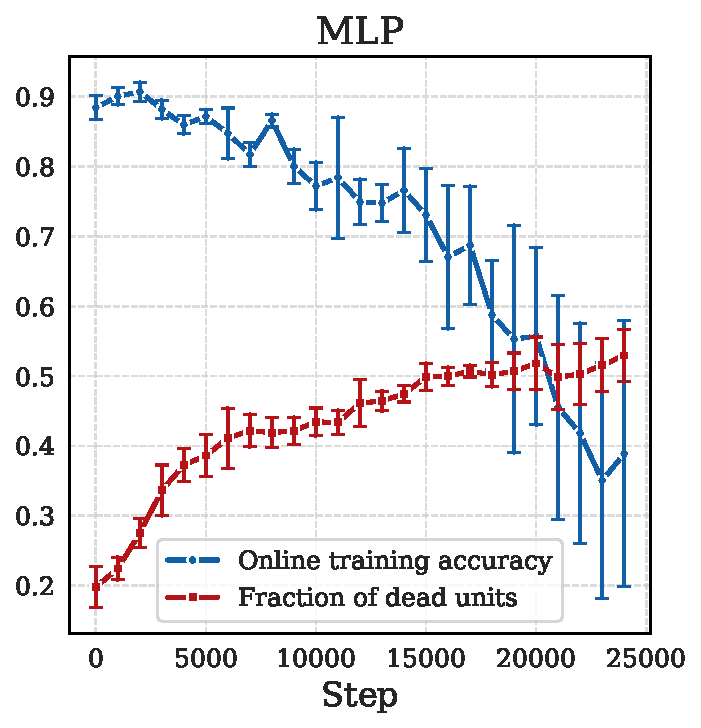
\includegraphics[width=0.23\linewidth]{paper/images/mlp_act__dead_fraction_plot.pdf}
    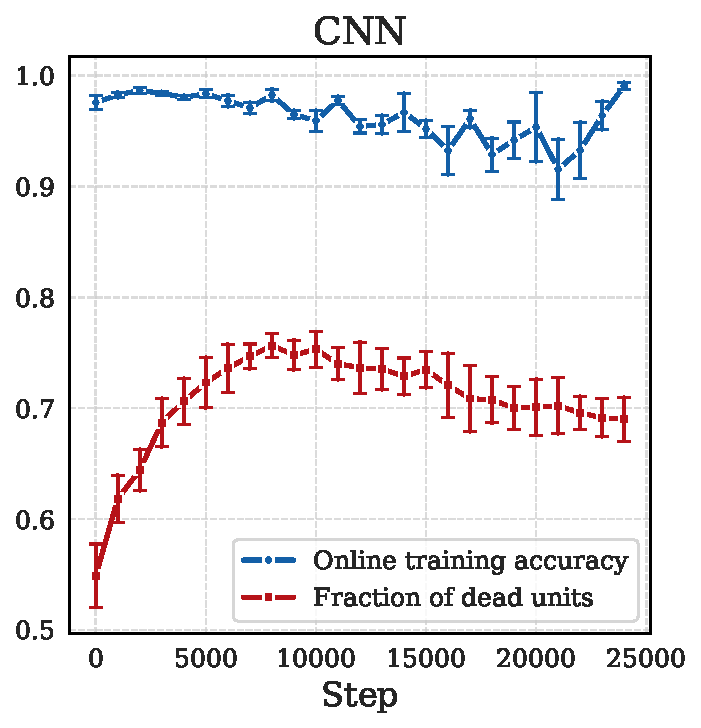
\includegraphics[width=0.23\linewidth]{paper/images/cnn_act__dead_fraction_plot.pdf}
    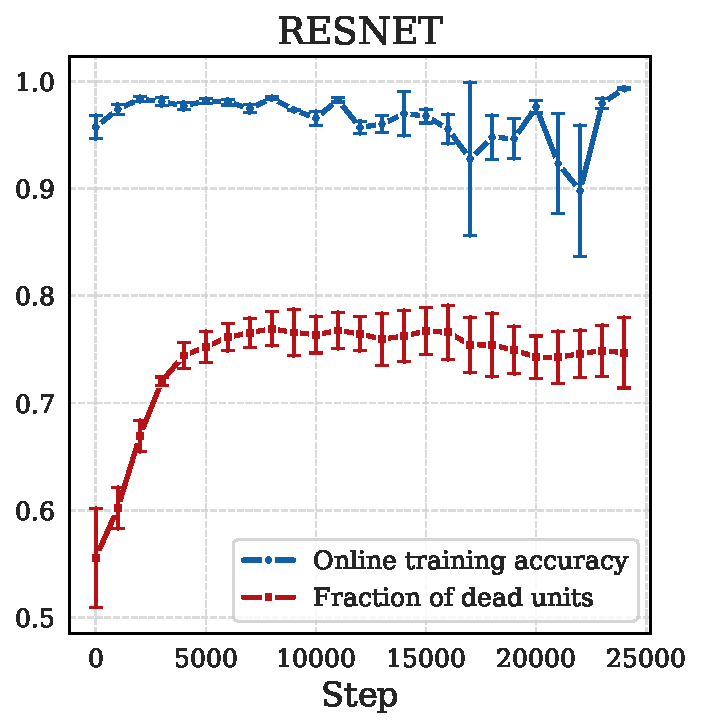
\includegraphics[width=0.23\linewidth]{paper/images/resnet_block_dead_fraction_plot.pdf}
    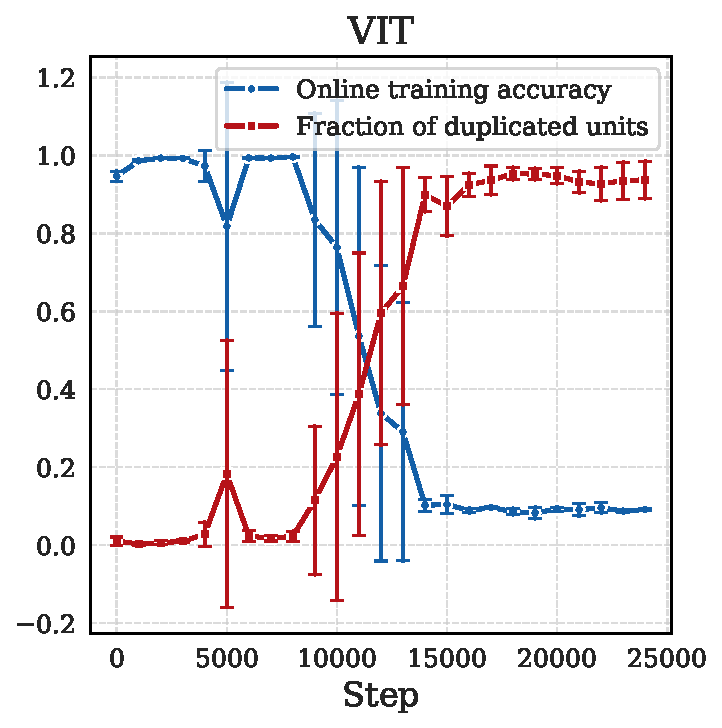
\includegraphics[width=0.24\linewidth]{paper/images/vit_block_dup_fraction_plot.pdf}
        \vspace{-.3cm}
    \caption{Causes and symptoms of Loss of Plasticity emerging during continual learning. The plots illustrate (across different architectures like MLP, CNN, ResNet, and ViT from left to right) an increase in the fraction of dead or duplicate units during training, coincidental with a decrease in training accuracy. These are key indicators of LoP. The 'Training Accuracy' refers to an evolving measure of performance across tasks (specific definition in Appendix~\ref{app:empirical_evidence_appendix}, cf. Figure~\ref{fig:normalizations-recovering} caption). (Details of experimental setup in Appendix~\ref{app:empirical_evidence_appendix}).}
    \label{fig:emergence_lop_symptoms_cl}
\end{figure}

\begin{figure}[!h]
    \centering
    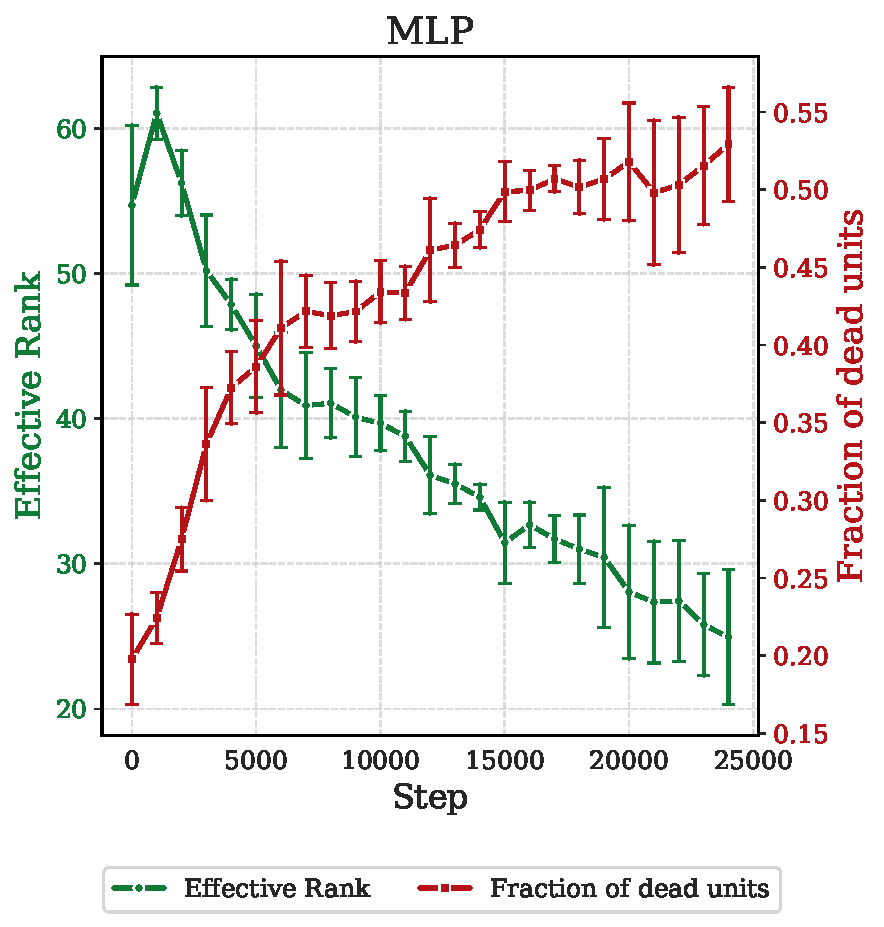
\includegraphics[width=0.24\linewidth]{paper/images/mlp_act__rankdead_plot.pdf}
    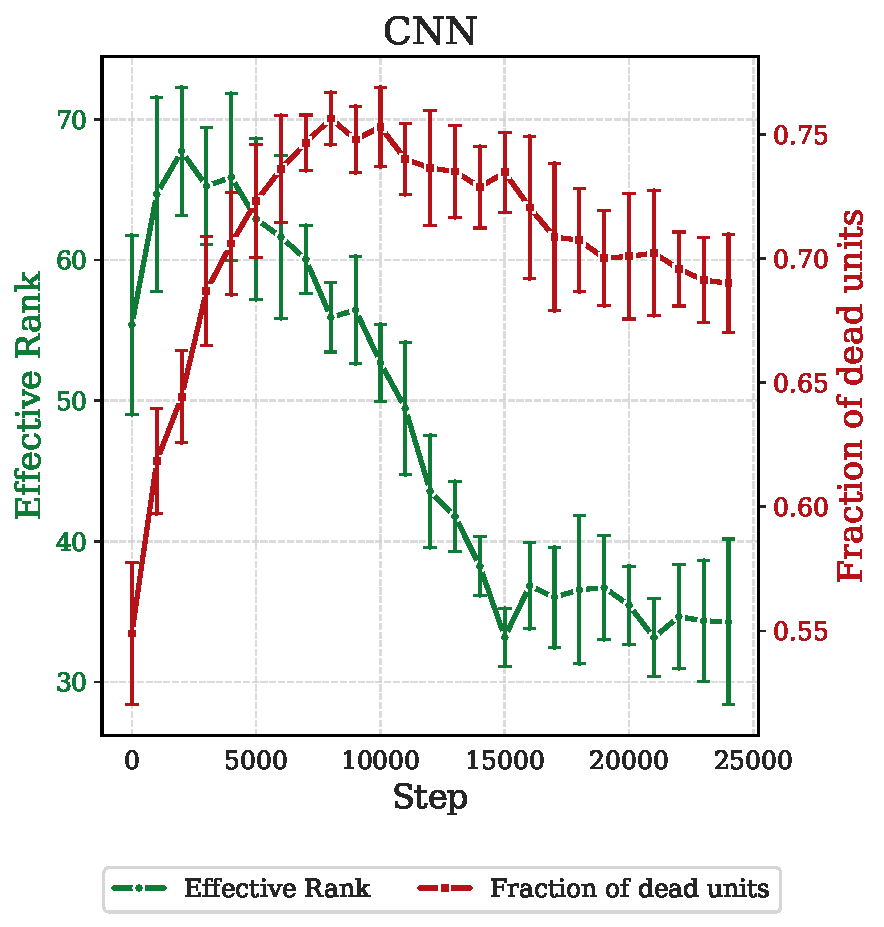
\includegraphics[width=0.24\linewidth]{paper/images/cnn_act__rankdead_plot.pdf}
    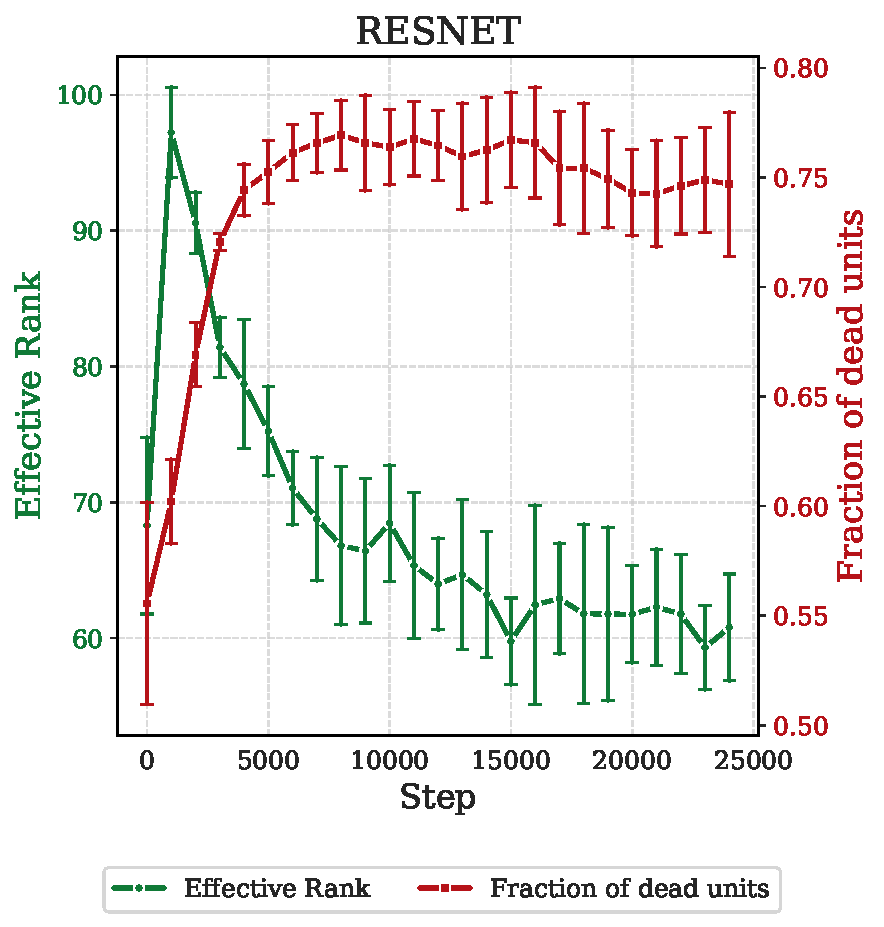
\includegraphics[width=0.24\linewidth]{paper/images/resnet_block_rankdead_plot.pdf}
    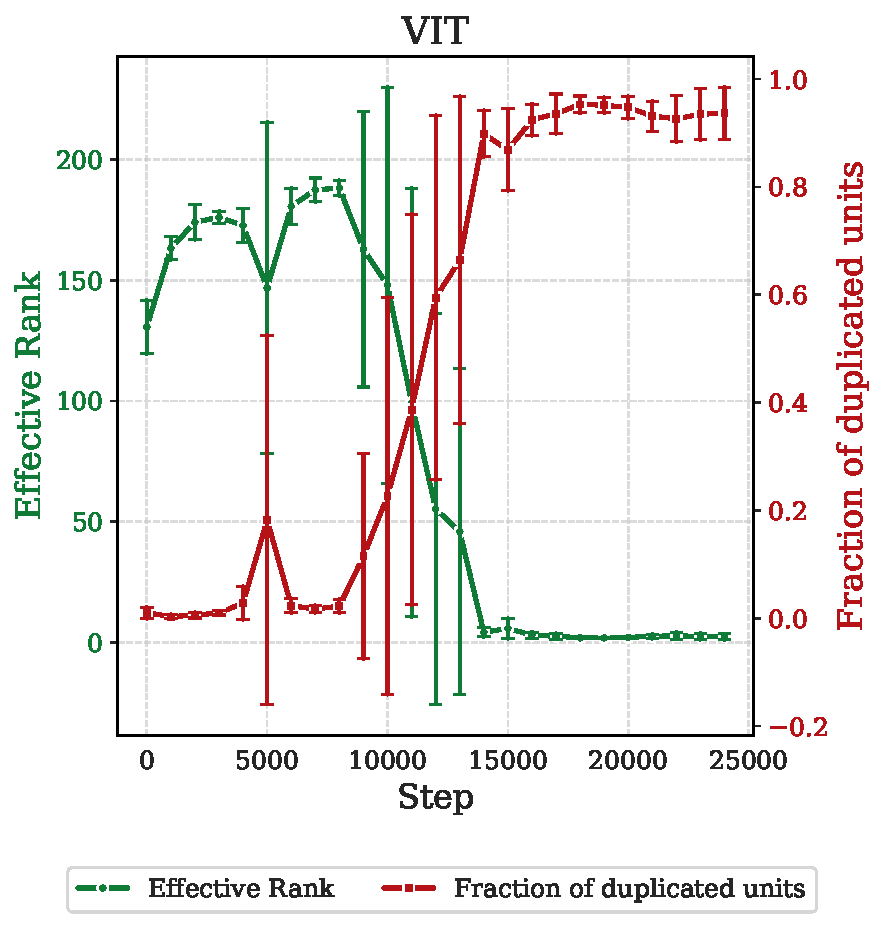
\includegraphics[width=0.24\linewidth]{paper/images/vit_block_rankdup_plot.pdf}
        \vspace{-.3cm}
    \caption{Co-evolution of Effective rank and LoP symptoms, such as dead or duplicate units in the network during continual training. (Experimental details in Appendix~\ref{app:empirical_evidence_appendix}).}
    \label{fig:norm-rank-nG}
\end{figure}
% 


Our inquiry so far highlights two key pathways to LoP common symptoms:
    (1) 
    % \GIU{The duplicate features so far have only been mentioned in passing. Should spend a sentence or two to define them above.} 
    Emergence of \textbf{duplicate features}, where distinct computational units, or groups of units, within a network layer effectively learn to become identical or highly correlated, as a potential consequence of attempting to lower representational rank, i.e.,    Remark~\ref{rem:duplicate_rank}. 
    (2) Emergence of \textbf{frozen or dead features}, where weights and biases of a unit stop learning, as a result of attempting to maximize rank increase (leading to saturation) or to flatten the loss landscape around the current parameters, i.e., Corrolary~\ref{cor:max_alpha_frozen_formal}.
Thus, the critical question now becomes: do these features, once emerged, lead to persistent LoP as defined by our framework (Definition~\ref{def:lop})? 



\section{LoP Manifolds: Traps for Gradient Descent}
% 
\AJ{do you mean the  move entire preliminary section to here or just the definitions. If we move definitions preliminary becomes one paragraph though. }
\label{sec:existence_lop_manifold}
In the previous section, we discussed how features characteristic of LoP, such as frozen units and duplicated representations, can emerge during training. Now, we formalize how these phenomena lead to the network's parameters being confined to LoP manifolds, restricting subsequent learning. We present a central proposition that jointly addresses LoP arising from frozen and duplicate units.

The intuition is that once units become unresponsive (frozen) or perfectly redundant (cloned), they tend to remain so under standard gradient-based optimization. This persistence is key to understanding LoP as a stable or semi-stable state.
\begin{proposition}
\label{prop:frozen_duplicate_lop}
Let $\theta \in \Theta$ be the parameters of a neural network.
\begin{enumerate}
    \item \textbf{Frozen Units:} Let $\theta_F$ corresponds to the incoming weights and biases of units that are consistently saturated, i.e., their activation function's derivative is zero for all inputs encountered, where $F \subset [p]$ denotes those subset of parameters, then the gradient $\nabla_{\theta_F} \Loss(\theta)$ is zero. The parameter trajectory becomes confined to a manifold $\mathcal{M}_F = \{ \theta' \in \Theta \mid \theta'_F = \theta_{F0} \}$, where $\theta_{F0}$ are the values at which saturation occurred. This is an affine LoP manifold.

    \item \textbf{Duplicate manifold:} Let us suppose we can partition the units of a network to a number of blocks, where within each block the units are perfectly cloned (i.e., they compute identical functions due to symmetric weight configurations and identical activation functions, and receive identical error signals), their  parameters of the model will be constrained such that their updates maintain this symmetry. The parameter trajectory becomes confined to an affine LoP manifold $\mathcal{M}_D$ where this symmetry is preserved (e.g., weights remain identical or maintain specific sum relations). The dimension of $\mathcal{M}_D$ is the number of connections between the partitions, which can be significantly lower than the raw parameter count.
\end{enumerate}
In both cases, the gradient $\nabla_\theta \Loss(\theta)$ is tangent to $\mathcal{M}_F$ or $\mathcal{M}_D$ respectively, satisfying Definition~\ref{def:lop}.
% 
Detailed conditions for duplicate cloning and its proof are given in  Appendix~\ref{app:cloning_manifold_details}. 
\end{proposition}

% \begin{remark}
% The LoP manifolds described in Proposition~\ref{prop:frozen_duplicate_lop} are \emph{functional}, in that they do not depend on any particular data or label distribution.\GIU{To me it seems that only condition 2 (Duplicate Units) is functional, since for frozen units there might still be a part of the input space where they activate.} For frozen units, if saturation is persistent (e.g., ReLU with consistently negative pre-activation), the zero gradient condition holds for any data. For duplicate units, if the cloning conditions on weights are met, the symmetry of activations and gradients holds for any input data and label distribution. Thus, these are functional LoP, not data-dependent ones.
% \end{remark}

\begin{remark}
The cloning LoP manifold naturally lends itself to gradient descent and stochastic gradient descent, regardless of the order which we process the samples, will remain strictly within the manifold. However, Stochastic Gradient Descent (SGD) with momentum or adaptive scaling such as Adam, or regularization techniques such as weight decay, all might violate the symmetry assumptions that were inherent to the proof of this theorem.
\end{remark}

Empirical validation of these claims, such as showing perfect cloning under specific initializations  or the persistence of dead units, can be found in Figure~\ref{fig:cloning_perfect_appendix} and Appendix~\ref{app:empirical_evidence_appendix}. One notable observation is that, despite the fact that Adam violates the symmetry conditions required for Proposition~\ref{prop:frozen_duplicate_lop}, the empirical evidence showed that it is often unable to escape the manifold nervertheless. This evidence suggests that a stronger theory might exist to explain this.


\paragraph{Stability of LoP manifolds.}
% \GIU{Added a paragraph here}
While Proposition~\ref{prop:frozen_duplicate_lop} establishes the \emph{existence} of LoP manifolds under exact conditions (perfect saturation, perfect cloning), in practice, these conditions might only be approximately reached during training. This leads to the question of whether  near-LoP states will move back closer to the LoP manifold under gradient descent dynamics, or will they move away from it. To address this, we introduce the notion of the stability of an LoP manifold.

\begin{definition}[Stability of LoP Manifold]
\label{def:lop_stability_main}
Let $\mathcal{M}$ be an LoP manifold and $N_\theta\mathcal{M}$ be the normal space to $\mathcal{M}$ at $\theta \in \mathcal{M}$. The stability of $\mathcal{M}$ is characterized by the Hessian $\nabla_\theta^2\Loss(\theta)$ in directions normal to $\mathcal{M}$:
\begin{itemize}
    \item \textbf{Stable LoP:} $\forall v\in N_\theta\mathcal{M}\setminus\{0\}: v^\top\nabla_\theta^2\Loss(\theta)v > 0$. (Perturbations revert to LoP)
    \item \textbf{Unstable LoP:} $\forall v\in N_\theta\mathcal{M}\setminus\{0\}: v^\top\nabla_\theta^2\Loss(\theta)v < 0$. (Perturbations  escape LoP)
    \item \textbf{Saddle LoP:} $\exists v_1,v_2\in N_\theta\mathcal{M}$ s.t. $v_1^\top\nabla_\theta^2\Loss v_1>0$ and $v_2^\top\nabla_\theta^2\Loss v_2<0$. (Escape is direction-dependent)
\end{itemize}
\end{definition}

\begin{remark}
Stability in the normal space to the manifold (convexity of the loss in these directions) does not imply that the loss is convex in general (i.e., also within the manifold or in other directions). These conditions are local characterizations of the loss landscape geometry around the manifold.
\end{remark}

To understand the practical implications of these stability types, consider injecting a small perturbation $\Delta\theta$ that pushes the parameters $\theta$ slightly off the manifold $\mathcal{M}$. If $\mathcal{M}$ is stable, the subsequent gradient steps $-\nabla \Loss(\theta+\Delta\theta)$ will tend to project back towards $\mathcal{M}$. If $\mathcal{M}$ is unstable, these steps will tend to move further away. For a saddle LoP manifold, escape depends on the direction of the initial perturbation relative to the eigenvectors of the Hessian in the normal space.

Therefore, the strongest form of LoP corresponds to a \emph{stable} LoP manifold, as it actively resists escape. An unstable manifold is the easiest to escape. A saddle manifold presents a mixed scenario, where random perturbations may or may not escape depending on the perturbation vector being in a positively or negative space orientation. 

\paragraph{Escaping the LoP manifolds with perturbations.}
% \GIU{I added a paragraph here}
While a full theoretical characterization of the stability of empirically observed LoP manifolds is beyond the scope of this work, our empirical investigations suggest that these manifolds are often unstable or saddle-like. This is evidenced by the fact that certain types of noise or symmetry-breaking operations can help models escape them. We highlight two common perturbations:
(1) \emph{Noisy SGD} is a modification of SGD that adds Gaussian noise to the computed gradients before parameter updates. The magnitude of this injected noise is typically proportional to the norm of the gradient, with its initial relative strength, which will decay by some factor over successive steps. By applying this noise after cloning, we can see if the model can escape the LoP manifold, or instead it will revert back to the manifold. 
% Adding noise to gradient updates (e.g., Gaussian noise $\mathcal{N}(0, \sigma^2 I)$) can push parameters off the manifold. If the manifold is unstable or saddle, subsequent noiseless steps might then lead away from it.
(2) \emph{Dropout} introduces stochasticity in the forward and backward passes by randomly zeroing activations. For cloned units, this breaks the symmetry because different clones might be active in different dropout masks, leading to divergent gradient updates. This is supported by experiments where dropout helps a model escape an artificially induced cloning manifold (see Figure~\ref{fig:dropout_escapes_cloning_appendix}).
    

\begin{figure}[!h]
    \centering
    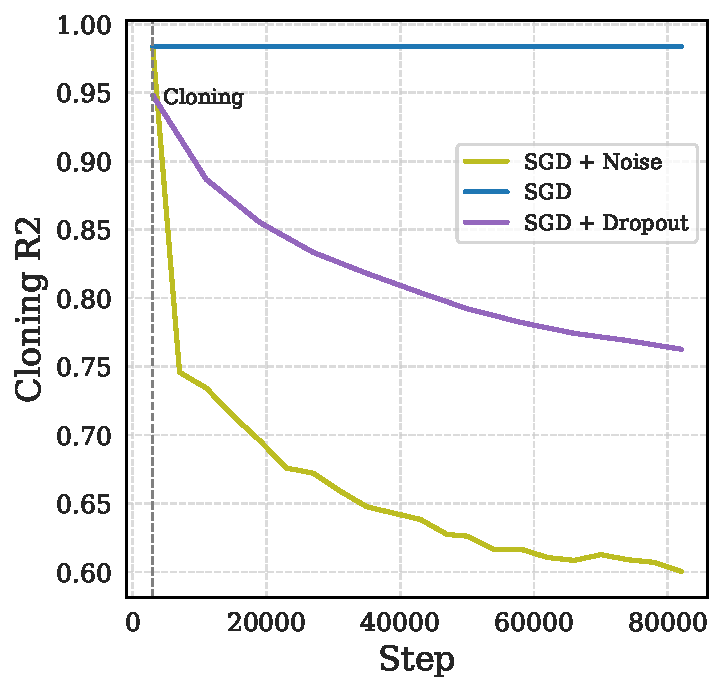
\includegraphics[width=0.24\linewidth]{cloning_R2_plot.pdf }
    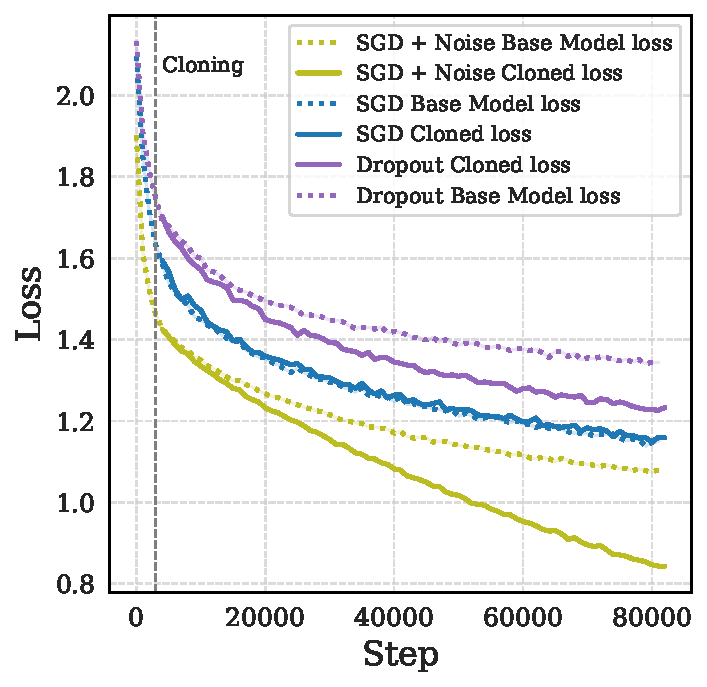
\includegraphics[width=0.24\linewidth]{cloning_losses_plot.pdf}
    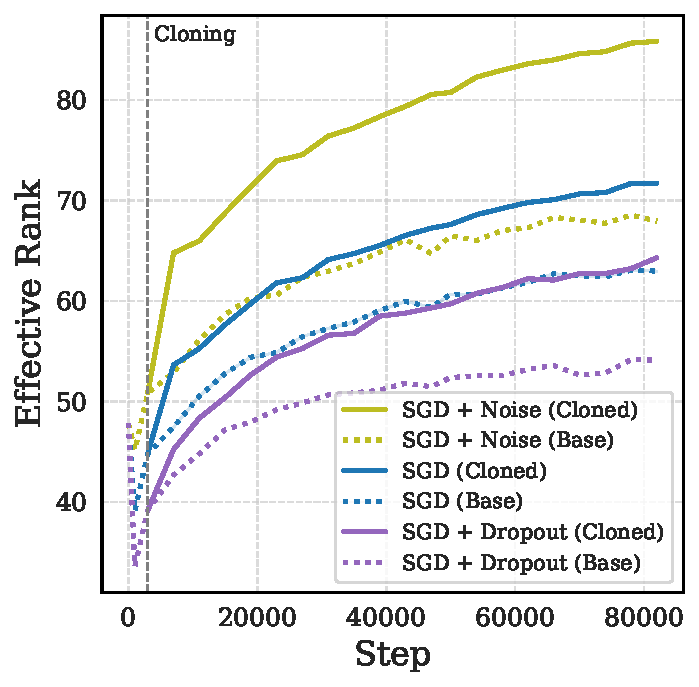
\includegraphics[width=0.24\linewidth]{cloning_rank_plot.pdf}
    \vspace{-.3cm}
    \caption{Cloning experiments on MLPs where hidden layer units are duplicated (cloning factor of 2 from a base model). 'Cloning R2 Score' (left) indicates functional identity of cloned units (higher means stronger cloning). 'Losses' (middle) compares the training loss of the cloned model ('Cloned Loss') and the original model ('Base Loss'). 'Rank' (right) refers to effective rank. The empirical data validates Proposition~\ref{prop:frozen_duplicate_lop} on duplicate manifold LoP. The cloned network dynamics remain confined in the base network manifold when using SGD, however using Noisy SGD or Dropout the dynamics can escape the manifold. (Experimental details in Appendix~\ref{app:empirical_evidence_appendix}).}
    \label{fig:enter-label} %TODO: Figure label was duplicated, consider making labels more specific if needed.
    \label{fig:cloning_perfect_appendix}
    \label{fig:dropout_escapes_cloning_appendix}
\end{figure}
% 
% 

Both noisy SGD and dropout act as symmetry-breaking operations. In the case of dropout, both forward and backward passes are asymmetric for cloned units. For noisy SGD, the backward pass (gradient update) becomes asymmetric. This asymmetry causes the parameters of notionally cloned units to slowly diverge. Remarkably, in our MLP experiments, even a small amount of gradient noise e.g., a single step with noise magnitude $0.01$ relative to gradient norms, suffices to initiate escape from an LoP manifold, though stronger noise generally leads to faster escape. In contrast, in some other settings such as Vision Transformers, while the model could escape from the manifold with a small perturbation, it did not move very far from it. More experimental studies into this direction would be vital to better understand the stability of these LoP manifolds.  


\section{Mitigation and Recovery Strategies}
\label{sec:mitigation_recovery}
\label{sec:mitigate}
Having discussed the emergence of LoP symtoms and the existence of LoP manifolds, we now turn to strategies for preventing their formation or recovering from them if they have already occurred.



\paragraph{Preventing LoP with Normalization.}
As established in Section~\ref{sec:emergence_lop}, one primary cause for activations becoming frozen is their pre-activations drifting into saturated regions. It is therefore natural to expect that normalization layers like Batch Normalization (BN) or Layer Normalization (LN) can help prevent this. By standardizing pre-activation statistics, these layers can keep activations operating in their more dynamic, non-linear range. Even with learnable affine parameters ($\gamma, \beta$) after normalization, these parameters often act to maintain pre-activations within a ``healthy'' range, rather than pushing them into extreme values that cause saturation (e.g., consistently negative for ReLU).



This is widely supported by empirical evidence (see Appendix~\ref{app:empirical_evidence_appendix}, Figures like \ref{fig:emergence_lop_symptoms_cl} in Section~\ref{sec:emergence_lop}, and Figure~\ref{fig:normalizations-recovering} below). BN and LN generally help maintain higher effective rank of representations throughout training (as seen in Figure~\ref{fig:norm-rank-nG}) and concurrently prevent frozen/dead features and excessive feature duplication from becoming dominant.


\begin{figure}[h!]
    \centering
    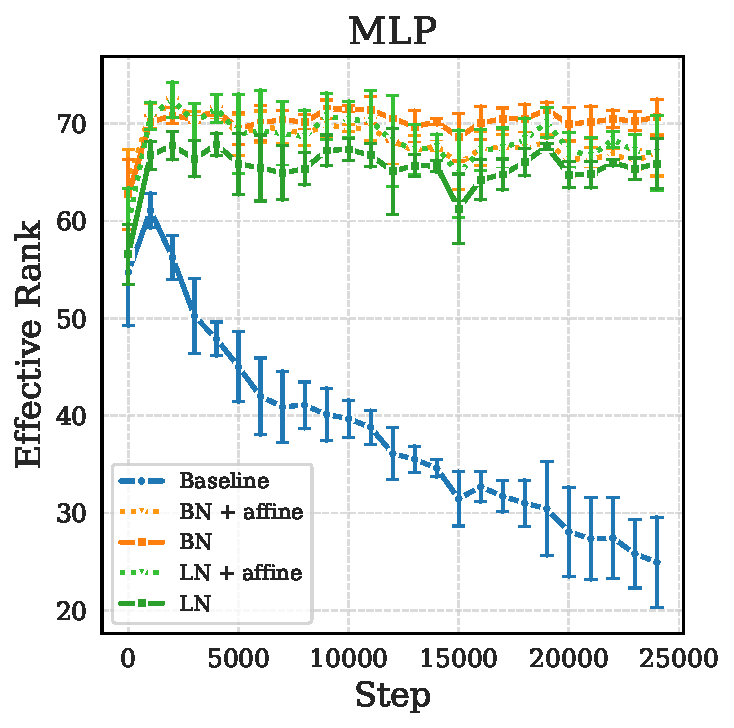
\includegraphics[width=0.24\linewidth]{paper/images/mlp_act__eff_rank_normalizations_plot.pdf}
    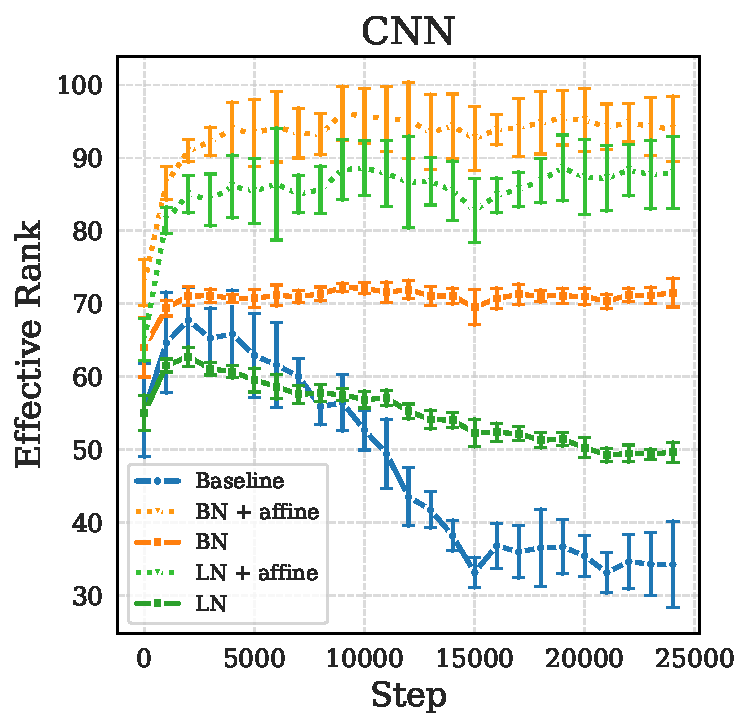
\includegraphics[width=0.24\linewidth]{paper/images/cnn_act__eff_rank_normalizations_plot.pdf}
    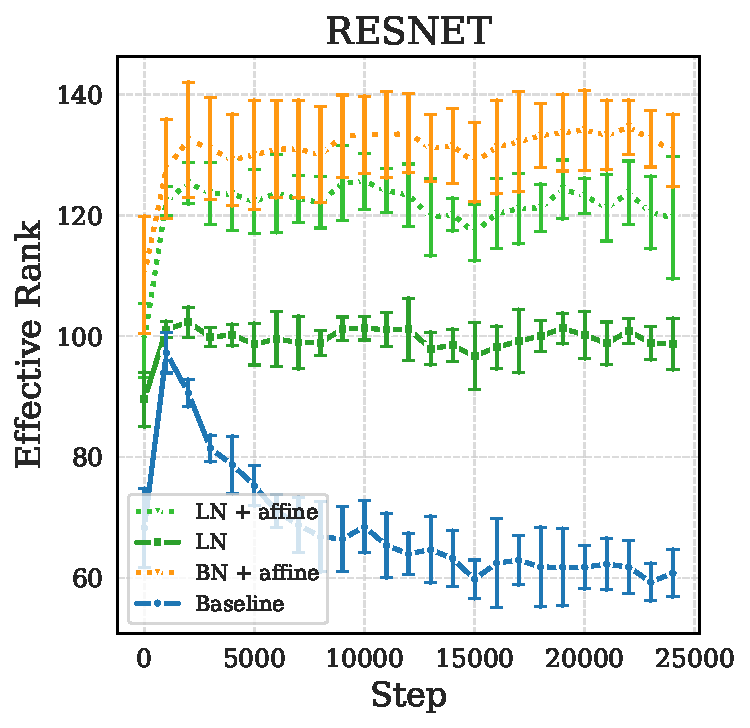
\includegraphics[width=0.24\linewidth]{paper/images/resnet_block_eff_rank_normalizations_plot.pdf}
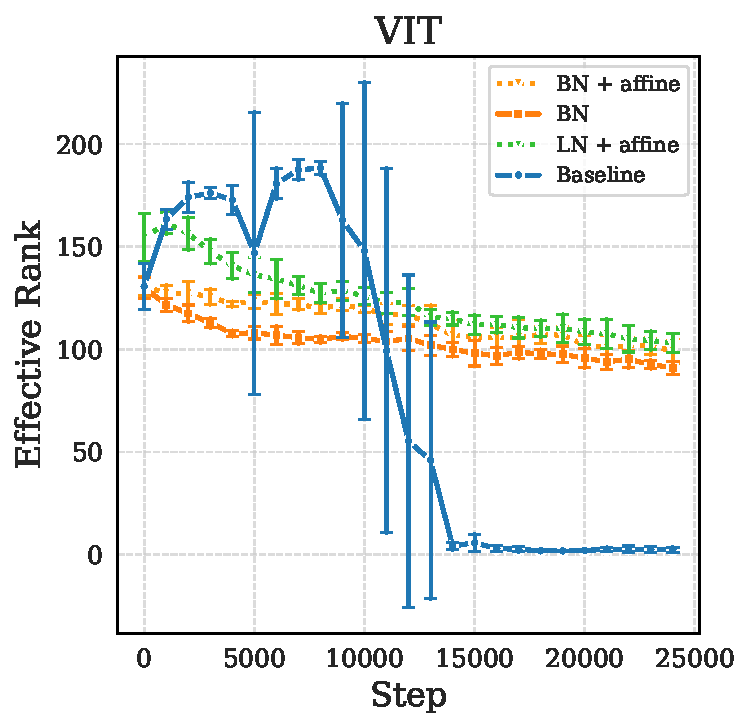
\includegraphics[width=0.24\linewidth]{paper/images/vit_block_eff_rank_normalizations_plot.pdf}
    
    \caption{Evolution of the Effective rank during training for architectures with and without normalization layers. Dotted lines represent normalization with affine parameters. (Experimental details in Appendix~\ref{app:empirical_evidence_appendix}).}
    \label{fig:norm-rank}
\end{figure}



\paragraph{Recovery from LoP via Perturbations.}
What if LoP conditions, such as widespread frozen units or extensive feature cloning, have already set in? In such cases, mitigation strategies like normalization, which act proactively, may no longer be sufficient to reverse the state, as indicated by cloning experiments where normalization alone doesn't break perfect, established clones. However, similar to our discussion on manifold stability (Section~\ref{sec:existence_lop_manifold}), injecting noise into the training process can be a viable recovery strategy.

The principle is that if the LoP manifold is unstable or saddle-like, perturbations can allow the optimizer to find an escape route. Noisy SGD and the more sophisticated Continual Backpropagation \citep{dohare2024loss} are examples of such mechanisms. An interesting benchmark are the ``bit-flipping'' experiments, a regression task where the current sample is a stochastic function of the previous sample (see \citep{dohare2024loss} and Appendix~\ref{app:empirical_evidence_appendix} for full details). In this setup, a target network uses Linear Threshold Units (LTUs), and the input consists of $m$ bits, $f$ of which periodically flip their state, creating a non-stationary target function that a two-layer MLP is trained online to learn. The model size is controlled to be lower than the complexity of the data generating function. Figures~\ref{fig:CBP-scale-rank} and \ref{fig:CBP-scale-dup} illustrate how aspects like rank and feature duplication are affected by the perturbed dynamics and the dimensionality of the model.    Illustrations of recovery dynamics can be found in Appendix~\ref{app:empirical_evidence_appendix}.
\begin{figure}[!ht]
    \centering
    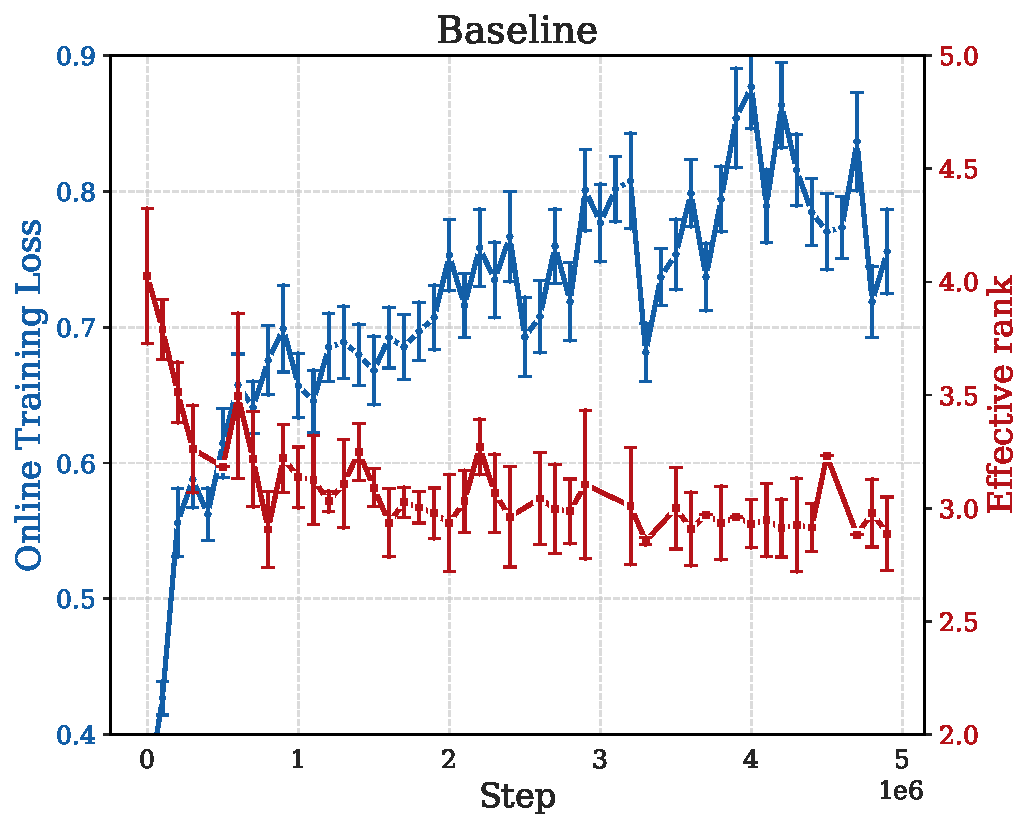
\includegraphics[width=0.33\linewidth]{paper/images/bf_Baseline_rankloss_plot.pdf}
    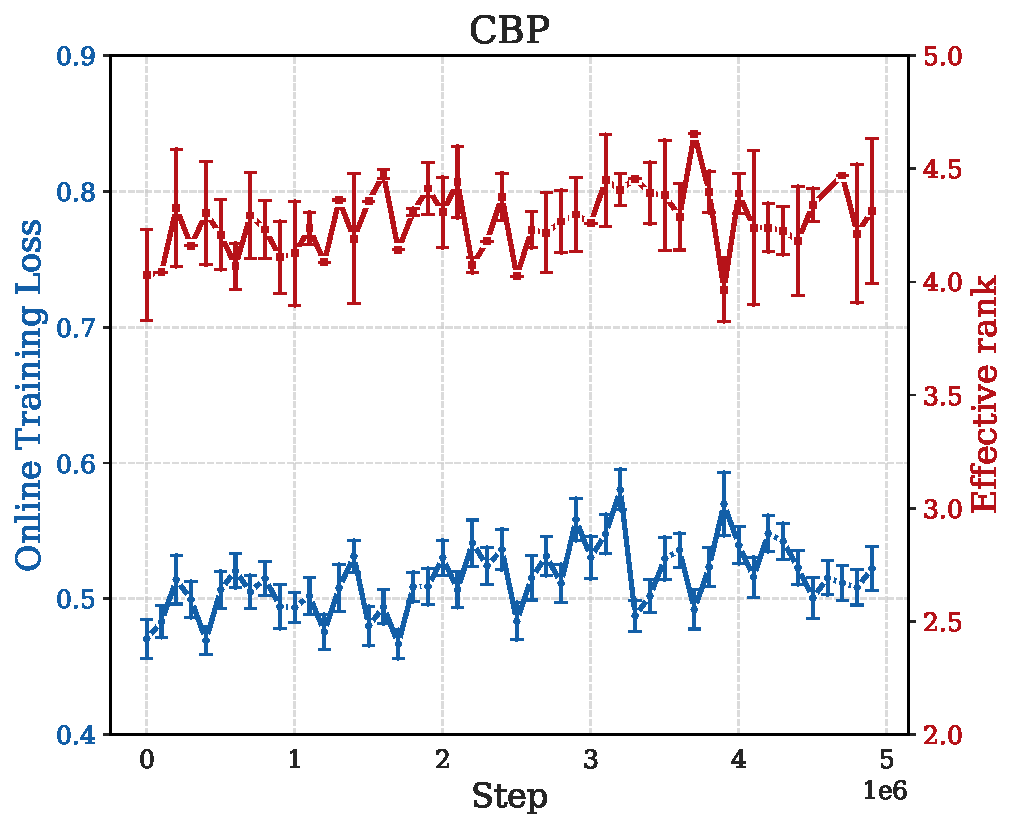
\includegraphics[width=0.33\linewidth]{paper/images/bf_CBP_rankloss_plot.pdf}
        \vspace{-.3cm}
    \caption{Bit Flipping experiment on 5M samples. Low rank structures emerge during training with standard Backpropagation (BP) while the rank remains stable with Continual Backpropagation (CBP), suggesting CBP helps maintain representational diversity. (Experimental details in Appendix~\ref{app:empirical_evidence_appendix}).}
    \label{fig:CBP-scale-rank}
\end{figure}
\begin{figure}[!ht]
    \centering
    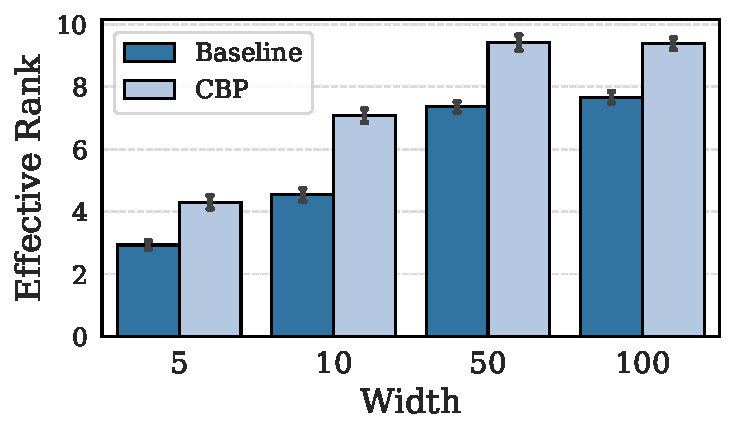
\includegraphics[width=0.23\linewidth]{paper/images/bf_Effective Rank_CBP_barplot.pdf}
    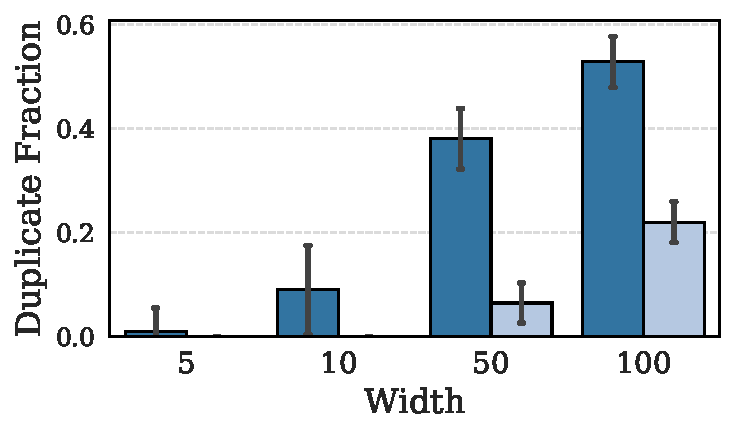
\includegraphics[width=0.23\linewidth]{paper/images/bf_Duplicate Fraction_CBP_barplot.pdf}
    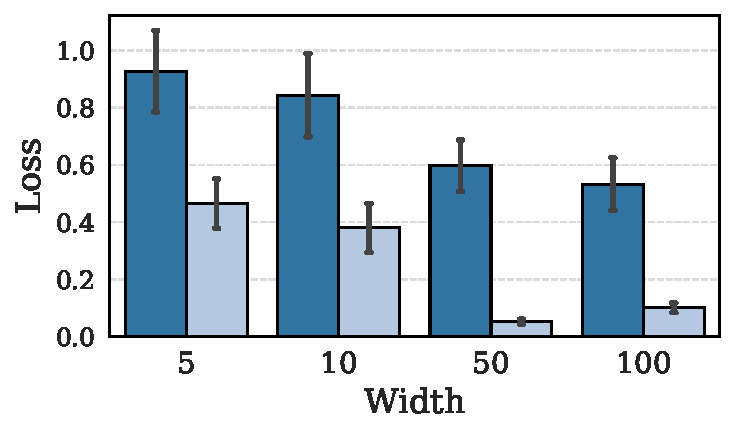
\includegraphics[width=0.23\linewidth]{paper/images/bf_Loss_CBP_barplot.pdf}
    \vspace{-.3cm}
    \caption{Bit Flipping experiment on 5M samples. Duplicated structures (indicated by fraction of duplicate features at different layers/scales) emerge during training with standard Backpropagation (BP) but are less prevalent with Continual Backpropagation (CBP). As the model width is increased more duplicate features emerge. The size of the data generating function is $100$. (Other experimental details in Appendix~\ref{app:empirical_evidence_appendix}).}
    \label{fig:CBP-scale-dup}
\end{figure}
% 

An interesting distinction arises when comparing artificially induced LoP (like explicit cloning) with naturally emerging LoP symtoms in challenging scenarios like continual learning. In controlled cloning setups (e.g., as conceptualized in Figure~\ref{fig:dropout_escapes_cloning_appendix}, dropout can be effective in breaking the artificially imposed symmetry and allowing units to diverge. In contrast, in our continual Bit Flipping experiments, the role of dropout can be mixed or even detrimental. While it might prevent some forms of LoP, it can also hinder the consolidation of new knowledge or exacerbate forgetting if it too aggressively discards learned information relevant to the new task. This suggests that the optimal strategy for maintaining or recovering plasticity might be context-dependent.


\section{Conclusion}
\label{sec:discussion}
% \IMZ{Don't forget to add the NeurIPS checklist after the references!}
This work has presented a mathematical framework to understand Loss of Plasticity (LoP) in deep neural networks through the lens of dynamical systems. We formally defined LoP manifolds as regions in parameter space that trap gradient-based optimization, and identified two primary mechanisms for their formation: the saturation of activations leading to \emph{frozen units}, and representational redundancy manifesting as \emph{cloned-unit manifolds}. Our analysis highlights that these LoP states are often characterized by a reduction in the effective rank of representations. We explored how architectural choices like normalization can mitigate the emergence of LoP, and how perturbations such as noise injection can facilitate escape from these restrictive manifolds, depending on their stability.

A key insight from our investigation is the inherent tension between learning objectives in static versus dynamic environments. Properties conducive to good generalization on a fixed dataset, such as the emergence of low-rank features or simplicity biases, appear to be the very same properties that can lead to a loss of adaptability when the learning process is extended over time or across changing tasks. This suggests that continual learning requires mechanisms that actively preserve or regenerate representational diversity.

Several open questions and directions for future research emerge from this study.
From a theoretical standpoint, our analysis has primarily focused on linear or affine LoP manifolds. Do non-linear LoP manifolds exist, and could they emerge in practical network training? Further, a more comprehensive theoretical understanding of the stability conditions (stable, unstable, or saddle) for various types of LoP manifolds is needed. What are the precise architectural or data conditions that lead to one type of stability over another? 
% \GIU{Do we have numbers proving this?}\AJ{this is the open questions section, isn't natural that we don't knwo all the answers here?}\GIU{Of course, but the way it is said now appears like we  know this for a fact.} 
Numerically, the curvature of the loss landscape in directions normal to an LoP manifold is critical. Even for an unstable manifold, if the negative curvatures are very slight (near flat), escaping might require significant perturbations or many training steps. Characterizing these curvatures and their impact on escape dynamics would be valuable.

While we have shown that models can escape artificially cloned LoP manifolds with interventions like dropout or noise, it remains an open question whether a model, once recovered from such a state, can explore the parameter space as effectively and find solutions as generalizable as a model trained from a fresh, random initialization. The question of whether we can fully restore exploratory capacity after falling into a highly restricted subspace is of significant practical importance.

One of the most intriguing outcomes of this work is the connection established between the phenomenon of unit cloning (often studied in model compression or network analysis) and LoP in continual learning. These have largely been treated as separate fields of inquiry. Our theoretical framework, particularly the propositions regarding cloned units, reveals a deep link, suggesting that insights and tools can be transferred between these domains.  This prompts questions like whether techniques from continual learning, such as noisy backpropagation or methods like Continual Backpropagation (CBP) \citep{dohare2024loss}, could be beneficial in the context of model expansion or escaping cloned states in other scenarios.

Ultimately, understanding and overcoming LoP is crucial for building AI systems that can learn continuously and adapt robustly in an ever-changing world. By providing a mathematical characterization of some fundamental barriers to such adaptation, we hope this work paves the way for the development of new architectures and learning algorithms that can sustain plasticity indefinitely, leading to truly lifelong learning agents.

\bibliography{refs}

% \section*{NeurIPS Paper Checklist}
% \begin{enumerate}
% \item {\bf Claims}
%       \item Answer: \answerYes{}
%       \item Justification: The claims in the abstract and introduction accurately reflect the paper's contributions on LoP in neural networks, linking it to specific mechanisms (saturation, cloning) and proposing a dynamical systems framework.

% \item {\bf Limitations}
%       \item Answer: \answerYes{}
%       \item Justification: Limitations are discussed in the Discussion section (Section 6), acknowledging open questions regarding non-linear manifolds, lack of our theoretical understanding of stability of LoP manifolds, effect of momentum and adaptive scaling, and the need for more sophisticated continual randomization schemes.

% \item {\bf Theory assumptions and proofs}
%       \item Answer: \answerYes{}
%       \item Justification: All theoretical results (propositions, corollary) state their assumptions clearly. Complete proofs are provided in Appendix~\ref{app:theory_appendix}.

% \item {\bf Experimental result reproducibility}
%       \item Answer: \answerYes{} % Changed from Yes to NA as experiments are planned
%       \item Justification: Section~\ref{app:empirical_evidence_appendix} outlines all experiments. Details on specific datasets, architectures, hyperparameters, and evaluation protocols would be provided with the results in a final version, enabling reproducibility. Code would also be released.

% \item {\bf Open access to data and code}
%       \item Answer: \answerYes{} % Changed from Yes to NA as experiments are planned
%       \item Justification: Code and experimental configurations related to experiments the paper, in particular extensively discussed in Section~\ref{app:empirical_evidence_appendix} will be made available upon completion and acceptance. Only standard datasets (e.g., CIFAR, ImageNet variants) will are used.

% \item {\bf Experimental setting/details}
%       \item Answer: \answerYes{} % Changed from Yes to NA
%       \item Justification: Section~\ref{app:empirical_evidence_appendix} provides a detailed experimental settings (architectures, optimizers, learning rates, task sequences, specific metrics implementations) will be included when reporting results.

% \item {\bf Experiment statistical significance}
%       \item Answer: \answerYes{} % Changed from Yes to NA
%       \item Justification: Methods for ensuring statistical significance, we used multiple multiple runs with different random seeds (ranging between 3 and 5) for each of the points on our experimental grid, reporting means and standard deviations/errors), in order present the results throughout the paper and detailed in  Section~\ref{app:empirical_evidence_appendix}.

% \item {\bf Experiments compute resources}
%       \item Answer: \answerNo{}
%       \item Justification: Details about computational resources (e.g., GPU types, number, training times) for the finalised experiments, which include those that appear in the appendix only, will be added in the final version presenting the empirical results.

% \item {\bf Code of ethics}
%       \item Answer: \answerYes{}
%       \item Justification: The research aims to understand fundamental AI capabilities and limitations, adhering to ethical research practices. It does not involve sensitive data or high-risk applications directly. Conforms to the NeurIPS Code of Ethics.

% \item {\bf Broader impacts}
%       \item Answer: \answerNA{}
%       \item Justification: This is a foundational research paper and not directly linked to any specific application. 

% \item {\bf Safeguards}
%       \item Answer: \answerNA{}
%       \item Justification: This paper presents a theoretical framework and planned experiments. It does not release new models or datasets with immediate potential for misuse. Safeguards related to potential future applications are discussed in the Broader Impacts section.

% \item {\bf Licenses for existing assets}
%       \item Answer: \answerNA{} % Changed from Yes to NA
%       \item Justification: The  experiments use standard, publicly available datasets (e.g., CIFAR, ImageNet) which have permissive licenses for research use.

% \item {\bf New assets}
%       \item Answer: \answerNA{} % Changed from Yes to NA
%       \item Justification: Code developed for the experiments will be released with appropriate documentation and an open-source license upon publication.

% \item {\bf Crowdsourcing and research with human subjects}
%       \item Answer: \answerNA{}
%       \item Justification: This research is purely theoretical and computational, involving no human subjects or crowdsourcing.

% \item {\bf Institutional review board (IRB) approvals or equivalent for research with human subjects}
%       \item Answer: \answerNA{}
%       \item Justification: Not applicable as no human subjects are involved.

% \item {\bf Declaration of LLM usage}
%       \item Answer: \answerNo{}
%       \item Justification: No LLMs were used in the development of the core theoretical analyses or development of experiments presented in this research. 
% \end{enumerate}

% \renewcommand{\thefigure}{\thesection.\arabic{figure}}


\appendix
% \newpage

\section{Theoretical Appendix}
% 
\label{app:theory_appendix}
This section contains detailed proofs of propositions and lemmas, further theoretical derivations, and discussions extending the concepts presented in the main paper. 

\subsection{Rank recovery with non-linear activations}

In the present section, hard rank refers to the number of independent linear components of a matrix (rows or columns), which is an integer between $1$ and the minimum of number of rows and columns. Full rank implies that this number for a matrix matches its theoretical maximum, and rank-deficient means the opposite. However, this number is not suitable in empirical settings where a small noise to a rank-deficient matrix might make it appear full-rank. To alleviate this, we use effective rank, which provides a numerically amenable analogue. For a positive definite $n\times n$ matrix $C$ with eigenvalues $\lambda_1,\dots, \lambda_n,$ effective rank is defined as 
\begin{align*}
&\tilde{r}(C)= \exp(H) &&H =-\sum_i^n p_i\log p_i &&&  p_i = \frac{\lambda_i}{\sum_{k=1}^n \lambda_k}.
\end{align*}

Recall the definition of pre-activations matrix $X \in \R^{n \times d}$ ($n$ samples, $d$ features with $n\ge d$), defined as each row is independently drawn from a multivariate Gaussian distribution $\mathcal{N}(0, C)$, with $C$ being the covariance matrix that has unit diagonals, off-diagonals strictly in $(-1,1)$. We also defined post-activation covariance $C_f = \frac1n \E f(X)^\top f(X).$ Let us re-state the proposition:

\begin{proposition}[Rank recovery with non-linear activations (re-stated Proposition~\ref{prop:rank_recovery_informal})]
Let us assume that  $f$ is not a bounded degree polynomial, and that $\E f(z)^2,$ where $z\sim N(0,1),$ is bounded. First, $C_f$ has full rank (hard rank), even if the input features $X$ is rank-deficient. Second, if the input features are highly correlated with effective rank $1+\epsilon$ for some small constant $\epsilon>0,$ effective rank of $C_f$ will be approximately  $1 + \alpha_f \epsilon,$ with the coefficient defined as $\alpha_f = \frac{\E f'(z)^2}{\E f(z)^2 } - 1$ with $z\sim N(0,1).$
\end{proposition}
% \AJ{It's kind of hard to replace the label A.1 with 3.1 and might be a bit messy, I just added some clarification, is it sufficient?}

First, observe that because each row is iid, we can also write the expected post-activation covariance based on a single sample $C_f = \E f(X) f(X)^\top,$ where elements of $x$ are standard Gaussian with covariance $\E X_i X_j = C_{ij}. $ This will streamline the proof of this proposition.  We can break this proposition into two parts: the claim on hard rank recovery and the claim on the effective rank, which will be given separately in the subsequent parts. 


\subsubsection*{Hard rank recovery}

\begin{proposition}
\label{prop:rank}
Let $f:\R\to\R$ be non-linear activation that is not a bounded degree polynomial and is square-integrable with respect to the Gaussian kernel $\mathcal{N}(0,1)$. Consider a vector of pre-activations $z\in\R^d$ whose components are jointly Gaussian, $z \sim \mathcal{N}(0, \Sigma)$, with covariance matrix $\Sigma$ such that $\E[z_i z_j]=\Sigma_{ij}$ and $|\Sigma_{ij}|<1$ for $i \neq j$ (assuming unit variance for simplicity, $\Sigma_{ii}=1$). Then the covariance matrix of the post-activations $C = \E[f(z)f(z)^\top]$ is full rank, unless some features are perfectly correlated or anti-correlated (i.e., $|\Sigma_{ij}|=1$) or are exact duplicates.
\end{proposition}

\begin{proof} Let $f:\R\to\R$ be square-integrable w.r.t. $\gamma = \mathcal{N}(0,1)$ and not a polynomial. Let $z \sim \mathcal{N}(0, \Sigma)$ with $\Sigma_{ii}=1$ and $|\Sigma_{ij}| < 1$ for $i \neq j$. We want to show $C = \E[f(z)f(z)^\top]$ is full rank.
    Since $f$ is square-integrable w.r.t. $\gamma$, it has a Hermite expansion $f(x) = \sum_{k=0}^{\infty} b_k \frac{\He_k(x)}{\sqrt{k!}}$, where $\He_k(x)$ are the standard probabilist's Hermite polynomials and $b_k = \E[f(Z) \frac{\He_k(Z)}{\sqrt{k!}}]$ for $Z \sim \mathcal{N}(0,1)$. Since $f$ is not a polynomial, infinitely many $b_k$ must be non-zero. For simplicity, let's use the physicist's convention where $f(x) = \sum_{k=0}^{\infty} c_k \He_k(x)$ with $c_k = \frac{1}{2^k k! \sqrt{\pi}} \int f(x) \He_k(x) e^{-x^2} dx$. Infinitely many $c_k$ are non-zero.

    Mehler's formula \citep{mehler1866ueber, erdelyi1953higher} provides the expectation of products of Hermite polynomials for correlated Gaussian variables. For $(Z_i, Z_j)$ jointly Gaussian with mean 0, variance 1, and correlation $\rho = \Sigma_{ij}$, we have $\E[\He_k(Z_i) \He_l(Z_j)] = \delta_{kl} 2^k k! \rho^k$.

    The $(i, j)$-th entry of the covariance matrix $C$ is $C_{ij} = \E[f(z_i) f(z_j)]$. Substituting the Hermite expansion:
    \begin{align*}
    C_{ij} &= \E\left[ \left( \sum_{k=0}^{\infty} c_k \He_k(z_i) \right) \left( \sum_{l=0}^{\infty} c_l \He_l(z_j) \right) \right] \\
    &= \sum_{k=0}^{\infty} \sum_{l=0}^{\infty} c_k c_l \E[\He_k(z_i) \He_l(z_j)] \\
    &= \sum_{k=0}^{\infty} c_k^2 \E[\He_k(z_i) \He_k(z_j)] \quad (\text{using orthogonality } \delta_{kl}) \\
    &= \sum_{k=0}^{\infty} c_k^2 (2^k k!) (\Sigma_{ij})^k
    \end{align*}
    Let $a_k = c_k^2 (2^k k!)$. Since infinitely many $c_k \neq 0$, infinitely many $a_k > 0$. The matrix $C$ can be written as $C = \sum_{k=0}^{\infty} a_k \Sigma^{\odot k}$, where $\Sigma^{\odot k}$ is the element-wise $k$-th power (Hadamard power) of the pre-activation covariance matrix $\Sigma$.

    We know $\Sigma$ is positive semidefinite (as it's a covariance matrix) and by assumption $\Sigma_{ii}=1$ and $|\Sigma_{ij}|<1$ for $i \neq j$. $\Sigma^{\odot 0}$ is a matrix of all ones (rank 1). $\Sigma^{\odot 1} = \Sigma$. For $k \ge 1$, if $\Sigma$ is positive definite, then $\Sigma^{\odot k}$ is also positive definite (Schur product theorem). Even if $\Sigma$ is only positive semidefinite, as $k$ increases, the off-diagonal elements $(\Sigma_{ij})^k$ decay towards zero since $|\Sigma_{ij}|<1$. By Gershgorin circle theorem arguments, for large enough $k$, the matrix $\Sigma^{\odot k}$ becomes strictly diagonally dominant and thus positive definite, provided $\Sigma$ doesn't represent linearly dependent variables (which is implied by $|\Sigma_{ij}|<1$).

    Since $C$ is a sum of positive semidefinite matrices ($\Sigma^{\odot k}$ for $k \ge 1$, scaled by non-negative $a_k$), and at least one $a_k > 0$ corresponds to a positive definite $\Sigma^{\odot k}$ (for $k \ge 1$, assuming $\Sigma$ is not degenerate), the resulting matrix $C$ will be positive definite, hence full rank. The only exception is if the original $z_i$ were linearly dependent such that $\Sigma$ was rank-deficient in a way that persists through the Hadamard powers (e.g., if $z_i = z_j$ or $z_i = -z_j$, making $\Sigma_{ij}=1$ or $\Sigma_{ij}=-1$, violating the assumption).
\end{proof}


\subsubsection*{Effective rank recovery}

Here, let us assume that the covariance matrix has unit diagonals and highly correlated features. 

\begin{lemma}
    If $X,Y \sim N(0,1)$ are nearly identical $\E X Y = 1- \epsilon,$ for some small $\epsilon, $ then the post activations will satisfy 
    \[
    \frac{\E f(X)f(Y)}{\sqrt{\E f(X)^2 \E f(Y)^2}}  \approx 1 - (\alpha_f + 1) \epsilon.
    \]
\end{lemma}

We can prove a more quantitative version of rank recovery via our notion of effective rank: 

\begin{proposition}
Let us consider pre-activations that are highly correlated $C_{ij} = 1-\epsilon,\forall i\neq j,$ for some small $\epsilon, $  which is approximate a rank-1 matrix. For sufficiently small $\epsilon$ and sufficiently large $n,$ the post-activation effective rank will be approximately 
    \begin{align*}
    \tilde{r}(C_f)\approx \tilde{r}(C)(1 + \alpha_f \epsilon \ln(n/\epsilon) )
\end{align*}
\end{proposition}

\begin{proof}
    The first lemma is that the activation can de-correlate these features effectively. 
Thus, if we normalized post activations by $\E f(z)^2 $ where $z\sim N(0,1),$ resulting normalized post-covariance $\widetilde{C}_f = C_f / \E f(z)^2$ will have unit diagonals and off-diagonals equal to $1-(\alpha_f + 1) \epsilon.$ 

Now, a fact from linear algebra is that matrix $C$ will have top eigenvalue $1+(n-1)(1-\epsilon)$ and $n-1$ smaller eigenvalues $\epsilon. $ Thus, for sufficiently large $n$ we can approximate its effective rank as:
\begin{align*}
    p_1 \approx 1-\epsilon,\;  
    p_2,\dots, p_n \approx \epsilon/n \implies H(C)=-\sum_k p_k\ln p_k \approx \epsilon\ln(ne/\epsilon)
\end{align*}

Now, notice that $\widetilde{C}_f$ is similar in structure to $C,$ if we replace $\epsilon$ by $(1+\alpha_f)\epsilon. $ If we replace these into the effective rank definition we will have the first order approximation to the new effective rank:

\begin{align*}
    \tilde{r}(C_f)\approx \tilde{r}(C)(1 + \alpha_f \epsilon \ln(n/\epsilon) )
\end{align*}
Where we now replaced $\widetilde{C}_f$ by $C_f$ instead the effective rank because effective rank is scale-free, this scaling will not change its effective rank.  

\end{proof}


\subsubsection{Maximizing Rank Recovery Leads to Frozen Activations}
\label{app:max_rank_frozen}

In this section, we provide a detailed analysis of how attempts to maximize the rank recovery strength $\alpha_f$ through manipulation of pre-activation statistics can paradoxically lead to frozen units with near-zero gradients. This phenomenon, briefly mentioned in Corollary~\ref{cor:max_alpha_frozen_formal} of the main text, represents a fundamental trade-off in neural network optimization. We will show this corrolary in a particular parameterization of the activation where we manipulate it by shifting and sscaling the pre-activation. 

Consider an  activation function $f: \mathbb{R} \to \mathbb{R}$ and its manipulated version through pre-activation transformations:
$$f_{a,b}(z) = f(az + b)$$
where $a > 0$ represents scaling and $b \in \mathbb{R}$ represents shifting. For $z \sim \mathcal{N}(0,1)$, the rank recovery strength of this manipulated activation is:
$$\alpha_{f_{a,b}} = \frac{\mathbb{E}[f'_{a,b}(z)^2]}{\mathbb{E}[f_{a,b}(z)^2]} - 1$$


Let us assume $f:\mathbb{R}\to\mathbb{R}$ to be a continuous, piecewise smooth function satisfying one of the following conditions:
\begin{enumerate}
    \item \emph{Half-vanishing, half-growth:} For some $p > 1/2$, On one side (say $x \geq 0$): $f(x) = x^p(1 + O(1/|x|))$ and $f'(x) = px^{p-1} (1+O(1/|x|)),$ and on the other side ($x < 0$): $f(x) = O(1/|x|)$ and $f'(x) = O(1/|x|^2)$
    For these functions, $\alpha_{f_{a_k,b_k}}$ becomes unbounded roughly as $(b_k/a_k)^2$ in the limit of $(a_k,b_k) $ growing very large, negative shift $b_k < 0$, and scale grows slower than shift magnitude $\lim_{k\to\infty} a_k/b_k \to 0^-$. 
    
    \item \emph{Plateauing on both sides:} We have $\lim_{x \to \pm\infty} f(x) = C_{\pm}$ (finite constants) and $|f'(x)| = O(1/x^2)$ as $x \to \pm\infty.$
    For these functions, $\alpha_{f_{a_k,b_k}}$ grows unbounded roughly as $a_k$ when $a_k$ grow unbounded as $k$ grows, and scale not growing slower than shift $\lim_{k\to\infty} a_k/b_k \neq 0 .$
\end{enumerate}

The given sequences $(a_k, b_k)$  will lead to $\alpha_{f_{a_k,b_k}} \to \infty$ in the limit when $k$ grows, and the limiting manipulated function has zero derivative almost everywhere with respect to the Gaussian measure. Specifically, for any $\epsilon > 0$:
$$\lim_{k \to \infty} \mathbb{P}(f'_{a_k,b_k}(z) < \epsilon) = 1 \quad \text{for } z \sim \mathcal{N}(0,1)$$

\begin{remark}
Most commonly used activation functions fall into one of these categories:
\begin{itemize}
    \item \emph{Half-vanishing half-growth:} ReLU, ELU, SELU, GELU, Swish, Softplus
    \item \emph{Plateauing on both sides:} Tanh, Sigmoid, Softsign
\end{itemize}
Notable exceptions include LeakyReLU and parametric ReLU variants that maintain non-zero slopes on both sides.
\end{remark}


% \subsubsection{Intuition and Examples}

The key insight is that maximizing rank recovery strength requires pushing the activation function into extreme operating regimes:

\begin{example}[Tanh Activation]
For $f(x) = \tanh(x)$ and the manipulated version $f_{a,0}(z) = \tanh(az)$:
\begin{itemize}
    \item As $a \to \infty$: $f_{a,0}(z) \to \text{sign}(z)$
    \item The derivative $f'_{a,0}(z) = a \cdot \text{sech}^2(az) \to 0$ for all $z \neq 0$
    \item This achieves maximal rank recovery ($\alpha \to \infty$) but completely freezes gradient flow
\end{itemize}
\end{example}

\begin{example}[ReLU Activation]
For $f(x) = \text{ReLU}(x) = \max(0, x)$ and $f_{a,b}(z) = \text{ReLU}(az + b)$:
\begin{itemize}
    \item To maximize $\alpha$: need $b < 0$ and $|b|/a \to \infty$
    \item This shifts most pre-activations below zero: $\mathbb{P}(az + b < 0) \to 1$
    \item Results in dead ReLU units with $f'_{a,b}(z) = 0$ for almost all $z$
\end{itemize}
\end{example}

\subsubsection{Numerical Validations of Activation Function Theory}
\label{app:numerical_validations_activations}

In this section, we present comprehensive numerical validations of our theoretical results regarding activation functions, rank recovery, and the emergence of frozen states. These experiments directly validate Proposition~\ref{prop:rank_recovery_informal} on rank recovery and Corollary~\ref{cor:max_alpha_frozen_formal} on the emergence of frozen units. All figures produced here can be reproduced by running \texttt{theory.py} script. 

\paragraph{Validation 1: Hard Rank Recovery from Rank-Deficient Inputs.}
Figure~\ref{fig:validation_hard_rank_recovery} demonstrates that non-linear activation functions can indeed recover full rank from rank-deficient pre-activations, validating the theoretical claims in Proposition~\ref{prop:hard_rank_increase_main}.

\begin{figure}[ht!]
    \centering
    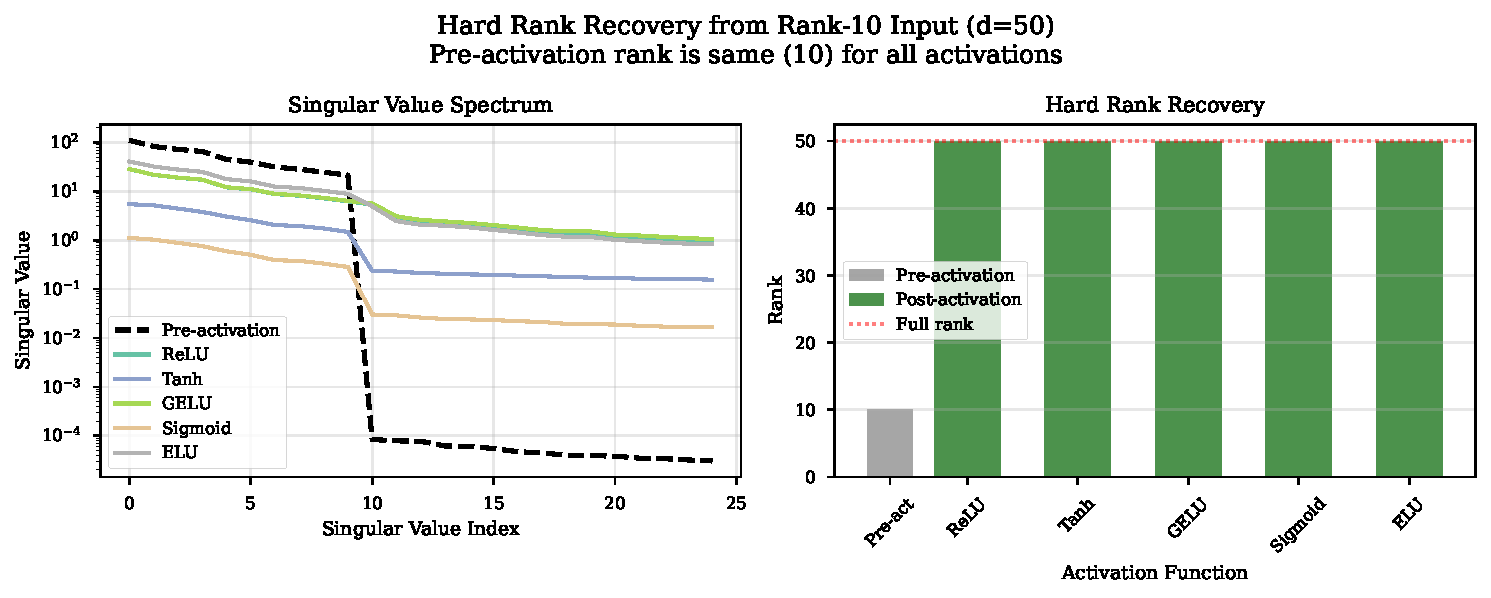
\includegraphics[width=0.9\linewidth]{validation_hard_rank_recovery.pdf}
    \caption{Validation of hard rank recovery through non-linear activations. \textbf{Left:} Singular value spectrum showing how different activation functions (ReLU, Tanh, GELU, Sigmoid, ELU) transform the singular values of rank-deficient input data (rank-10 in 50-dimensional space). The black dashed line shows the pre-activation spectrum with clear rank deficiency. All non-linear activations expand the spectrum, recovering higher ranks. \textbf{Right:} Comparison of pre- and post-activation ranks across activation functions. The gray bars show the input rank (10), while green bars show the recovered rank after activation. All tested activations achieve substantial rank recovery, with some recovering nearly full rank (50), confirming that non-linearities counteract the rank-reducing effects of linear transformations as discussed in Section~\ref{sec:emergence_lop}.}
    \label{fig:validation_hard_rank_recovery}
\end{figure}

The experiment uses 10,000 samples in 50-dimensional space with intrinsic rank 10. As predicted by our theory, all non-linear activations successfully increase the rank, with varying degrees of recovery. Notably, ReLU and ELU achieve nearly full rank recovery, while bounded activations like Tanh and Sigmoid show more moderate but still significant recovery.

\paragraph{Validation 2: Effective Rank Recovery Formula.}
Figure~\ref{fig:validation_effective_rank_formula} validates our theoretical formula for effective rank recovery, specifically that $\tilde{r}(C_f) \approx \tilde{r}(C)(1 + \alpha_f \epsilon \ln(n/\epsilon))$ for highly correlated inputs with correlation $1-\epsilon$.

\begin{figure}[ht!]
    \centering
    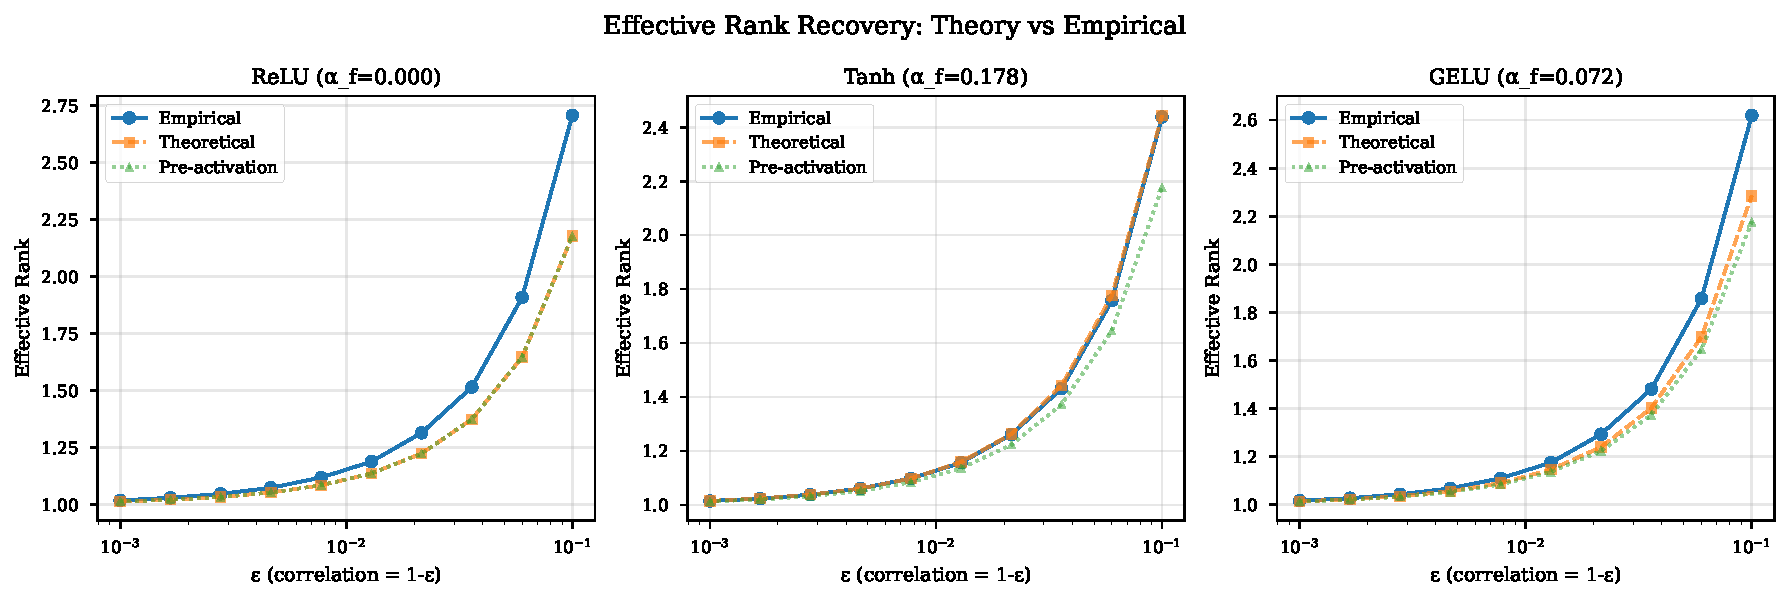
\includegraphics[width=0.9\linewidth]{validation_effective_rank_formula.pdf}
    \caption{Validation of the theoretical effective rank recovery formula. For three activation functions (ReLU with $\alpha_f=0.5000$, Tanh with $\alpha_f=0.6667$, and GELU with $\alpha_f=0.5449$), we compare empirical effective rank (circles) against theoretical predictions (dashed squares) across different correlation levels $\epsilon$. The x-axis shows $\epsilon$ where input correlation is $1-\epsilon$. The dotted line shows pre-activation effective rank. The close agreement between theory and experiment validates our formula $\tilde{r}(C_f) \approx \tilde{r}(C)(1 + \alpha_f \epsilon \ln(n/\epsilon))$, demonstrating that the rank recovery strength $\alpha_f = \frac{\mathbb{E}[f'(z)^2]}{\mathbb{E}[f(z)^2]} - 1$ accurately predicts the effective rank improvement.}
    \label{fig:validation_effective_rank_formula}
\end{figure}

The experiment uses 100-dimensional Gaussian data with varying correlation levels. The empirical results closely match our theoretical predictions across all tested activation functions and correlation levels, confirming the validity of our rank recovery coefficient $\alpha_f$ and its role in quantifying activation effectiveness.

\paragraph{Validation 3: Emergence of Frozen States from Extreme Modulation.}
Figure~\ref{fig:validation_frozen_states} directly validates Corollary~\ref{cor:max_alpha_frozen_formal}, showing that attempts to maximize rank recovery strength through extreme modulation paradoxically lead to frozen units.

\begin{figure}[ht!]
    \centering
    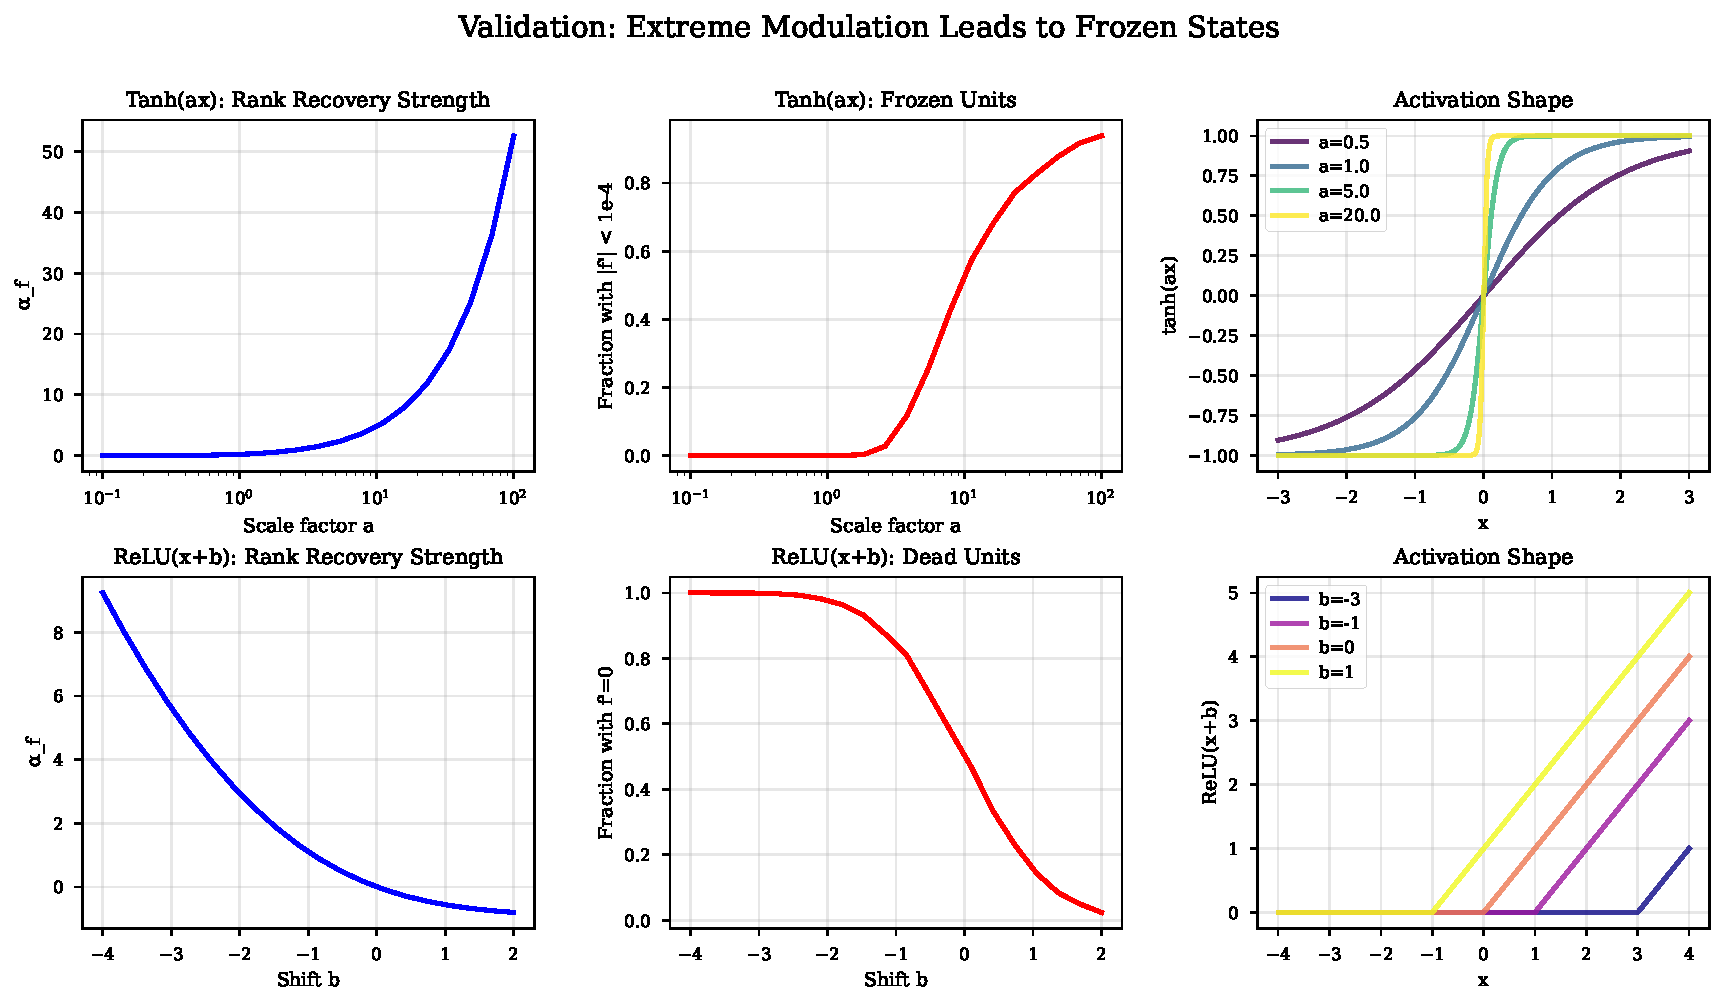
\includegraphics[width=0.9\linewidth]{validation_frozen_states.pdf}
    \caption{Validation that extreme modulation leads to frozen states. \textbf{Top row:} Analysis of Tanh(ax) with increasing scale $a$. Left: Rank recovery strength $\alpha_f$ increases with $a$. Middle: Fraction of frozen units (with $|f'| < 10^{-4}$) approaches 1 as $a$ increases. Right: Activation shapes showing saturation for large $a$. \textbf{Bottom row:} Analysis of ReLU(x+b) with negative shift $b$. Left: $\alpha_f$ varies with shift. Middle: Fraction of dead units increases as $b$ becomes more negative. Right: Activation shapes showing increasing dead zones. These results confirm Corollary~\ref{cor:max_alpha_frozen_formal}: maximizing rank recovery strength drives activations into regimes with zero gradients almost everywhere.}
    \label{fig:validation_frozen_states}
\end{figure}

For Tanh, as the scaling factor $a$ increases, we observe both increasing $\alpha_f$ and an increasing fraction of frozen units, ultimately approaching the sign function where gradients vanish almost everywhere. For ReLU with negative bias, extreme shifts create predominantly dead units. This validates our theoretical insight about the fundamental trade-off between rank recovery and gradient flow.

\paragraph{Validation 4: Comprehensive 2D Analysis of Modulation Effects.}
Figure~\ref{fig:validation_modulation_2d_comprehensive} provides a comprehensive view of how different activation functions respond to simultaneous scaling and shifting, revealing the complex landscape of frozen states and rank recovery.

\begin{figure}[ht!]
    \centering
    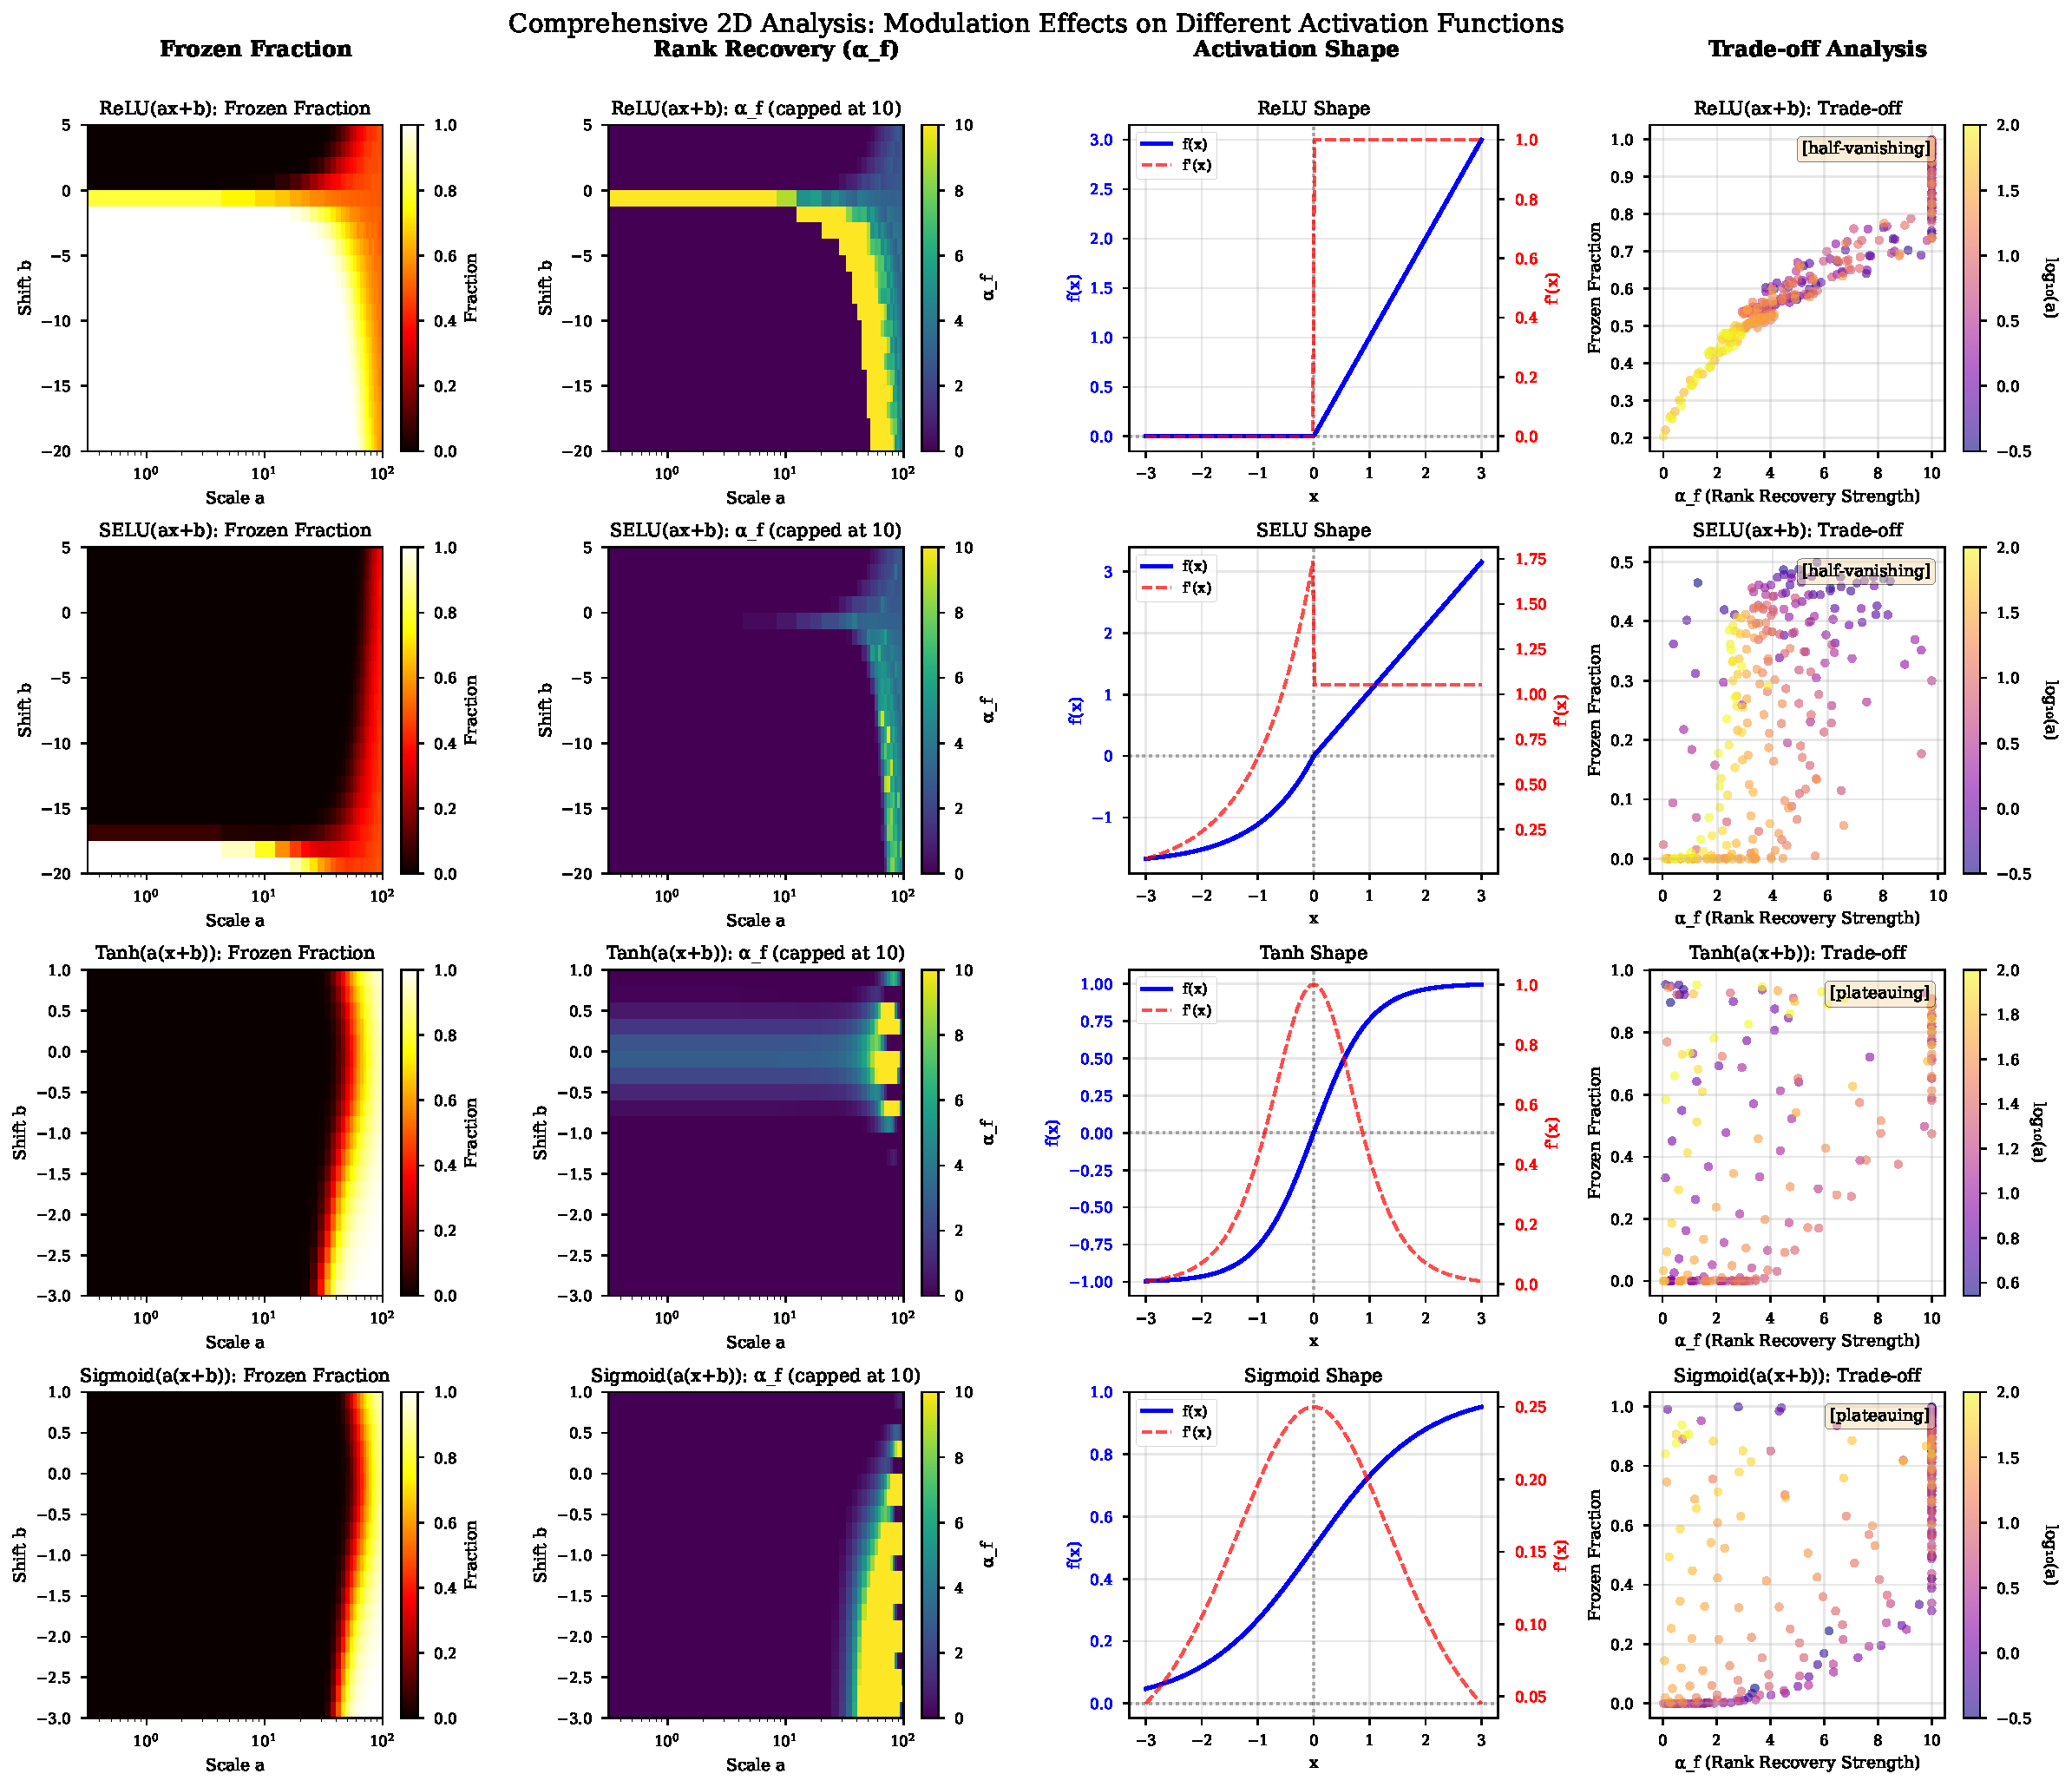
\includegraphics[width=\linewidth]{validation_modulation_2d_comprehensive.pdf}
    \caption{Comprehensive 2D analysis of modulation effects on activation functions. Each row shows a different activation function (ReLU, SELU, Tanh, Sigmoid) with their modulation scheme. \textbf{Column 1:} Heatmaps of frozen fraction as a function of scale $a$ and shift $b$. Red regions indicate parameter combinations leading to frozen/dead units. \textbf{Column 2:} Heatmaps of rank recovery strength $\alpha_f$ (capped at 10 for visualization). \textbf{Column 3:} Activation function shapes showing both $f(x)$ (blue) and $f'(x)$ (red dashed). \textbf{Column 4:} Trade-off analysis showing the correlation between $\alpha_f$ and frozen fraction, with colors indicating $\log_{10}(a)$. The analysis reveals that half-vanishing activations (ReLU, SELU) and plateauing activations (Tanh, Sigmoid) exhibit different pathways to frozen states, but all show the fundamental tension between rank recovery and maintaining gradient flow discussed in Section~\ref{sec:emergence_lop}.}
    \label{fig:validation_modulation_2d_comprehensive}
\end{figure}

This comprehensive analysis reveals several key insights:
\begin{itemize}
    \item \textbf{Half-vanishing activations} (ReLU, SELU): Large negative shifts create extensive dead zones where gradients are exactly zero, while positive shifts reduce non-linearity by making the activation nearly affine.
    \item \textbf{Plateauing activations} (Tanh, Sigmoid): Large scales cause saturation with near-zero gradients at the extremes, while the specific shift determines the balance between positive and negative saturation.
    \item \textbf{Universal trade-off}: All activation types exhibit regions in parameter space where high rank recovery ($\alpha_f$) coincides with high fractions of frozen units, empirically confirming our theoretical predictions.
\end{itemize}

These numerical validations collectively demonstrate that our theoretical framework accurately captures the fundamental mechanisms underlying both the benefits (rank recovery) and risks (frozen states) of non-linear activations in neural networks. The results underscore the delicate balance required in neural network design and training to maintain both representational diversity and gradient flow, key factors in preventing Loss of Plasticity.


\subsection{LoP manifolds: Formal Statement and Proof}
\label{app:cloning_manifold_details}

This section provides the formal definitions, statement, and proof for the LoP manifold proposition. Since the frozen manifold argument is self explanatory, we will only prove the cloning manifold result that is more non-trivial. 


First, let us introduce our neural network network formalization. 
A feed-forward neural network is defined by a directed acyclic graph $G=(V,E, w)$, where $V$ is the set of nodes (neurons), $E$ is the set of directed edges (connections), $E$ representations the structure of the computational graph of the network, and  $w:\E \to \R,$ is the weight parameters of the network, which will be denoted $w(u,v)$ for each edge $(u,v)\in E$. Furthermore, $V_{\text{in}} \subset V$ are the input nodes, and $V_{\text{out}} \subset V$ are the output nodes. The post-activation $h(v)$ of a node $v \in V$ is computed as:
\[
h(v)=
\begin{cases}
x_v, & \text{if } v\in V_{\text{in}},\\
f_v \Big(\underbrace{\Sigma_{u\in \text{in}(v)}w_{u,v}\,h(u)}_{\text{pre-activation }z(v):=}\Big), &\text{otherwise}.
\end{cases}
\]
Here, $x_v$ is the input value for input node $v$, $f_v$ is the activation function associated with node $v$, $\mathrm{in}(v)$ is the set of nodes with edges towards $v.$ The network output is the vector of activations $h(V_{\text{out}})$. 

With the formal pass formally define, we can now define our backward passes.  Given a loss function $\Loss(h(V_{\text{out}}),y)$ comparing the network output $h(V_{\text{out}})$ to a target $y$, the back-propagation algorithm computes gradients via error signals $\delta(v)$. The error signal is defined recursively:
\[
\delta(v)=
\begin{cases}
\partial\Loss(h(V_{\text{out}}),y)/\partial h(V_{\text{out}}), & \text{for output nodes },\\[4pt]
\displaystyle\sum_{u\in\mathrm{out}(v)}\delta(u)\,w(v,u)\,f'_u(z(u)), &v\notin V_{\text{out}},
\end{cases}
\]
where $\mathrm{out}(v)$ is the set of nodes receiving input from $v$, and $f'_u$ is the derivative of the activation function $f_u$. The gradient of the loss with respect to a weight $w(u,v)$ is then given by $\partial\Loss/\partial w(u,v)=\delta(v)\,f'_v(z(v))\,h(u)$.



% (For example, detailed proof for Proposition~\ref{prop:hard_rank_increase_main}, Proposition~\ref{prop:frozen_duplicate_lop}, and the original Proposition 4.1 on rank recovery via Hermite polynomials would go here).

% Proof for Prop 3.1 (Non-linearity Increases Hard Rank) -> now prop:hard_rank_increase_main
% Proof for Prop 4.1 (Existence of LoP Manifolds) -> now prop:frozen_duplicate_lop
% Original Prop 4.1 (Rank Recovery with Non-linearity Hermite Expansion)
% Original Prop B.2 (Cloned-Unit Plasticity Loss more detailed)
% Lemma on maximal rank increase -> frozen units (Corollary~\ref{cor:max_alpha_frozen_formal})
% ...

\paragraph{Network partition and base network definitions.}
Let $G = (V, E, w)$ be the main network. A partitioning refers to a partitioning of nodes defined as:
$$
\cup_{i=1}^k S_i = V, \qquad S_j\cap S_i=\emptyset\text{ for all } i\neq j.
$$

Given the partitioning, we  define the base network $\BaseG = (\BaseV, \BaseE, \BaseW)$ where each partition is a node, the edges are union of edges between two corresponding partitions, and weights are the sum total sum of edges divided by the number of rows:
$$
\BaseV:=\{S_i: i\in[k]\}
\qquad 
\BaseE = \left\{(S_i,S_j): S_i\times S_j\cap E\neq \emptyset \right\}
\qquad
\BaseW_{ij} = \frac{1}{|S_i|}\sum_{u\in S_,v\in S_j} w_{uv}.
$$

We can view the base graph as a ``meta'' graph, whose nodes are set of nodes, and its edges correspond to set of edges of the main graph. While the node and edge definitions are standard, the weight definition is slightly deviating from one might expect from standard quotient graph definitions, where the weights are total sum without averaging. The reason for this is more specific to our construction and is there to ensure similarity of the cloned and base networks forward and backward passes. 


\paragraph{Definitions of Weight Manifolds}
Given a network partitioning $S_1,\dots , S_k$, and the corresponding base graph $\BaseG = (\BaseV, \BaseE, \BaseW)$, here are the manifold definitions:

\begin{itemize}
    \item  The Row-wise Equitable (RE) manifold consists of all cloned weight matrices $w$ such that for every connection $(i,j) \in \BaseE$ in the base network, each block $w[S_i, S_j]$ all row-sums are equal:
    $$
\ManifoldRE = \left\{ w\in \R^{|E|} \;\middle|\; \forall (i,j) \in \BaseE, \text{ and } \forall r,r' \in S_i, \text{ it holds } \sum_{u \in S_j}  w_{r u} = \sum_{u \in S_j}  w_{r' r} \right\}
$$

The Column-wise Equitable (CE) manifold, consists of all cloned weight matrices $w$ such that for partitioned block $w[S_i, S_j]$ , all column sums are equal:
$$
\ManifoldCE = \left\{ w\in \R^{|E|} \;\middle|\; \forall (i,j) \in \BaseE, \text{ and } \forall c,c' \in S_j, \text{ it holds } \sum_{u \in S_i}  w_{u c} = \sum_{u \in S_i}  w_{u c'} \right\}
$$

\item The Block-wise Constant (BC) manifold consists of all cloned weight matrices $w$ such that for every block $w[S_i, S_j],$ all its elements are equal:
$$
\ManifoldBC = \left\{ w\in \R^{|E|} \;\middle|\; \forall (i,j) \in \BaseE, \text{ and } \forall u,u' \in S_i, \forall v,v' \in S_j, \text{ it holds }  w_{uv} = w_{u'v'} \right\}
$$
\item Finally, we can define the family of all duplicate manifolds, that are affine sub-spaces of the parameters. For any matrix with row and column equitability, $w\in \ManifoldRE\cap\ManifoldCE,$ they shift the block constant manifold $\ManifoldD.$ Formally:
$$
\mathbb{M}_D = \left\{ \ManifoldD(w) \;\middle|\; w\in \ManifoldRE\cap\ManifoldCE \right\}, \qquad \ManifoldD(w):= \left\{w+T\;\middle|\; T\in \ManifoldBC \right\}
$$
\end{itemize}

Note that all the manifolds defined above are linear or affine sub-spaces, as their constraints are all linear. 

There are two important facts worth mentioning that will shed more light on the upcoming proposition. 

\begin{remark}
Note that the dimensionality of manifolds in the family $\mathbb{M}_D$ are given by the number of blocks in $W,$ as opposed to number of its elements. Thus, for example if the partitioning of units forms blocks of size $n,$ we would roughly expect $1/n^2$ fewer dimensions in $\mathbb{M}_D$ than in the original full parameter space. 
\end{remark}

Furthermore, the following remark clarifies why we define these networks as cloned networks. Because when we are on these manifolds, the clone network units form perfect copies of the base network units. 

\begin{remark}
    If $W \in \ManifoldRE,$ any unit in a block $v \in S_k,$ the forward activations will be identical to the corresponding base unit $h(v) = h(\tilde{v}),$ where $\tilde{v}$ is the corresponding unit in the base network to block $S_k.$ If we further assume  $W \in \ManifoldRE\cap \ManifoldCE,$ we will have a similar property for the backwards $\delta (v) = \delta (\tilde{v}).$
\end{remark}

Let us re-state the proposition on cloning to make this section more self-contained. 

\begin{proposition}[Cloned-Unit Manifold (Re-stated)]
\label{prop:cloned_manifold_restated}
Let $G=(V,E,W),$ denote a network that is partitioned with $S_1,\dots, S_k. $ 
For any input and label $(x,y)$:

    \begin{enumerate}
        \item If $W \in \ManifoldRE$, then all units in the same cluster $u,v \in S_k$  have identical forward activations $h(u) = h(v).$
        % Original:  w&\in \text{RE}(W) \implies h(u)=h(v) = h(k) && \forall u,v\in S_k,\forall k \\
        \item If $W \in \ManifoldRE \cap \ManifoldCE$, then all units in the same cluster $u,v \in S_k$  have identical backward activations $\delta(u) = \delta(v).$ Furthermore, the gradients $\partial \Loss/\partial W$ will have a block-wise constant structure, such that gradients between any two units in two blocks will be equal, i.e., for any $u,u'\in S_i$ and $v,v'\in S_j,$ we have $\partial \Loss/\partial W_{uv} = \partial \Loss/\partial W_{u'v'}.$  
        % Original:  w&\in \text{RE}(W)\cap \text{CE}(W) \implies \nabla_{ w_{uv}}\Loss = \nabla_{w_{i,j}}\Loss && \forall u\in S_i, v\in S_j\forall i,j
        \item If the model weights at initialization or any point in training touch, if they lie on a manifold from the family  $W\in \ManifoldD$ where $\ManifoldD \in \mathbb{M}_D,$ given any arbitrary batches of input label pairs used to obtain subsequent model parameters $W(t), $, any subsequent training parameter trajectory constrained to the same manifold:
    \begin{align*}
    W(0)\in \ManifoldD \implies    W(t) \in \ManifoldD && \text{$\ManifoldD\in \mathbb{M}_D$, $t$ gradient steps}
    \end{align*}
\end{enumerate}

\end{proposition}

\begin{proof}[Proof of Proposition~\ref{prop:cloned_manifold_restated} (Cloned-Unit Manifold)]
The proof will be done as a series of inductions. 
First, let us assume that we have sorted the units in a topological order $v_1,\dots, v_n$ which exists because the network is a directed acyclic graph. Let us further assume that input nodes appear first in this list, and that outputs as the last edges in the list. Finally, because we assume no edges inside each block between the units, let us assume that the units in the same block are adjacent in our topological sort. Thus, for any two distinct blocks $S_i\neq S_j,$ we either have all nodes in $S_i$ before $S_j$ or vice versa, but cannot have a mix. 

\paragraph{Forward cloning.} Row-equitability assumption implies identical forward for units in the same block. The induction hypothesis is that for all $k,$ any preceding unit $p \le k,$ that belongs same partition  $ u_p, u_k \in S_i ,$  will have identical forward $h(u_p) = h(u_k). $ Because cloning does not apply to input units, meaning that every unit is a separate block, the hypothesis trivially holds for all input units $k=1,\dots, d$ where $d$ is input dimension. Now, let us prove the induction step, assuming step $k.$ Let $p\le k$ correspond to a unit in the same block $u_p,u_k  \in S_i. $ Now, consider all the units that have incoming edges to these two units, which necessarily must appear before $p$. Let's consider all such units within the same block $S_j.$ Because these units appear before $k,$ the induction hypothesis tells us that they have identical forward. Thus, the total contribution from these units to pre-activations $z(u_p)$ and $z(u_k)$ will be proportional to sum of edge weights from units in $S_j$. Because of our construction of the ordering, all the units in $S_j$ that feed into $S_i$ must occur before them. 
Now, the row-equal assumption implies that the sum of weights from all these units to $u_p $ and $u_k$ must be equal weight sum. Thus, we have proven that pre-activation contribution from units in  $S_j$ will be identical for $u_p$ and $u_k$. Because we chose $S_j$ arbitrarily and it could have been any block, we have proven that pre-activation these units must be identical $z(u_p)=z(u_k)$. Since they also have identical activation function, they will have identical outputs $h(u_p)=h(u_k)$. This completes the induction hypothesis for forward pass cloning. 

\paragraph{‌Backward cloning.} We want to prove that column and row-equitability assumption implies identical backward for units in the same block. The  proof strategy will be highly similar to the forward cloning case, with the key difference that our induction will be backward in our ordering, starting from latest output units and then moving in backward in the list. The induction hypothesis for step $k$ is that, for al $q > k$, if they are in the same block $u_k,u_q\in S_i$, they will have identical backwards $\delta(u_k)=\delta(u_q).$ Because output units are not themselves cloned, the induction step holds trivially for the last output nodes. Now let us prove the induction hypothesis for $k$ assuming that it holds for all higher steps. Now, for some arbitrary block $S_j$ that units in $S_i$ feed into, consider all outgoing connections from $u_k,u_q$ to the units in this block. Because of our construction of the ordering, all the units in $S_j$ that $S_i$ feeds into must occur after $S_j.$ Thus, by induction hypothesis, all these units must have identical backwards. Furthermore, from our column-equitability assumption we know that total edge weights from $u_k,u_q$ to these units must be identical. Thus, the summation formulas in the backward of $u_k$ and $u_q$ are similar. Finally, since $S_j$ was chosen arbitrarily, this summation is identical for all subsequent blocks, which implies the overal sum is also identical. To conclude the proof, note that because of row-equitability condition we already inherit the proof from the forward case, implying  $f'(z(u_k)) = f'(z(u_q)). $ Thus, both parts to the backward formula for $u_k,u_q$ will be identical, which proves they have identical backwards. This finishes the induction step. 

\paragraph{Gradient cloning.} This step is a straightforward consequence of the forward and backward cloning steps, and the formula that gradient of an edge from $u$ to $v$ is simply $h(u)\delta(v).$ Thus, the cloning structures in forward and backward, manifest themselves as a block structure in the gradients. 

\paragraph{Constrained training trajectory.} Here, the key induction step is over the gradient steps. For step $t,$ the induction hypothesis is that $W(t) \in \ManifoldCE\cap\ManifoldRE,$ and that $W(t)-W(0) \in \ManifoldBC. $ This trivially holds for initial step $t=0.$ Let us prove the induction step $t+1$ assuming that it holds for $t.$ Suppose gradient at this step $\Delta W(t)$ is defined over the loss arbitrary number of samples $\{(x_i,y_i)\}.$ Because of the induction hypothesis $W(t) \in \ManifoldCE\cap\ManifoldRE,$ our earlier results imply that the gradients for each sample $\partial \Loss_i / \partial W(t),$ will have a block-wise constant structure $\partial \Loss_i / \partial W(t) \in \ManifoldBC. $ Thus, the sum of these gradients will also have a block-wise constant structure $\Delta W(t) := \partial \Loss_ / \partial W(t) \in \ManifoldBC. $ Because block-wise matrices are also row- and column-equitable, this implies that the new weights will inherit those $W(t+1) = W(t) + \Delta W(t) \in \ManifoldCE\cap\ManifoldRE. $  Finally, our parameter shift can be written as $W(t+1)-W(0) = \Delta W(t) + W(t)-W(0), $  where $W(t)-W(0)  $ is a block-wise constant matrix and thus $W(t+1)-W(0)$ becomes sum two block-wise constant matrices, which is itself block-wise constant $W(t+1)-W(0)\in \ManifoldBC. $ This finishes our induction step. 

\end{proof}



\section{Empirical Appendix}
\label{app:empirical_evidence_appendix}
This section provides comprehensive details of the experimental setups, additional empirical results, figures supporting claims made in the main text, and visualizations.

\subsection{Experimental Details}
\label{sec:experimental_details}

This section outlines the experimental setup, methodologies, and general procedures employed for the empirical analysis of Loss of Plasticity (LoP) in neural networks.

\subsubsection{Overview of Experimental Paradigms}
\label{subsec:experiment_paradigms}

Our investigation into LoP encompasses three primary experimental paradigms.

\textbf{Continual Learning experiments} involve training models on a sequence of temporally independent tasks where data from previously learned tasks is unavailable. Tasks are typically formulated by partitioning the output classes of standard datasets, and for any given task $t$, the model is trained exclusively on its assigned class subset $\mathcal{C}_t$. The training protocol included optional reinitialization of model output layer weights and biases are reset to zero before starting each new task to mitigate interference.

\textbf{Neural Network Cloning experiments} study the effects of neuron duplication , using a two-stage training protocol. Initially, a base model is trained on a target task to establish baseline performance. Subsequently, this base model is expanded by a specified factor (always fixed to two), using the cloning procedures detailed later.  The expanded (cloned) model is then trained. To compare the base and cloned model, we also keep training the base model at the same time during this second phase. The results presented here are all CIFAR10 dataset, and we used 20 epochs to train the base model and 500 epochs to train the cloned model. This cycle can be iterated. Functional equivalence post-cloning is verified by ensuring the cloned model produces activations identical to its base, assessed via $R^2$ scores between corresponding layer activations. $R^2$ scores, computdd for each layer, measure if the mean of cloned units can explain the variance of all units in that block. 

\textbf{Bit Flipping experiments} simulate a slowly-changing regression problem to evaluate network adaptability to gradually drifting input distributions. A target network with Linear Threshold Units (LTUs), where an LTU computes $\text{LTU}(s) = \mathbf{1}_{s \ge 0}$ (i.e., 1 if $s \ge 0$, 0 otherwise), implements $h_i = \text{LTU}(w_i^T x - \theta_i)$ and $y = w_{\text{out}}^T h + b_{\text{out}}$, where $\theta_i = (m \cdot \beta) - S_i$ and $S_i = \sum_{j: w_{ij} < 0} 1 - 0.5 \cdot w_{i,m+1}$. Input consists of $m$ bits plus a bias bit; $f$ of these bits are ``flipping bits'' changing every $T$ time steps (one randomly selected flipping bit is inverted), while the remaining $m-f$ bits are randomly sampled each step. A two-layer MLP with a configurable activation function is trained online to learn this target. % 

\subsubsection{Core Methodologies and Implementations}
\label{subsec:core_methodologies}

Several core methodologies underpin our experiments.


\paragraph{Cloning Implementation.}  Our cloning implementation is modular. For each architecture, we first need to decide the ``free'' parameter to expand. This is the feature dimension for MLP and ViT, and channels for CNN and ResNet. After creating a base and expanded model, our cloning implementation proceeds in a modular fashion. The key implementation idea that allowed this modular design is the principle that the cloning profile of inputs and outputs of different modules must be consistent. For example if inputs A and B to a module are assumed to be cloned, and if these are output by a different modules, that module must ensure this cloning. We can think of this as a matching cloning profile between connected modules. With this design in mind, for linear layers, weights and biases are replicated according to input/output expansion factors; weights connected to cloned input neurons are scaled (e.g., by $1/\alpha_{\text{in}}$ for an input duplication factor of $\alpha_{\text{in}}$) to maintain activation magnitudes. Convolutional layers see similar expansion of input/output channels, with kernels tiled and appropriately scaled while preserving spatial dimensions. For normalization layer, if affine features are learned, their cloning will be a simple duplication for different cloned units. The same applies to modules such as patch embeddings, which require a simple duplication.  Parameterized activations (e.g., PReLU) have their parameters correspondingly duplicated or broadcast. Any other units that does not have parameters, such as softmax layer or activations without parameter, will not require any particular treatment, because it has the potential to create cloning profiles that do not match.  
To fix this, we implemented a clone-aware flattening operation in CNNs ensures duplicated channels remain adjacent after flattening to preserve structure for subsequent fully-connected layers.

\paragraph{Noisy SGD optimizer} introduces Gaussian noise $\epsilon_t \sim \mathcal{N}(0, \sigma_t^2 \|g_t\|^2 I)$ to gradients $g_t$, where the noise scale $\sigma_t = \sigma_0 \cdot \lambda^t$ decays over time $t$ from an initial value $\sigma_0$. The values of $\sigma_0$ and $\lambda$ are hyperparameters of the optimizer. Later, we show the effect of varying them on the cloned model dynamics.
 
\paragraph{Continual Backpropagation (CBP)}, implemented in \texttt{src/utils/cbp\_optimizer.py} following the Generate-and-Test framework, aims to maintain plasticity by selectively replacing low-utility neurons. Utility tracking involves measures like \emph{Contribution Utility} ($(u_{\text{contrib}}^{(t)}))_i = |h_i^{(t)}| \cdot |\bar{w}_{\text{out},i}|$) and \emph{Adaptable Contribution} ($(u_{\text{adapt}}^{(t)})_i = \frac{|h_i^{(t)} - \bar{h}_i^{(t)}| \cdot |\bar{w}_{\text{out},i}|}{|\bar{w}_{\text{in},i}|}$), where $h_i^{(t)}$ is activation, $\bar{h}_i^{(t)}$ is its running average, and $\bar{w}$ terms are mean weight magnitudes. Instantaneous utilities are smoothed using an exponential moving average ($\rho$ is decay rate, $a_i^{(t)}$ is neuron age): $u_i^{(t)} = \rho u_i^{(t-1)} + (1-\rho) \tilde{u}_i^{(t)}$, with a bias-corrected version $\hat{u}_i^{(t)} = u_i^{(t)}/(1 - \rho^{a_i^{(t)}})$. Neuron replacement occurs for eligible mature neurons ($a_i > \tau_{\text{maturity}}$) with the lowest utility (a fraction $r_{\text{replace}}$ of layer neurons $N_L$). Selected neurons are reinitialized (incoming weights via Kaiming, outgoing to zero, utility/age reset). A bias correction ($b_{\text{next}} \leftarrow b_{\text{next}} + W_{\text{out}}[:, i] \cdot \bar{h}_i$) is applied to the subsequent layer.


% \paragraph{Metrics for Analysis} (\texttt{src/utils/metrics.py}) Our metrics include the fraction of ``dead'' neurons (near-zero activations for $>\tau_{\text{dead}}$ of inputs), ``duplicate'' neurons (normalized activation patterns with Pearson correlation $>\tau_{\text{corr}}$ with another neuron), and ``saturated'' neurons (activation gradient magnitude to mean activation ratio $<\tau_{\text{sat}}$ for $>p_{\text{sat}}$ of a batch). \emph{Representation Quality Metrics} include effective rank (from Shannon entropy of normalized singular values of the activation matrix), Stable Rank ($\|H\|_F^2 / \|H\|_2^2$), and non-Gaussianity measures (Shapiro-Wilk, Kolmogorov-Smirnov, etc.). In this paper we only present the effective rank  out of the three. \emph{Cloning Quality} is assessed by $R^2$ scores between base and cloned model activations. Specifically, given $N$ units that are cloned, we use the average of these units as the predictor, and measure the explained variance across each individual units, and compare that against variance of all units in that layer to calculate the $R^2$ score. 

\paragraph{Metrics for Analysis} Our comprehensive metric suite quantifies various aspects of network behavior and plasticity loss. \emph{Single and pair feature metrics} include the fraction of ``dead'' neurons, identified when $\frac{1}{N} \sum_{i=1}^{N} \mathbf{1}[|H_{ij}| < 10^{-7}] > \tau_{\text{dead}}$ for neuron $j$ across $N$ samples, with $\tau_{\text{dead}} = 0.95$. ``Duplicate'' neurons are detected through cosine similarity patterns, with neurons $j,k$ are considered duplicates if $\tilde{H}_j^T \tilde{H}_k > \tau_{\text{corr}} = 0.95$, where  activations are normalized by feature $\tilde{H}_j = H_{\cdot,j}/\|H_{\cdot,j}\|_2$. ``Saturated'' neurons are identified when the ratio of gradient magnitude to mean activation magnitude $|G_{ij}|/\max(\mu_j, \epsilon)$ falls below $\tau_{\text{sat}} = 10^{-4}$ for more than $p_{\text{sat}} = 99\%$ of samples in a batch. \emph{Representation diversity metrics} include effective rank, computed as $\exp(-\sum_i p_i \log p_i)$ where $p_i = \sigma_i/\sum_j \sigma_j$ are normalized singular values from the activation matrix SVD; stable rank, calculated as $\|\tilde{H}\|_F^4/\text{tr}((\tilde{H}^T\tilde{H})^2)$ for mean-centered activations $\tilde{H}$;  \emph{Cloning quality} is assessed by $R^2$ scores between base and cloned model activations, computed as $R^2 = 1 - \text{Var}(\text{residuals})/\text{Var}(\text{total})$ where the predictor is the mean of $N$ cloned units and we measure explained variance across individual units relative to the total variance in that layer. This is done for both forward and backward activations across all layers, and numbers presented here are averages across all layers and both forward and backwards for the fixed batch that we are measuring the metrics. We also keep tracking all metrics for both base and cloned model after training to provide a comparison between the two. 

\subsubsection{General Setup and Procedures}
\label{subsec:general_setup}

\paragraph{Model Architectures} include Multi-Layer Perceptrons (MLPs), Convolutional Neural Networks (CNNs), ResNets, and Vision Transformers (ViTs), with configurations (depth, width, activations, normalization layer, dropout). The default configurations are as follows:
% \paragraph{Model Architectures.} We evaluate four distinct neural network architectures with standardized configurations across experiments. 
Our Multi-Layer Perceptron (MLP) consists of $5$ hidden layers with 128 units each, employing ReLU activations, batch normalization applied before activation, and $20\%$ dropout. The Convolutional Neural Network (CNN) architecture comprises 3 convolutional layers with $[64, 128, 256]$ channels respectively, using $3\times3$ kernels with stride 1 and padding 1, followed by $2\times2$ max pooling operations. The convolutional features are processed by a single fully connected layer with 512 units, with ReLU activations, batch normalization, and 10\% dropout throughout. For ResNet, we implement a ResNet-18 variant with $[2, 2, 2, 2]$ residual blocks per stage, starting with 64 base channels that double at each stage, using ReLU activations, batch normalization, and 10\% dropout. The Vision Transformer (ViT) architecture divides input images into $8\times8$ pixel patches, which are projected to $384$-dimensional embeddings and processed through $6$ transformer layers with $6$ attention heads each. The ViT employs an MLP ratio of $4.0$ (yielding hidden dimensions of 1536), GELU activations, layer normalization, and $10\%$ dropout for both general operations and attention mechanisms. All normalization layers include learnable affine parameters ($\gamma$, $\beta$), unless stated otherwise, and bias terms are enabled where applicable. Default hyperparameter configurations for each architecture can be adjusted per experiment as described in the experimental setup.

\paragraph{Datasets and Preprocessing} involve standard image classification benchmarks: MNIST ($28 \times 28$ grayscale), CIFAR-10 and CIFAR-100 ($32 \times 32$ RGB with standard augmentations like random crops and flips), and Tiny ImageNet ($64 \times 64$ RGB). Standard train/test splits are used. For all the figures and results reported here, we used tiny ImageNet dataset for continual learning experiments, while for cloning, CIFAR-10 was used.   

\paragraph{Training Configuration} involves optimizers like Adam or SGD without momentum and no weight decay with otherwise parameters in torch. The learning rates for the continual experiments where set to $0.001$ using Adam for all architectures except for Vision Transformer, which was set to $0.0001.$ For cloning experiments with dropout, we varied the learning rate on a grid $0.01, 0.001, 0.0001.$

\paragraph{Experimental Control} is maintained through comprehensive random seeding, which controls the randomness across all relevant libraries (Python, NumPy, PyTorch) and CuDNN deterministic mode.  We used 5 seeds for all experiments to calculate confidence intervals. Experiments utilize GPUs when available, falling back to CPUs otherwise. Metrics are typically computed at fixed epoch intervals (e.g., every 5 epochs), often on consistent fixed data batches for reproducibility. Computationally intensive metrics like SVD may use subsampling of the features or samples to make them less expensive. 

\paragraph{Computational Resources.}
For the continual learning and cloning experiments, our experimental grid consisted of approximately 2,000 individual runs (counting each random seed separately). These experiments were executed on a cluster of NVIDIA A100 GPUs, utilizing a heterogeneous mix of 40GB and 80GB memory variants. The total computational cost for these experiments was approximately 10,000 GPU-hours.
The bit flipping experiments and additional theory validation experiments were conducted on a more diverse set of hardware, utilizing lower-end computational nodes equipped with NVIDIA RTX 3090, V100, and RTX 2080 GPUs. This heterogeneous setup was sufficient for these less computationally intensive experiments, and the overall compute amounted to under 100 GPU-hours on these nodes.
The theoretical validation figures and numerical simulations presented in the theory appendix (Section~\ref{app:numerical_validations_activations}) were generated on a MacBook using CPU computation only.


% For \textbf{Logging, Reproducibility, and Statistics}, experiments are logged using Weights \& Biases, capturing metrics, hyperparameters, model specifications, and environment details. A Hydra-based system manages configurations. Each run generates a unique output directory with configuration snapshots, training history, and code versioning information. Key experiments are repeated with multiple random seeds (typically 3-5 or more). Results are reported as mean $\pm$ standard error/deviation, and statistical tests or effect sizes are considered where appropriate.

\paragraph{Figures details.} 
Unless stated otherwise, all our figures report standard deviations over $5$ experiment randomization, by the use of a different seed. Additionally, to reduce the number of points in the plot, in Figures 
\ref{fig:emergence_lop_symptoms_cl},\ref{fig:norm-rank-nG},\ref{fig:norm-rank},\ref{fig:CBP-scale-dup},\ref{fig:CBP-scale-rank} we plot the average over time windows of $1000$ steps. 

\subsection{Additional Figures and Empirical Substantiation}
This subsection includes placeholder figures for concepts discussed in the main text, for which specific existing figures were not available or suitable for direct inclusion in the main body.


\begin{figure}[!ht]
    \centering
    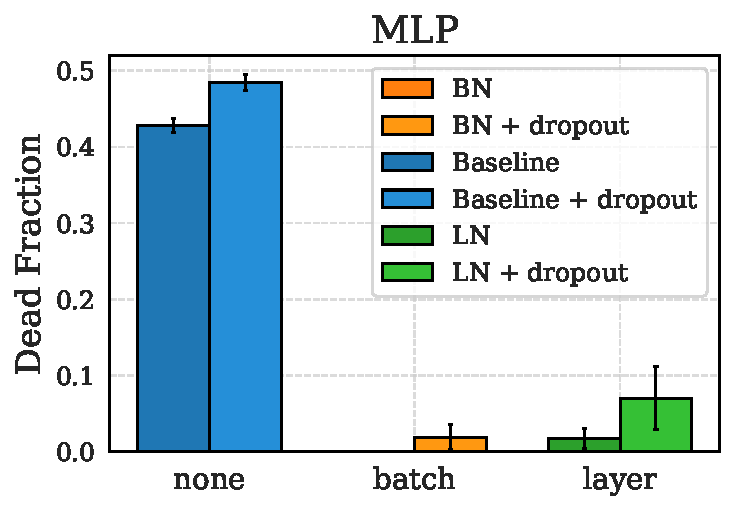
\includegraphics[width=0.2\linewidth]{paper/images/act__dead_fraction_normalizations_barplot.pdf}
    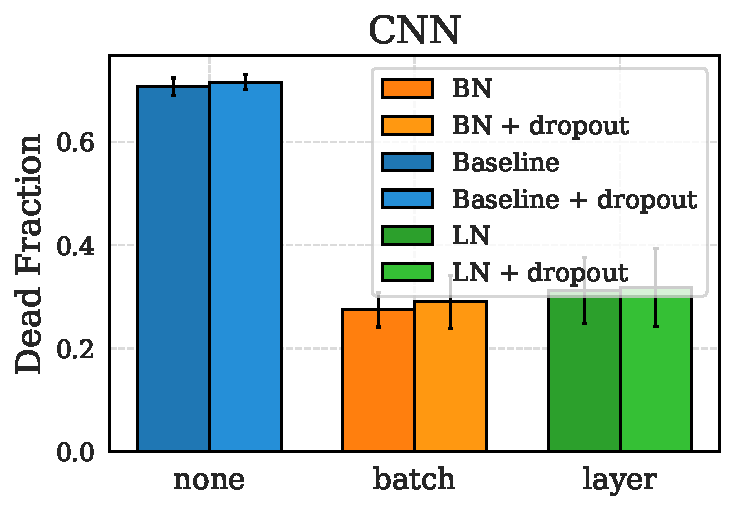
\includegraphics[width=0.2\linewidth]{paper/images/cnn_act__dead_fraction_normalizations_barplot.pdf}
    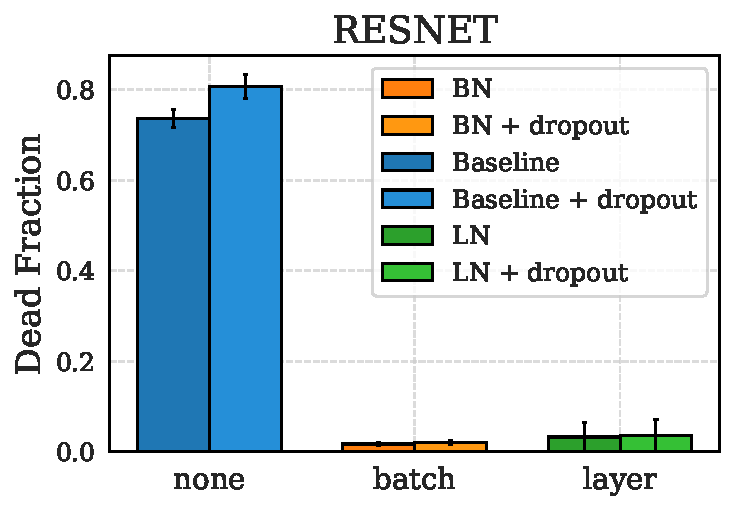
\includegraphics[width=0.2\linewidth]{paper/images/resnet_block_dead_fraction_normalizations_barplot.pdf}
    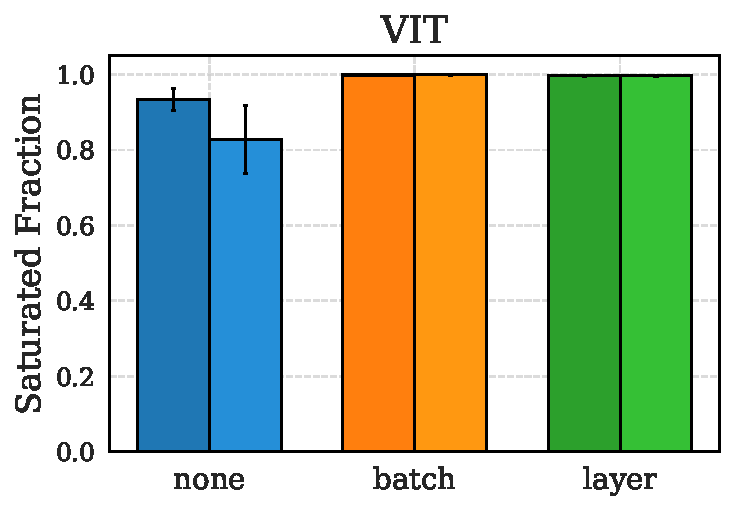
\includegraphics[width=0.2\linewidth]{paper/images/vit_block_saturated_frac_normalizations_barplot.pdf} \\
    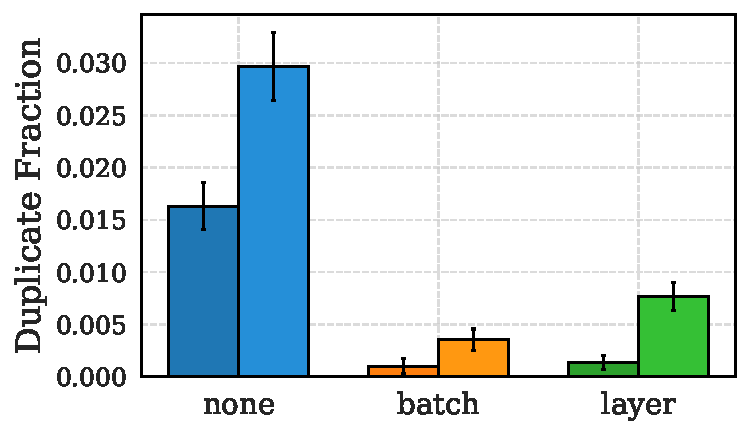
\includegraphics[width=0.2\linewidth]{paper/images/act__dup_fraction_normalizations_barplot.pdf}
    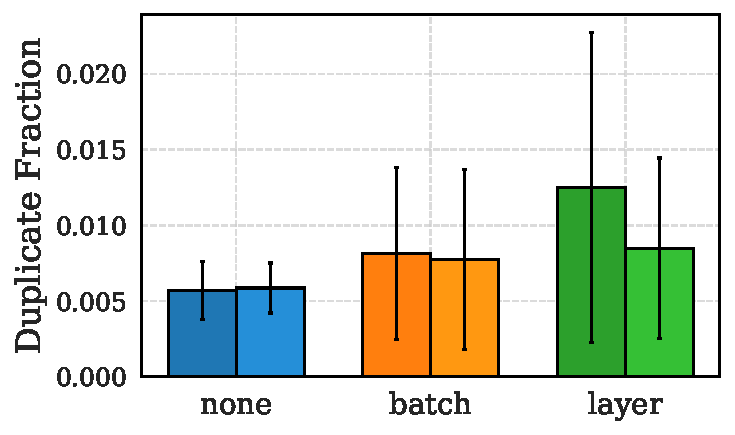
\includegraphics[width=0.2\linewidth]{paper/images/cnn_act__dup_fraction_normalizations_barplot.pdf}
    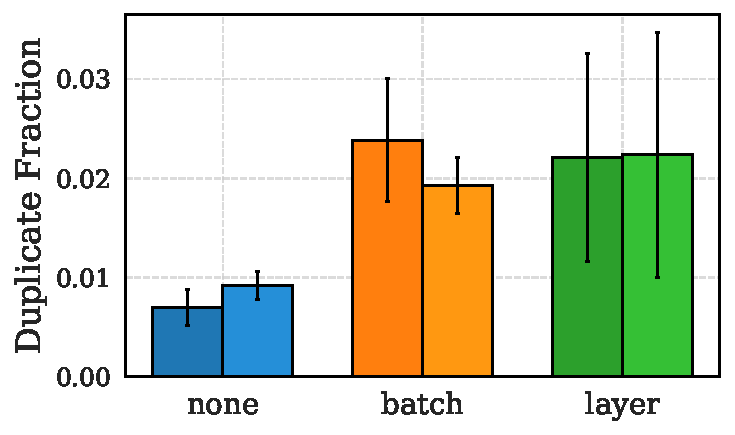
\includegraphics[width=0.2\linewidth]{paper/images/resnet_block_dup_fraction_normalizations_barplot.pdf}
    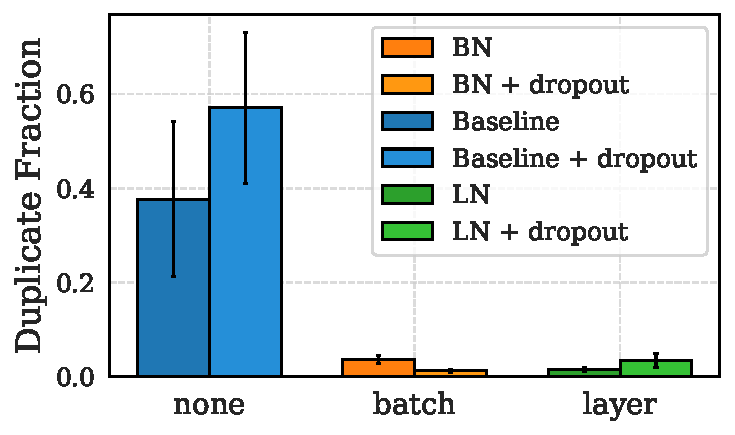
\includegraphics[width=0.2\linewidth]{paper/images/vit_block_dup_fraction_normalizations_barplot.pdf} \\
    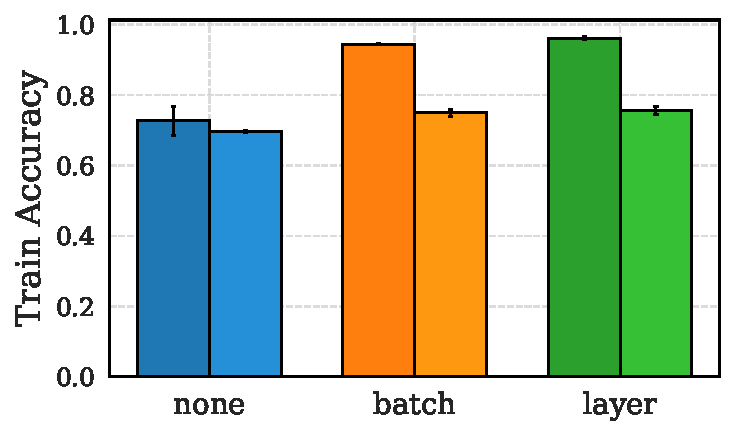
\includegraphics[width=0.2\linewidth]{paper/images/act__train_acc_p_normalizations_barplot.pdf}
    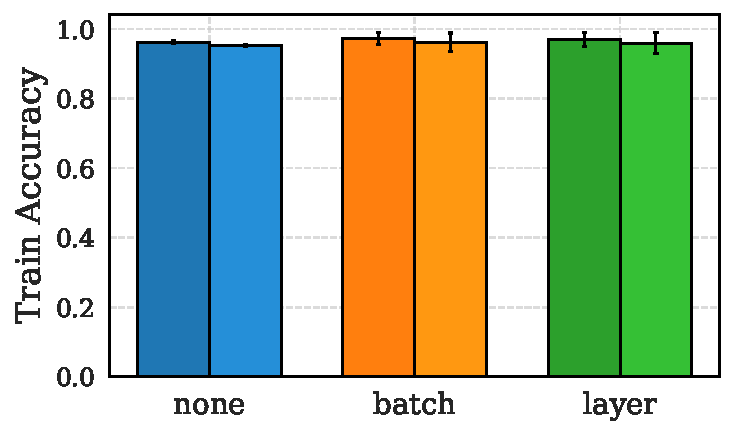
\includegraphics[width=0.2\linewidth]{paper/images/cnn_act__train_acc_p_normalizations_barplot.pdf}
    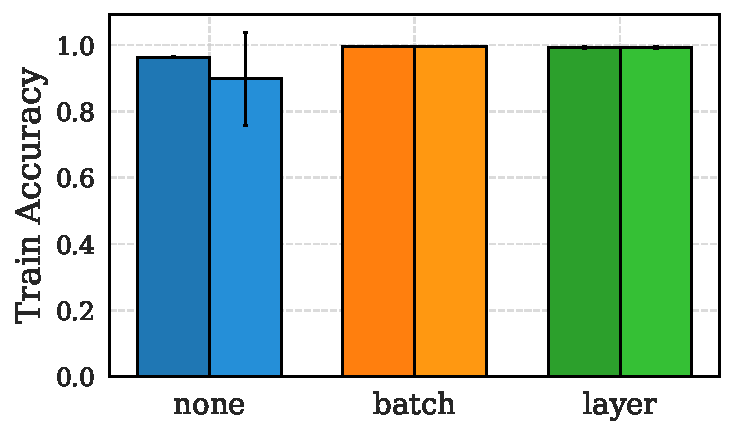
\includegraphics[width=0.2\linewidth]{paper/images/resnet_block_train_acc_p_normalizations_barplot.pdf}
    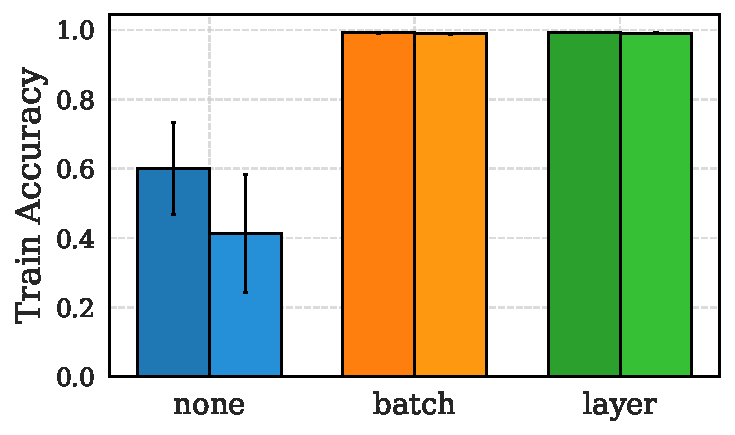
\includegraphics[width=0.2\linewidth]{paper/images/vit_block_train_acc_p_normalizations_barplot.pdf}
    \caption{Normalization reduces the number of dead/saturated units (top row) and duplicated units (middle row), and its impact on training accuracy (bottom row) across different architectures. The training accuracy displayed is calculated as the average online accuracy over the entire training length. These results highlight the role of normalization in mitigating LoP symptoms.}
    \label{fig:normalizations-recovering}
\end{figure}

\begin{figure}[!ht]
    \centering
    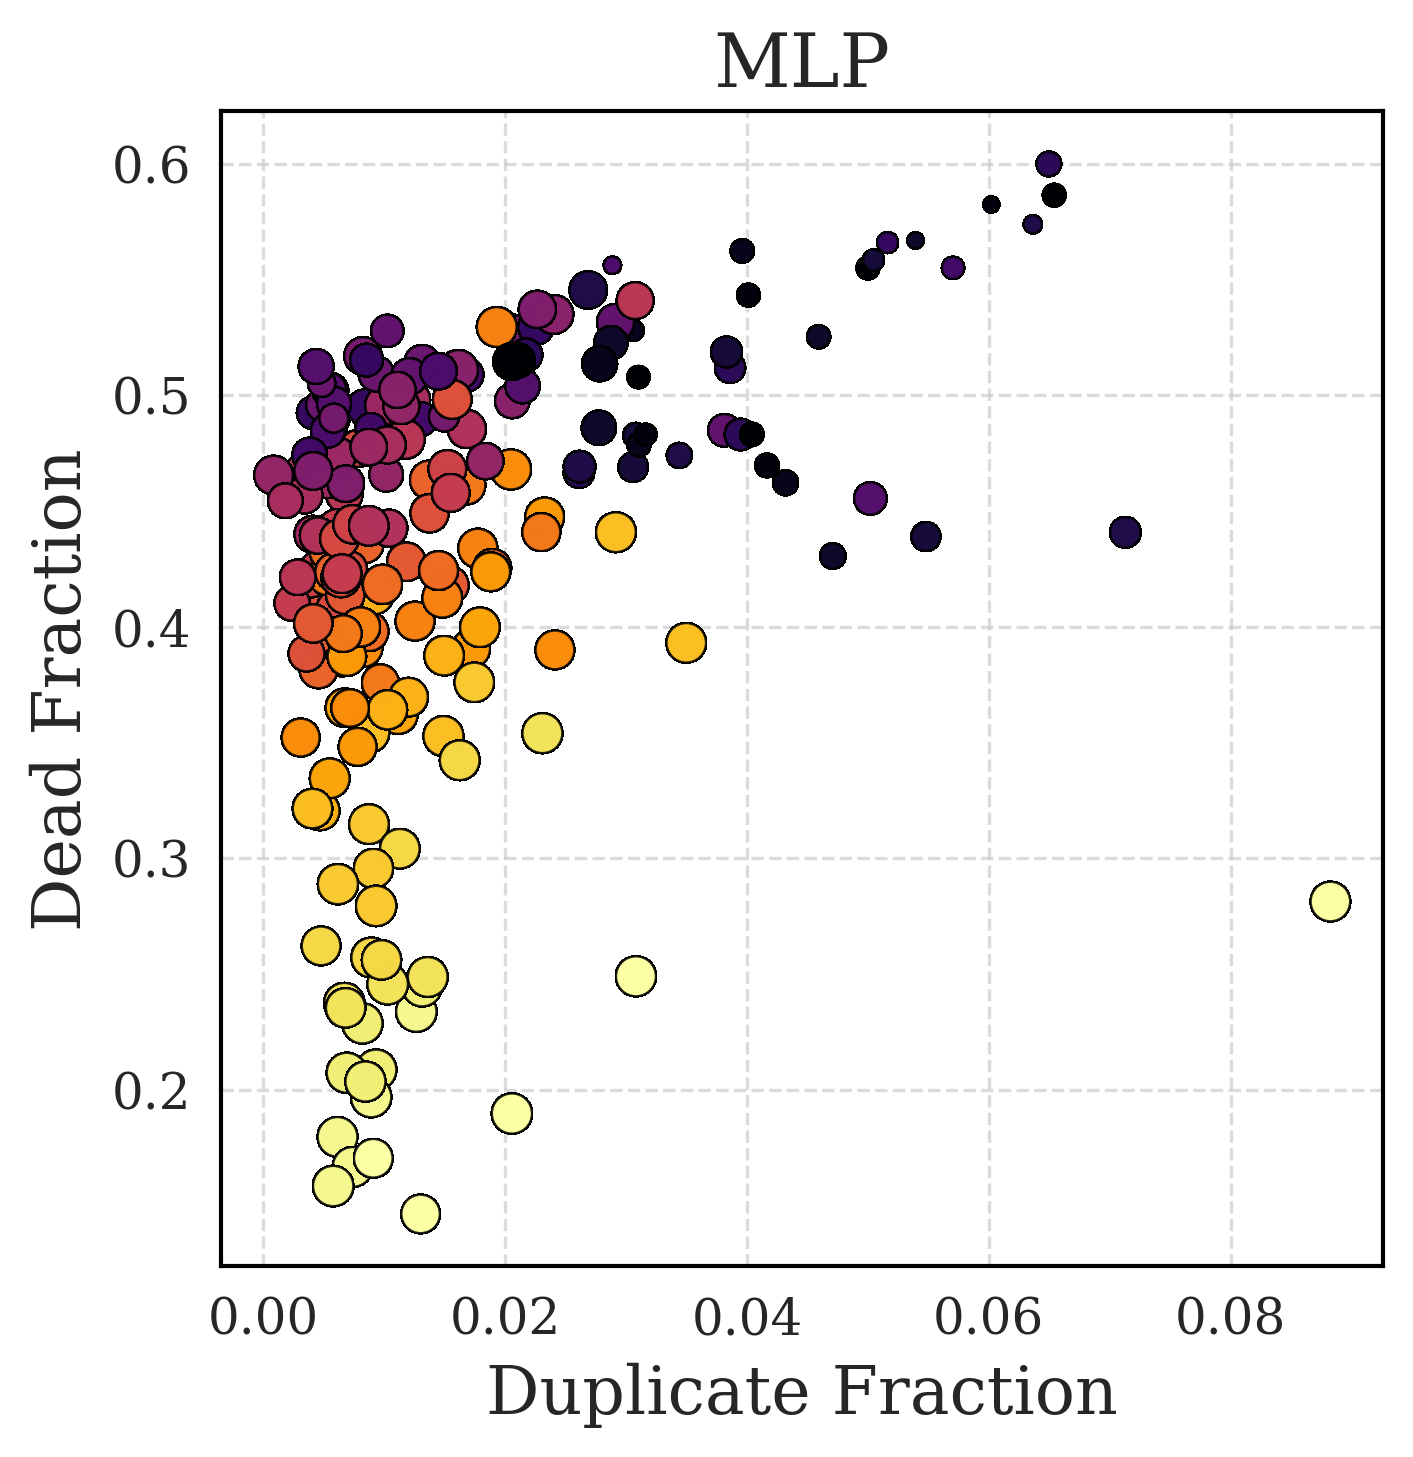
\includegraphics[width=0.23\linewidth]{paper/images/mlp_dupdeadacc_plot.png}
    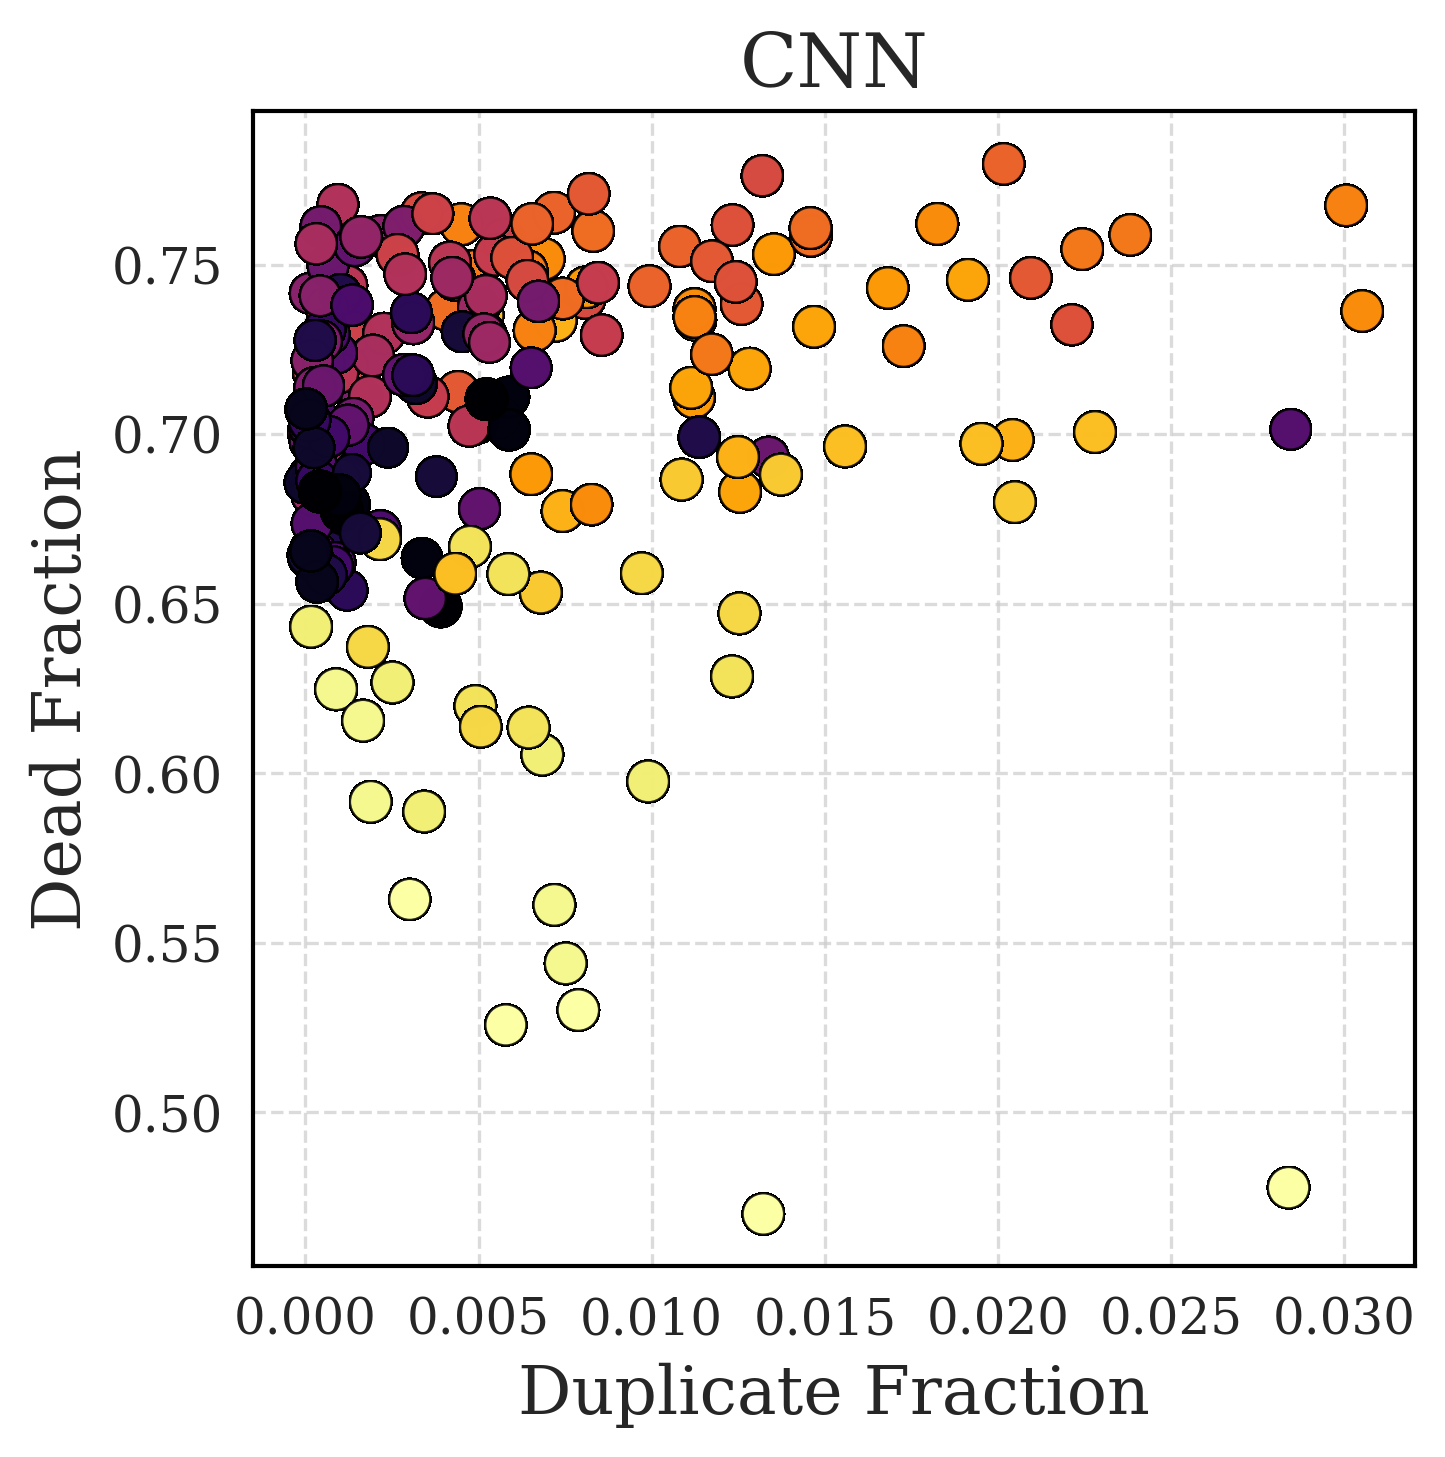
\includegraphics[width=0.23\linewidth]{paper/images/cnn_dupdeadacc_plot.png}
    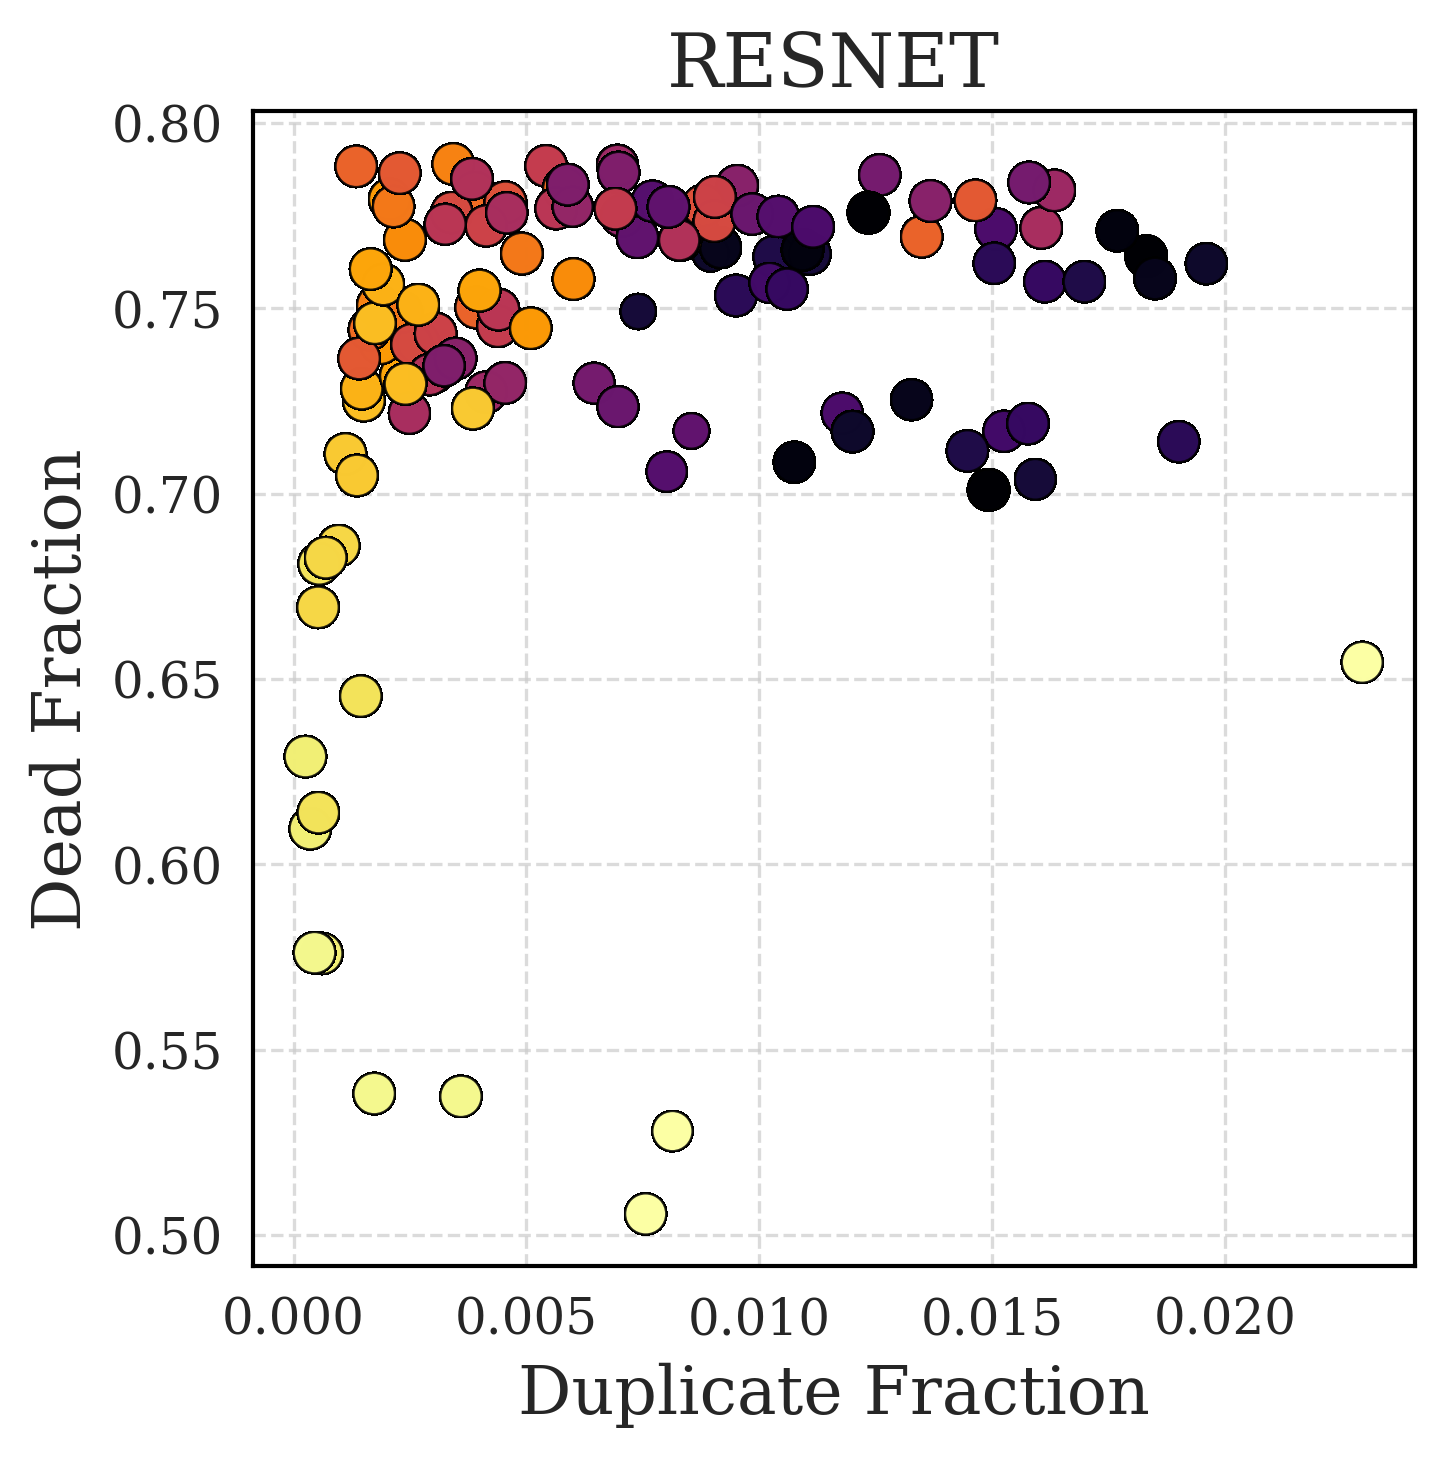
\includegraphics[width=0.23\linewidth]{paper/images/resnet_dupdeadacc_plot.png}
    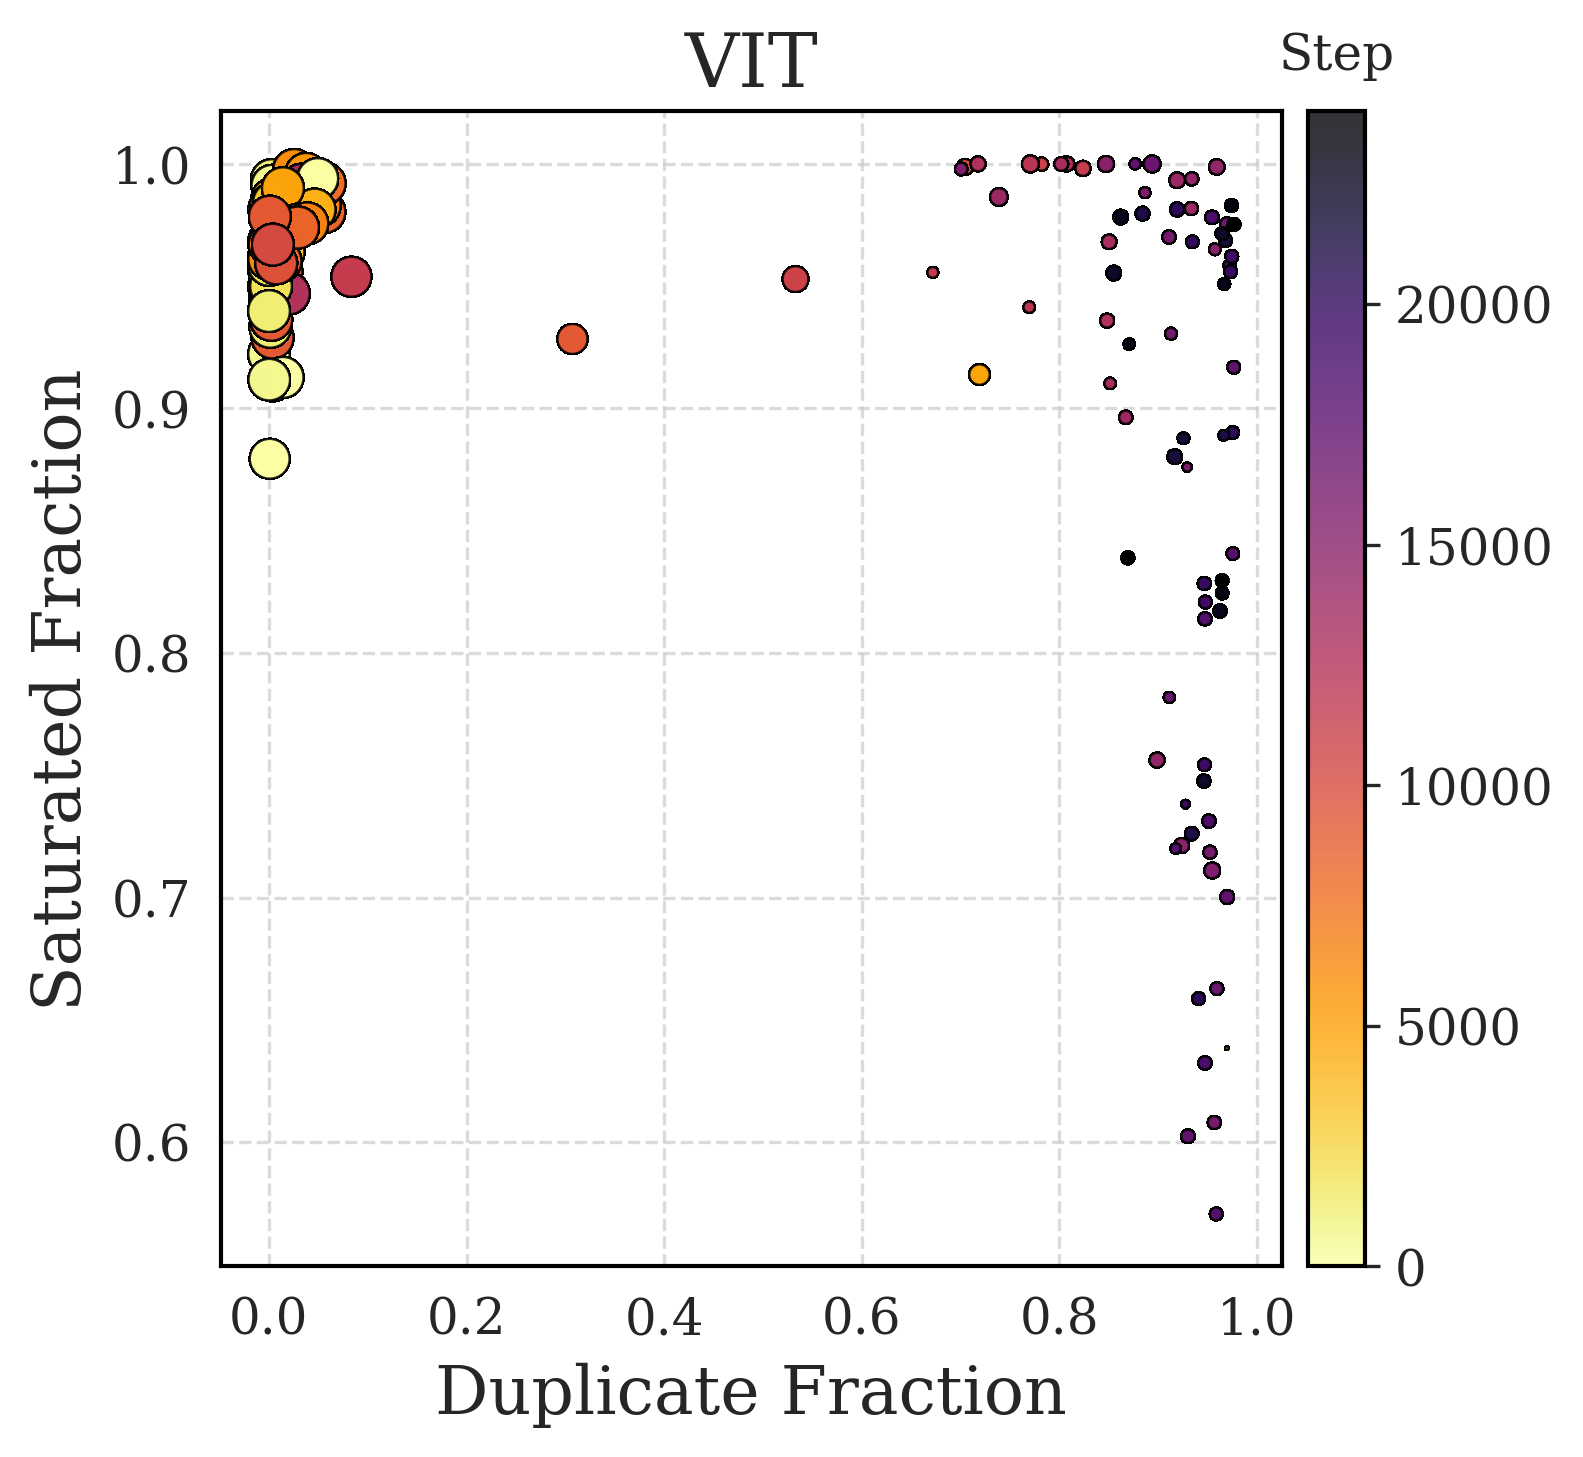
\includegraphics[width=0.25\linewidth]{paper/images/vit_dupdeadacc_plot.png}
    \caption{Evolution of duplicate/dead unit fractions and training accuracy. The colors correspond to training steps (lighter is earlier) and the points size to the Training Accuracy (bigger is higher). This figure illustrates the correlation between the increase in LoP symptoms (duplicate/dead units) and training dynamics.}
    \label{fig:dupfrac-LoP-dead-dup}
\end{figure}

\begin{figure}[!ht]
    \centering
    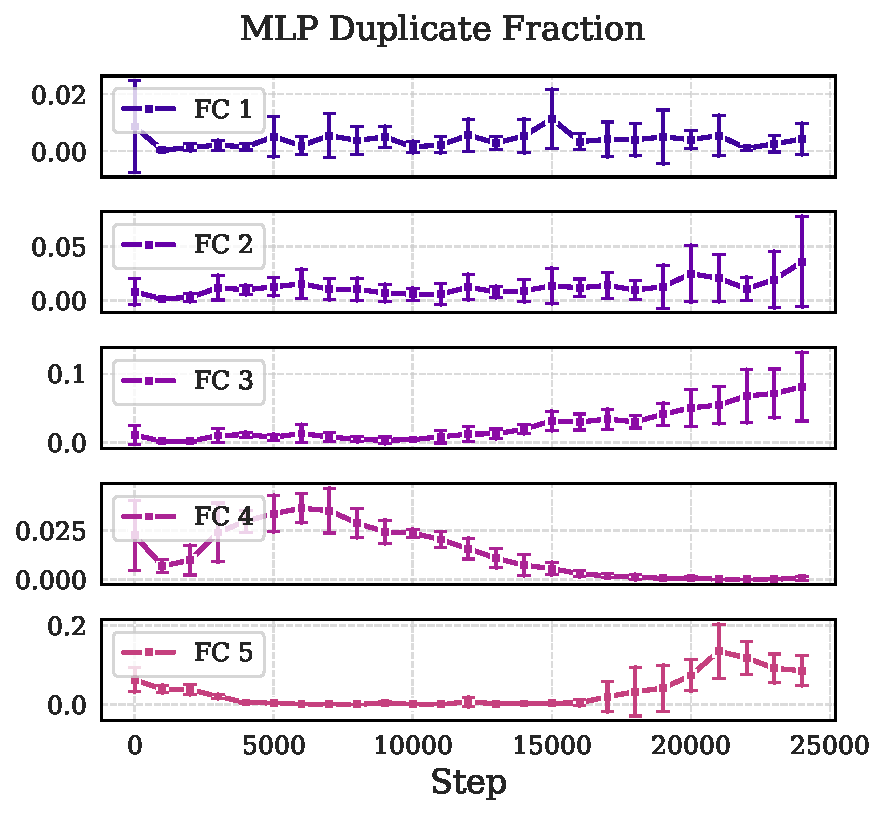
\includegraphics[width=0.24\linewidth]{paper/images/mlp_act__dup_fraction_layerwise.pdf}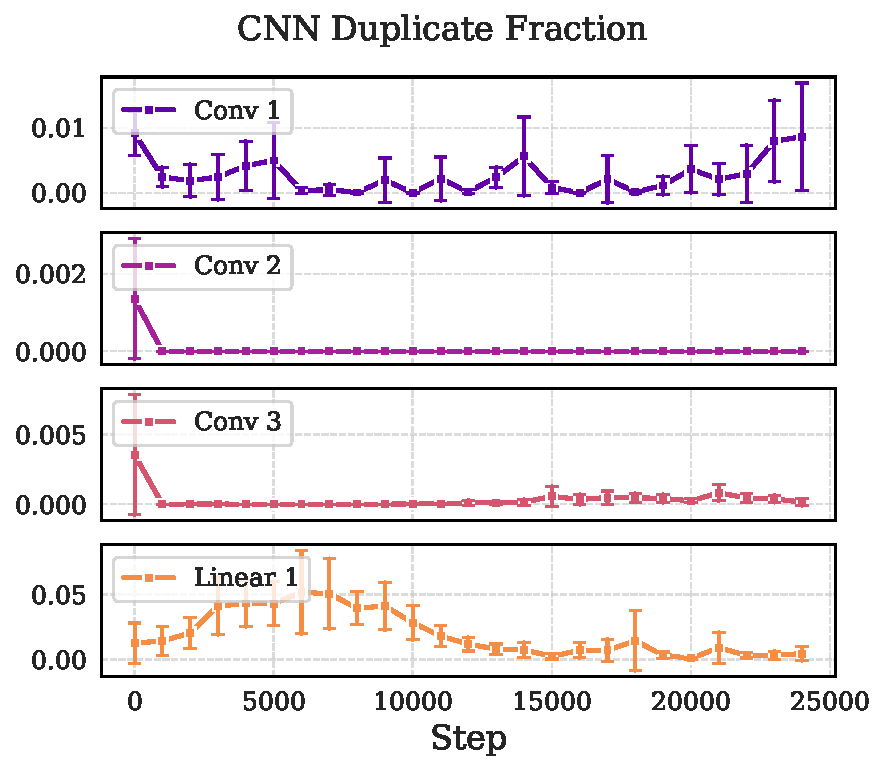
\includegraphics[width=0.24\linewidth]{paper/images/cnn_act__dup_fraction_layerwise.pdf}
    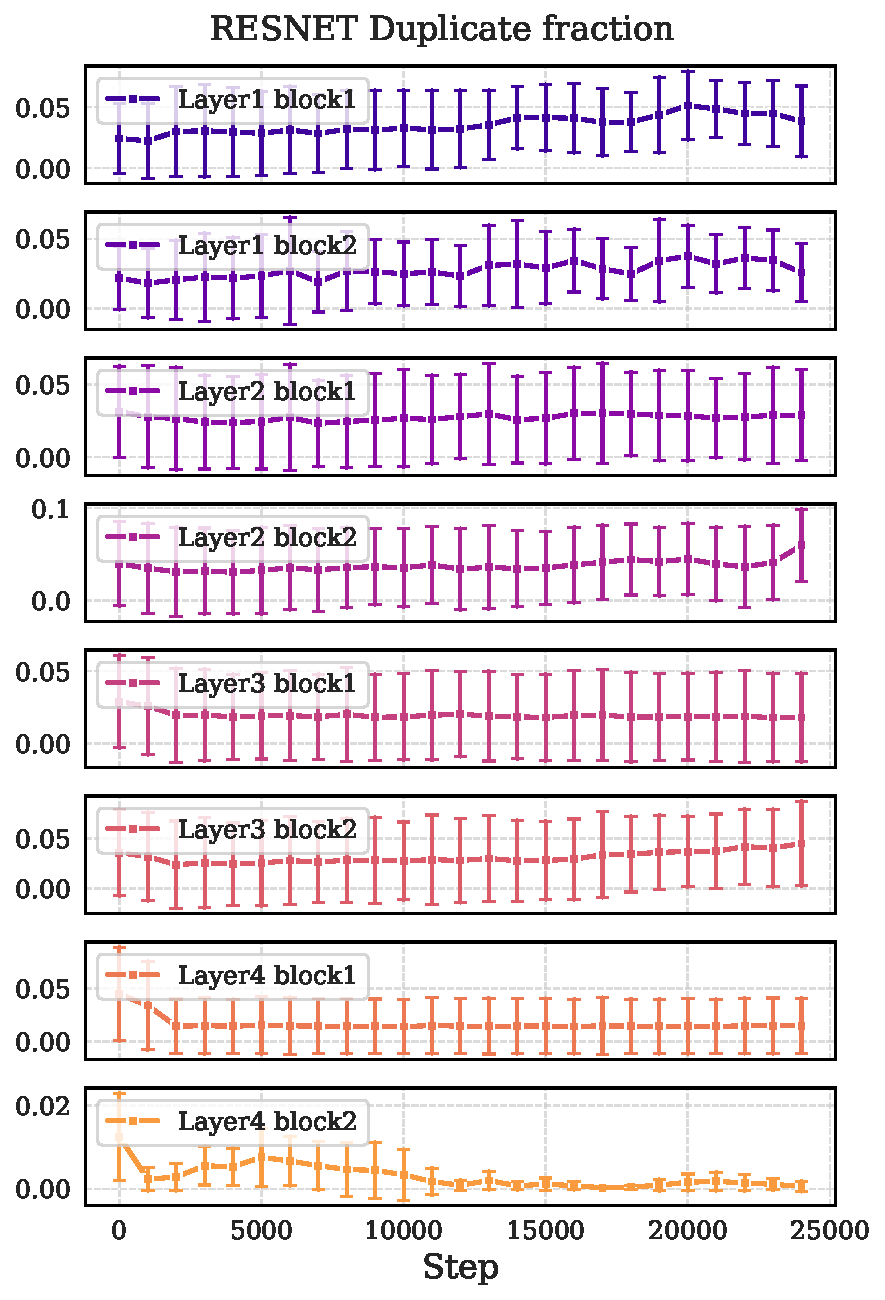
\includegraphics[width=0.24\linewidth]{paper/images/resnet_block_dup_fraction_layerwise.pdf}
    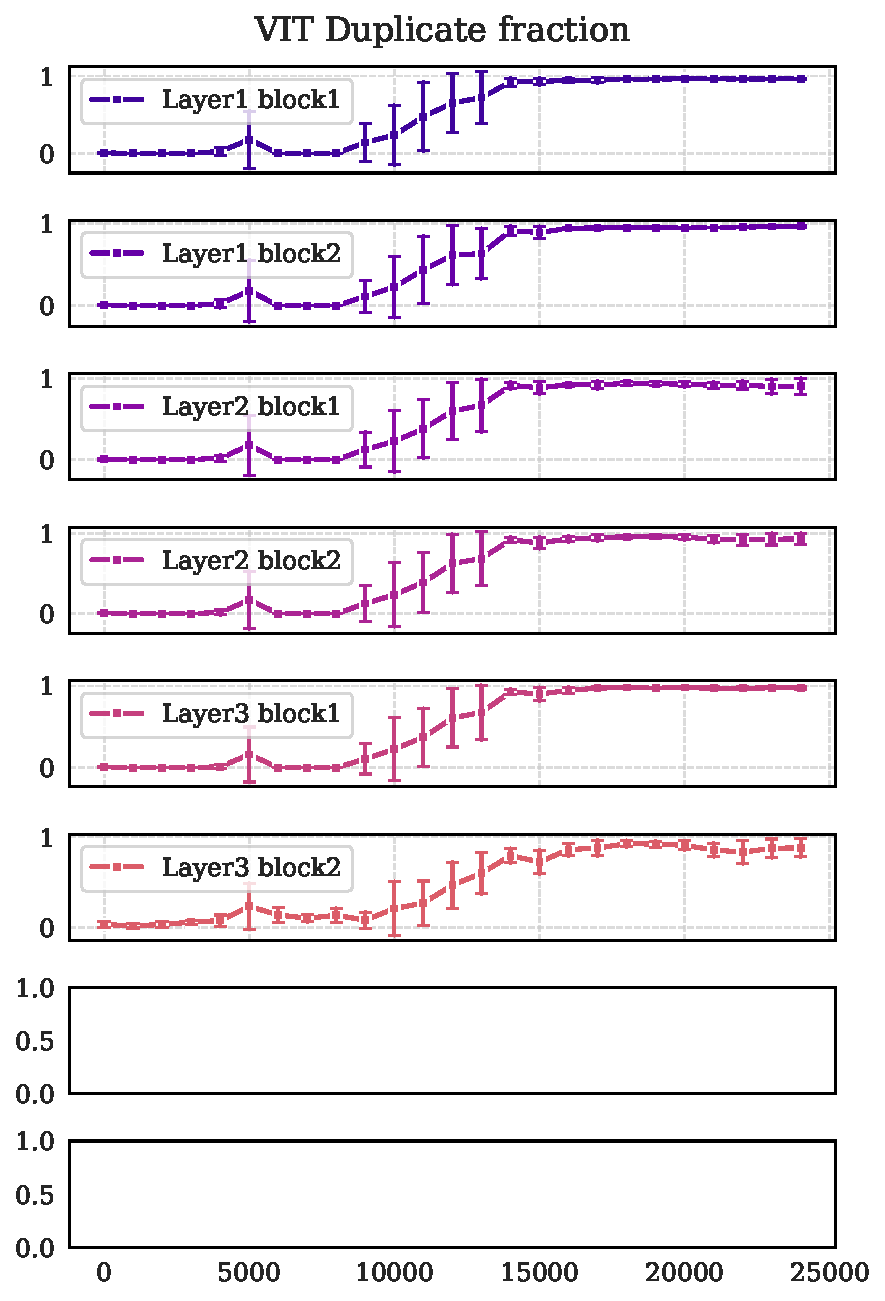
\includegraphics[width=0.24\linewidth]{paper/images/vit_block_dup_fraction_layerwise.pdf}
    \caption{Emergence of duplicate units layer-wise during training without normalization and no dropout. This figure shows the increasing fraction of duplicate units as training progresses, a symptom of LoP. }
    \label{fig:dupfrac-LoP-layerwise}
\end{figure}

\begin{figure}[!ht]
    \centering
    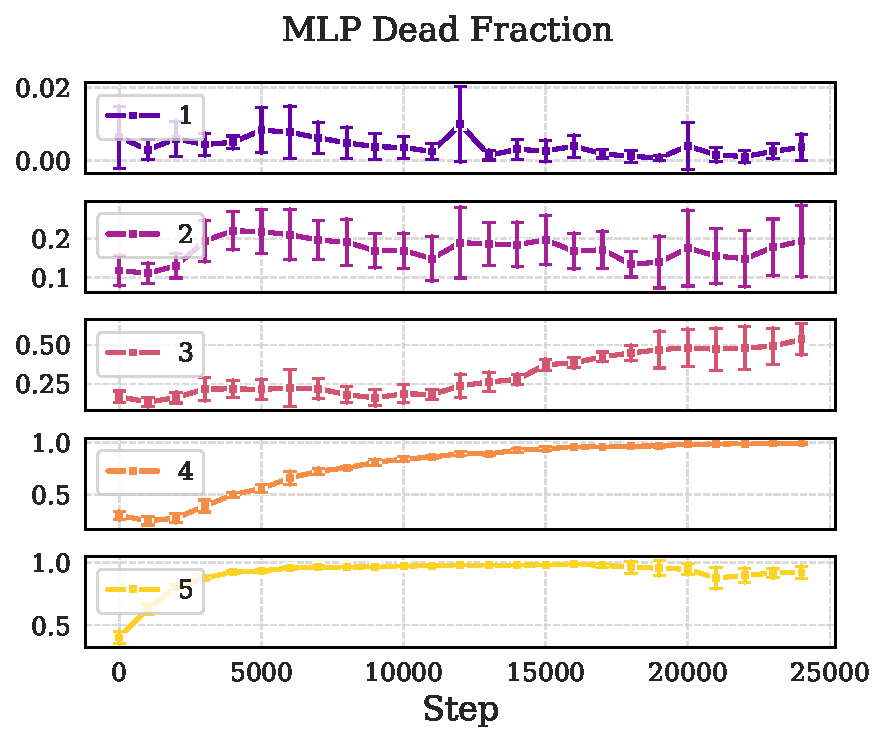
\includegraphics[width=0.24\linewidth]{paper/images/mlp_act__dead_fraction_layerwise.pdf}
    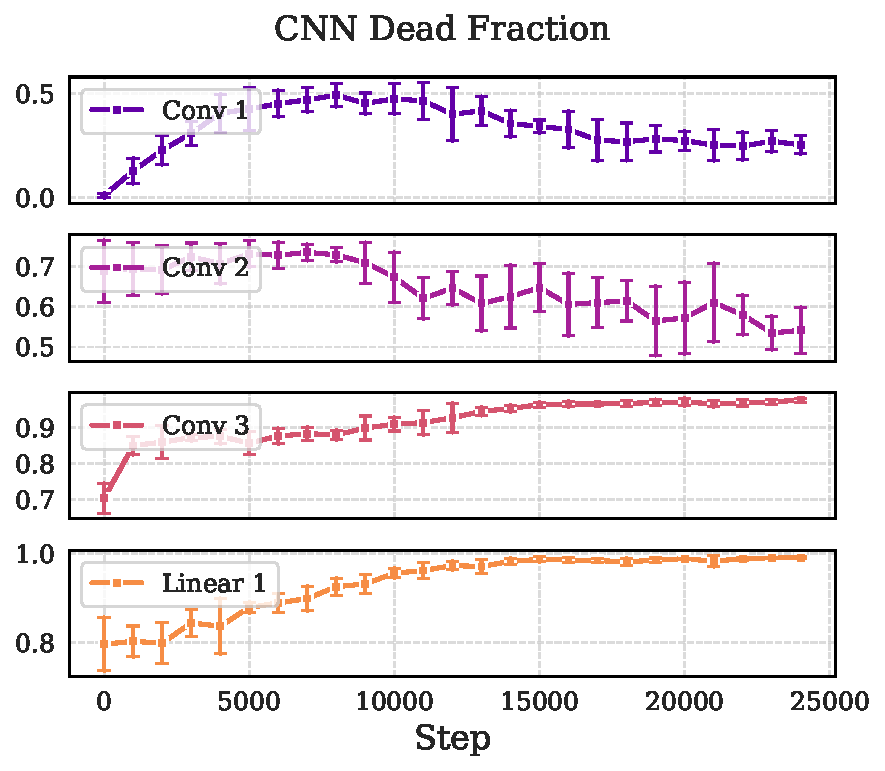
\includegraphics[width=0.24\linewidth]{paper/images/cnn_act__dead_fraction_layerwise.pdf}
    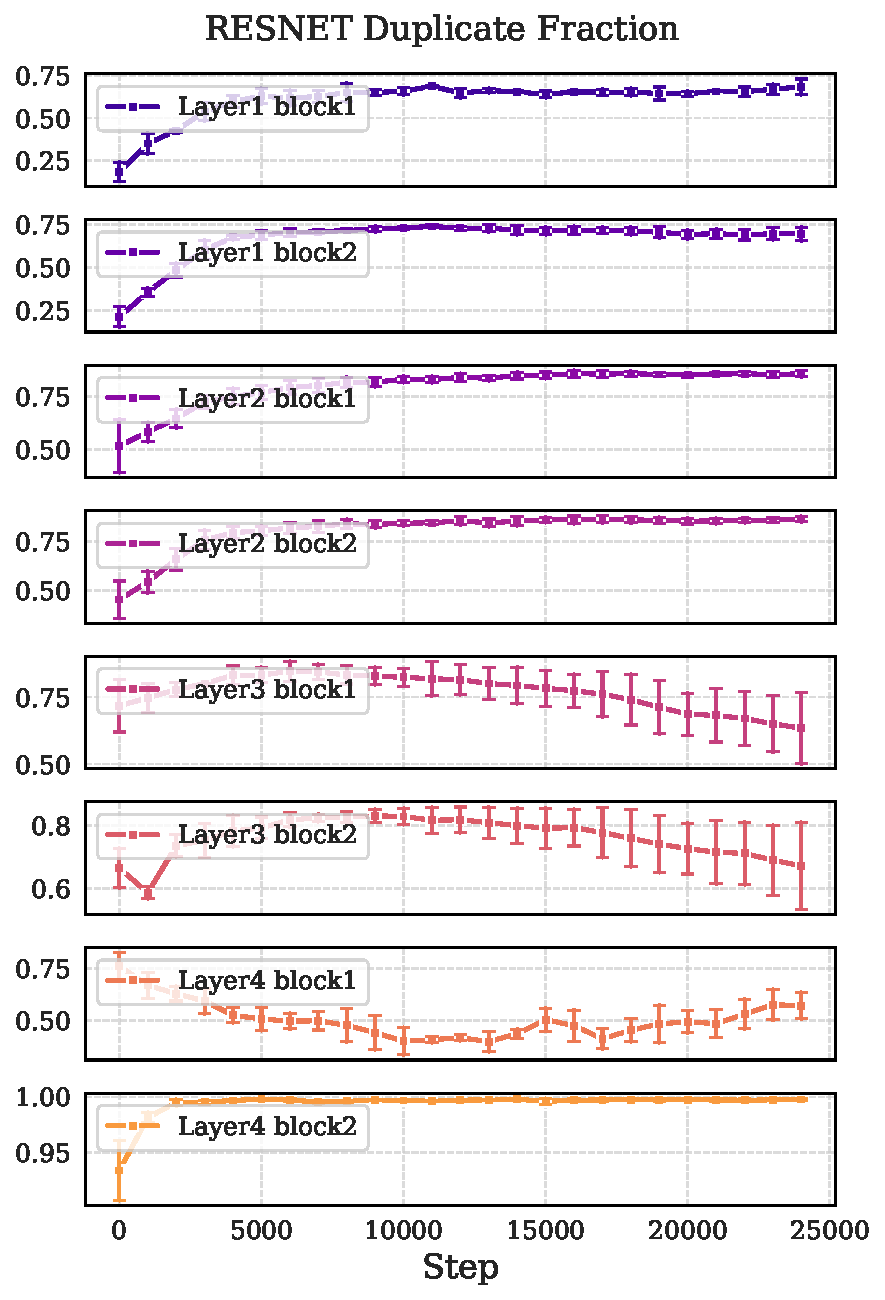
\includegraphics[width=0.24\linewidth]{paper/images/resnet_block_dead_fraction_layerwise.pdf}
    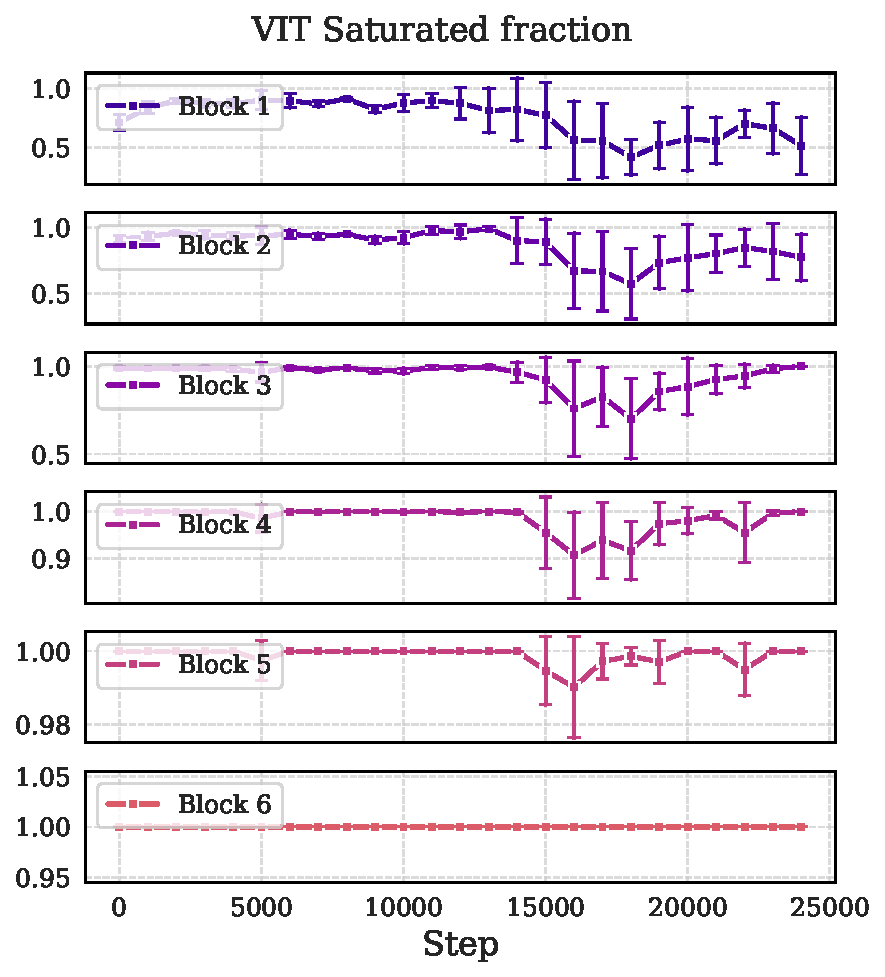
\includegraphics[width=0.24\linewidth]{paper/images/vit_block_saturated_frac_layerwise.pdf}
    \caption{Emergence of dead or saturated units layer-wise during training without normalization and no dropout. This figure shows the increasing fraction of dead units as training progresses, a symptom of LoP.}
    \label{fig:dupfrac-LoP}
\end{figure}

\begin{figure}
    \centering
    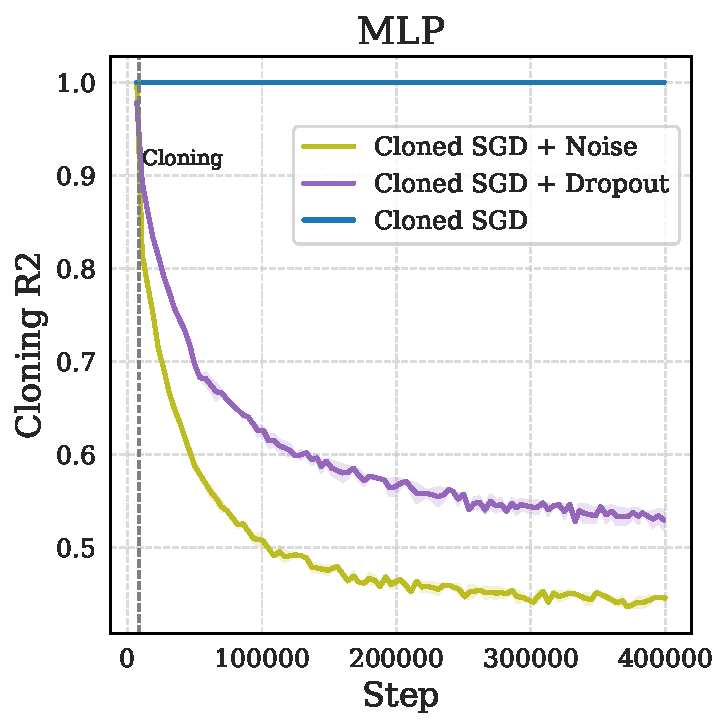
\includegraphics[width=0.3\linewidth]{paper/images/mlp_cloning_r2_plot.pdf}
    \includegraphics[width=0.3\linewidth]{paper/images/mlp_cloning_losses_plot.pdf}
    \includegraphics[width=0.3\linewidth]{paper/images/mlp_cloning_rank_plot.pdf}
    
    \includegraphics[width=0.3\linewidth]{paper/images/cnn_cloning_r2_plot.pdf}
    \includegraphics[width=0.3\linewidth]{paper/images/cnn_cloning_losses_plot.pdf}
    \includegraphics[width=0.3\linewidth]{paper/images/cnn_cloning_rank_plot.pdf}
    
    \includegraphics[width=0.3\linewidth]{paper/images/resnet_cloning_r2_plot.pdf}
    \includegraphics[width=0.3\linewidth]{paper/images/resnet_cloning_losses_plot.pdf}
    \includegraphics[width=0.3\linewidth]{paper/images/resnet_cloning_rank_plot.pdf}

    
    \includegraphics[width=0.3\linewidth]{paper/images/vit_cloning_r2_plot.pdf}
    \includegraphics[width=0.3\linewidth]{paper/images/vit_cloning_losses_plot.pdf}
    \includegraphics[width=0.3\linewidth]{paper/images/vit_cloning_rank_plot.pdf}
    
    \caption{Cloning experiments across architectures. Configurations details: SGD with LR=0.01, Noisy SGD with $\sigma = 0.01$ and $\lambda = 0.999$, and Dropout with probability $0.1$. Normalization used: Batch Norm for all architectures, except ViTs, where we use Layer Norm.}
    \label{fig:enter-label}
\end{figure}


\begin{figure}
    \centering
    \includegraphics[width=0.3\linewidth]{paper/images/mlp_noises_cloning_losses_plot_sigma_lambda_0.9.pdf}
    \includegraphics[width=0.3\linewidth]{paper/images/mlp_noises_cloning_losses_plot_sigma_lambda_0.99.pdf}
    \includegraphics[width=0.3\linewidth]{paper/images/mlp_noises_cloning_losses_plot_sigma_lambda_0.999.pdf}
    \caption{Effect of noise scale parameter $\sigma$ in Noisy SGD for the Cloning MLP Experiments.}
    \label{fig:enter-label}
\end{figure}


\begin{figure}
    \centering
    \includegraphics[width=0.3\linewidth]{paper/images/mlp_noises_cloning_losses_plot_lamda_sigma_0.01.pdf}
    \includegraphics[width=0.3\linewidth]{paper/images/mlp_noises_cloning_losses_plot_lamda_sigma_0.02.pdf}
    \includegraphics[width=0.3\linewidth]{paper/images/mlp_noises_cloning_losses_plot_lamda_sigma_0.05.pdf}
    \caption{Effect of noise decay parameter $\lambda$ in Noisy SGD for the Cloning MLP Experiments.}
    \label{fig:enter-label}
\end{figure}

\begin{figure}
    \centering
    \includegraphics[width=0.3\linewidth]{paper/images/vit_noises_cloning_losses_plot_sigma_lambda_0.9.pdf}
    \includegraphics[width=0.3\linewidth]{paper/images/vit_noises_cloning_losses_plot_sigma_lambda_0.99.pdf}
    \includegraphics[width=0.3\linewidth]{paper/images/vit_noises_cloning_losses_plot_sigma_lambda_0.999.pdf}
    \caption{Effect of noise scale parameter $\sigma$ in Noisy SGD for the Cloning ViT Experiments.}
    \label{fig:enter-label}
\end{figure}


\begin{figure}
    \centering
    \includegraphics[width=0.3\linewidth]{paper/images/vit_noises_cloning_losses_plot_lamda_sigma_0.01.pdf}
    \includegraphics[width=0.3\linewidth]{paper/images/vit_noises_cloning_losses_plot_lamda_sigma_0.02.pdf}
    \includegraphics[width=0.3\linewidth]{paper/images/vit_noises_cloning_losses_plot_lamda_sigma_0.05.pdf}
    \caption{Effect of noise decay parameter $\lambda$ in Noisy SGD for the Cloning ViT Experiments.}
    \label{fig:enter-label}
\end{figure}


\begin{figure}
    \centering
    \includegraphics[width=0.3\linewidth]{paper/images/mlp_dropout_cloning_losses_plot.pdf}
    \includegraphics[width=0.3\linewidth]{paper/images/cnn_dropout_cloning_losses_plot.pdf}
    \includegraphics[width=0.3\linewidth]{paper/images/vit_dropout_cloning_losses_plot.pdf}
    \caption{Effect of dropout probability parameter for the Cloning MLP, CNN and ViT Experiments. Batch norm is used for the MLP and CNN models, and Layer norm for the ViT model.}
    \label{fig:enter-label}
\end{figure}


\begin{figure}
    \centering
    \includegraphics[width=0.3\linewidth]{paper/images/mlp_optimizer_cloning_losses_plot.pdf}
    \includegraphics[width=0.3\linewidth]{paper/images/mlp_optimizer_cloning_r2_plot.pdf}
    \includegraphics[width=0.3\linewidth]{paper/images/mlp_optimizer_cloning_rank_plot.pdf}
    \caption{Differences between SGD and Adam optimizers in the MLP Experiments. Like SGD, Adam cannot escape the base sub-manifold, although the dynamics are different.}
    \label{fig:enter-label}
\end{figure}


\begin{figure}
    \centering
    \includegraphics[width=0.3\linewidth]{paper/images/vit_optimizer_cloning_losses_plot.pdf}
    \includegraphics[width=0.3\linewidth]{paper/images/vit_optimizer_cloning_r2_plot.pdf}
    \includegraphics[width=0.3\linewidth]{paper/images/vit_optimizer_cloning_rank_plot.pdf}
    \caption{Differences between SGD and Adam optimizers in the ViT Experiments. Like SGD, Adam cannot escape the base sub-manifold, although the dynamics are different.}
    \label{fig:enter-label}
\end{figure}


\end{document}